\documentclass[a4paper,oneside]{Tptesi2}

\usepackage[italian]{babel}
\usepackage{listings}
\usepackage{amsmath,amssymb}
\usepackage{verbatim}
\usepackage{indentfirst}
\usepackage[utf8]{inputenc}
\usepackage{subfigure}
\usepackage{algorithmic}
\usepackage{framed}
\usepackage{rotating}
\usepackage{cite}

% Packages -----------------------------------------------------------------------
%\usepackage{amsthm}
%\usepackage{amsmath}          % Non necessario se usi TPTESI2 perche' gia` incluso
%\usepackage[dvips]{graphicx}  % Non necessario se usi TPTESI2 perche' gia` incluso
%\usepackage{url} %non usare se si usa hyperref


\newcommand{\mr}{\emph{motore di ricerca}}
\newcommand{\Mr}{\emph{Motore di ricerca}}
\newcommand{\ws}{Web~service }


% Use a small font for the verbatim environment
\makeatletter  % makes '@' an ordinary character
\renewcommand{\verbatim@font}{%
  \ttfamily\footnotesize\catcode`\<=\active\catcode`\>=\active%
}
\makeatother   % makes '@' a special symbol again
%
% Simboli Matematici -------------------------------------------------------------
%\newcommand{\h}{\mathcal{H}_\infty} % scorciatoia per sequenza usata spesso
% Definizioni & Teoremi ----------------------------------------------------------
\newtheorem{teorema}{Teorema}[chapter]
\newtheorem{corollario}[teorema]{Corollario}
\newtheorem{lemma}[teorema]{Lemma}
%\theoremstyle{definition}
\newtheorem{definizione}{Definizione}[chapter]
\newtheorem{proposizione}[definizione]{Proposizione}
% Formattazione Figure -----------------------------------------------------------
\setcounter{topnumber}{3}
\setcounter{totalnumber}{3}
\def\topfraction{1}
\def\textfraction{0}
% Fuzz ---------------------------------------------------------------------------
%\hfuzz10cm %Non scassare linee che escono dal bordo
% Frontespizio -------------------------------------------------------------------
       \title{Progettazione e sviluppo di componenti per la piattaforma AirQino dedicata al monitoraggio della qualità dell’aria}
       \author{Edoardo D'Angelis}
       \titolocorso{Ingegneria Informatica}
       \chair{Prof. Andrew D. Bagdanov\\Prof. Pietro Pala}
       \numberofmembers{2} %numero dei relatori
       \degreeyear{2021/2022}
       \numerocorrelatori{2} %numero dei correlatori
       \correlatori{Walter Nunziati\\Alice Cavaliere} % i correlatori separati da \\

%
% ---- Inclusioni (vedi piu` sotto per il comando "include" --------------
%\includeonly {introduzione,chapter1, chapter2}
%\includeonly {chapter1, chapter2, chapter3, chapter4, chapter5, chapter6}
%\includeonly{chapter6}
%
\hypersetup{%
%  pdfpagemode=FullScreen,%
  plainpages=false,%
  breaklinks,%
  pdftitle={},%
  pdfauthor={},%
  pdfsubject={},%
  pdfkeywords={},%
  colorlinks=false}

\begin{document}

\frontmatter

%\hyphenation{}
%
\pagestyle{headings} % rende attive le impostazioni sulla testata!
%
\maketitle % crea il frontespizio (ricordati di copiare "stemma.eps" nella tua directory)
%
%
%\pagenumbering{roman}

\chapter{Abstract}\label{ch:abstract}

Air pollution is currently one of the main issues affecting urbanized areas worldwide. There is concern regarding the health issues caused by long-term exposure to airborne particulate matter (PM) and other harmful gases (such as \ce{NO_{2}}, \ce{CO_{2}} and \ce{O_{3}}). Measurements at appropriate spatial and temporal scales are essential for understanding and monitoring air pollution, which is required for the development of real-time strategies for exposure control. 
Conventional approaches to air quality monitoring are based on networks of static and sparse measurement stations, provided by regional or national environmental protection agencies. 
These stations, however, have limitations due to coarse spatial coverage of the whole municipality, low time-frequency, and high costs. 
New low-cost and high-portability sensors, intended to complement the existing solutions, are radically changing the conventional approach by allowing real-time information in a high-density form, with new scalable networks (such as AirQino) providing data at fine spatial and temporal scales.

This thesis, developed in collaboration with Magenta srl and the Institute of BioEconomy (IBE) of CNR, focuses on the AirQino platform and has three main objectives: (i) to improve efficiency and scalability of the system; (ii) to investigate and compare different techniques aimed at improving accuracy of the sensors' calibration process; (iii) to develop a web interface to make batch calibration easier.

\tableofcontents % inserisce indice generale
\cleardoublepage
%\addcontentsline{toc}{chapter}{Elenco delle figure}
%\listoffigures   % inserisce indice figure
%\addcontentsline{toc}{chapter}{Elenco delle tabelle}
%\listoftables    % inserisce indice tabelle
%\addcontentsline{toc}{chapter}{Elenco degli algoritmi}
%\listofalgorithms
%
%--------------- Inizio del testo vero e proprio
%

%\cleardoublepage
%\pagenumbering{arabic}
%\input{files/ringraziamenti}
\frontmatter
% Introduzione
\chapter{Introduzione}\label{ch:introduzione}
Il lavoro di tesi è stato realizzato in collaborazione con Magenta srl \cite{magenta} e con l'Istituto per la BioEconomia del Consiglio Nazionale delle Ricerche (IBE CNR) \cite{ibe}.\\

L'oggetto di studio è la piattaforma AirQino \cite{airqino} per il monitoraggio ambientale ad alta precisione in ambito urbano. Gli obiettivi sono stati molteplici:
\begin{itemize}
  \item Sviluppi tecnologici alla piattaforma, rivolti a migliorare in un caso l'affidabilità dei dati inviati dai sensori, e nell'altro la gestione del problema della quantità di dati in aumento costante (capitolo \ref{ch:sviluppi});
  \item Studio e analisi del processo di calibrazione delle centraline AirQino, con un confronto quantitativo sulle diverse procedure utilizzate (capitolo \ref{ch:calibrazione});
  \item Realizzazione di un'interfaccia che permetta la calibrazione di più centraline contemporaneamente  (capitolo \ref{ch:interfaccia}).
\end{itemize}

\begin{figure}[H]
\centering
\captionsetup{justification=centering}

\includegraphics[width=0.65\textwidth,height=\textheight,keepaspectratio]{img/magenta}
\caption{Magenta srl\\Fonte: \url{https://magentalab.it}}
\label{fig:magenta}
\end{figure}

\begin{figure}[H]
\centering
\captionsetup{justification=centering}

\includegraphics[width=0.75\textwidth,height=\textheight,keepaspectratio]{img/ibe.jpg}
\caption{CNR - Istituto per la BioEconomia (IBE)\\Fonte: \url{https://www.ibe.cnr.it}}
\label{fig:ibe}
\end{figure}

\begin{figure}[H]
\centering
\captionsetup{justification=centering}

\includegraphics[width=0.60\textwidth,height=\textheight,keepaspectratio]{img/airqino}
\caption{La piattaforma AirQino\\Fonte: \url{https://airqino.it}}
\label{fig:airqino}
\end{figure}

% Contesto
\section{Contesto}\label{sec:contesto}
Il monitoraggio della qualità dell'aria è una delle attività più importanti per la tutela della salute pubblica. La qualità dell'aria può essere influenzata da molte sorgenti di emissione, tra cui le automobili, le centrali elettriche, gli impianti di riscaldamento e le fabbriche. I principali inquinanti atmosferici sono il biossido di zolfo, gli idrocarburi policiclici aromatici, il monossido di carbonio e gli ozono. Gli effetti dell'inquinamento atmosferico sulla salute sono molteplici e possono essere a breve o a lungo termine. I principali rischi sono l'asma, le malattie cardiovascolari, il cancro e le malattie respiratorie. Il monitoraggio della qualità dell'aria permette di individuare le sorgenti di emissione e di intervenire per ridurre l'inquinamento atmosferico.

\subsection{Descrizione del problema}\label{ssec:problema}
\ldots

\subsection{Motivazioni}\label{ssec:motivazoni}
\ldots

% La piattaforma AirQino
\section{La piattaforma AirQino}\label{sec:airqino}

% todo riferimenti
AirQino è una piattaforma di monitoraggio ambientale ad alta precisione, realizzata dal Consiglio Nazionale delle Ricerche (CNR) in collaborazione con TEA Group e Quanta Srl. \cite{GUALTIERI2017609}

Il progetto nasce dall’esigenza di realizzare una rete di stazioni mobile per un monitoraggio più completo della qualità dell’aria in ambito urbano, in linea con la direttiva europea 2008/50/EC \cite{direttiva}, che riconosce e regolamenta l’importanza di misure aggiuntive rispetto a quelle delle stazioni fisse.

Alcune delle caratteristiche di AirQino sono:
\begin{itemize}
  \item Sistema di rilevamento \textbf{polifunzionale}: il sistema offre la possibilità di rilevare gli agenti inquinanti presenti in atmosfera e identificarne le sorgenti;
  \item Sistema \textbf{versatile} e dispiegabile in più punti per creare una rete di monitoraggio capillare, flessibile ed economica;
  \item Alte \textbf{prestazioni} dei sensori installati, garantite da una rigorosa calibrazione e validazione degli apparati da parte dei laboratori del CNR;
  \item Tutte le stazioni sono \textbf{configurabili} con un’ampia gamma di sensori aggiuntivi a seconda delle proprie esigenze.
\end{itemize}

\begin{figure}[H]
\centering
\captionsetup{justification=centering}
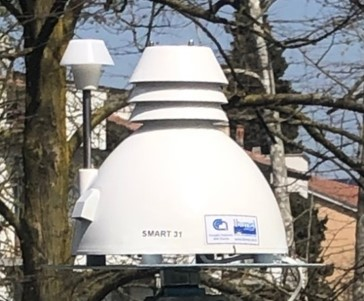
\includegraphics[width=0.50\textwidth,height=\textheight,keepaspectratio]{img/airqino_stazione}
\caption{Una centralina AirQino\\Fonte: \url{https://airqino.it}}
\label{fig:airqino_stazione}
\end{figure}

La rete di sensori AirQino consente rilevare le principali sostanze inquinanti riscontrabili nell’aria (\ce{NO2}, \ce{O3}, \ce{CO}, \ce{PM_{2.5}}, \ce{PM_{10}}) ma anche ulteriori parametri ambientali, come la temperatura, l'umidità relativa dell’aria e il principale gas climalterante, la \ce{CO2} (tabella \ref{fig:sensori-airqino}).
Inoltre la centralina è estendibile, e permette di aggiungere ulteriori sensori ausiliari in base alle preferenze.

\begin{table}[H]
    \footnotesize
    \centering
    \def\arraystretch{0.9}
    \begin{tabular}{|l|l|l|l|l|l|}
    \hline
        \textbf{Sensori} & \textbf{Tipologia} & \textbf{Unità} & \textbf{Range} & \textbf{Prec.} \\ \hline
        \ce{NO2} & Sensori di gas MOS & $\mathrm{\si{\micro}g/m^3}$ & 0-5000 & 15\% \\ \hline
        \ce{O3} & Semiconduttore & $\mathrm{\si{\micro}g/m^3}$ & 0-1000 & 15\% \\ \hline
        CO & Sensori di gas MOS & $\mathrm{\si{\micro}g/m^3}$ & 0-30 & 15\% \\ \hline
        VOC totali & Sensori di gas MOS & $\mathrm{\si{\micro}g/m^3}$ & 0-1000 & 15\% \\ \hline
        \ce{CO2} & NDIR & ppm o $\mathrm{\si{\micro}g/m^3}$ & 0-2000 & 10\% \\ \hline
        \ce{PM_{2.5}} & Contatore di particelle ottico & $\mathrm{\si{\micro}g/m^3}$ & 0-1000 & 10\% \\ \hline
        \ce{PM10} & Contatore di particelle ottico & $\mathrm{\si{\micro}g/m^3}$ & 0-1000 & 10\% \\ \hline
        Umidità relativa & Stato solido & \% & 0-100 & 5\% \\ \hline
        Temp. dell’aria & Stato solido & °C & -40 - 80 & 5\% \\ \hline
        Temp. interna & Stato solido & °C & -40 - 80 & 5\% \\ \hline
    \end{tabular}
    \caption{Tipologie di sensori in dotazione con le centraline AirQino (configurazione base, estendibile). Fonte: \url{https://airqino.it}}
    \label{fig:sensori-airqino}
\end{table}

Lato frontend, la pagina si apre su mappa interattiva che visualizza tutte le reti di centraline. Selezionata una stazione di interesse, vengono mostrati dettagli e foto della stazione stessa (figura \ref{fig:airqino}). Per ciascun sensore della centralina selezionata è possibile visualizzare grafici di andamento medio settimanali, insieme al dato istantaneo relativo all'ultima misurazione.

\begin{figure}[H]
\centering
\captionsetup{justification=centering}
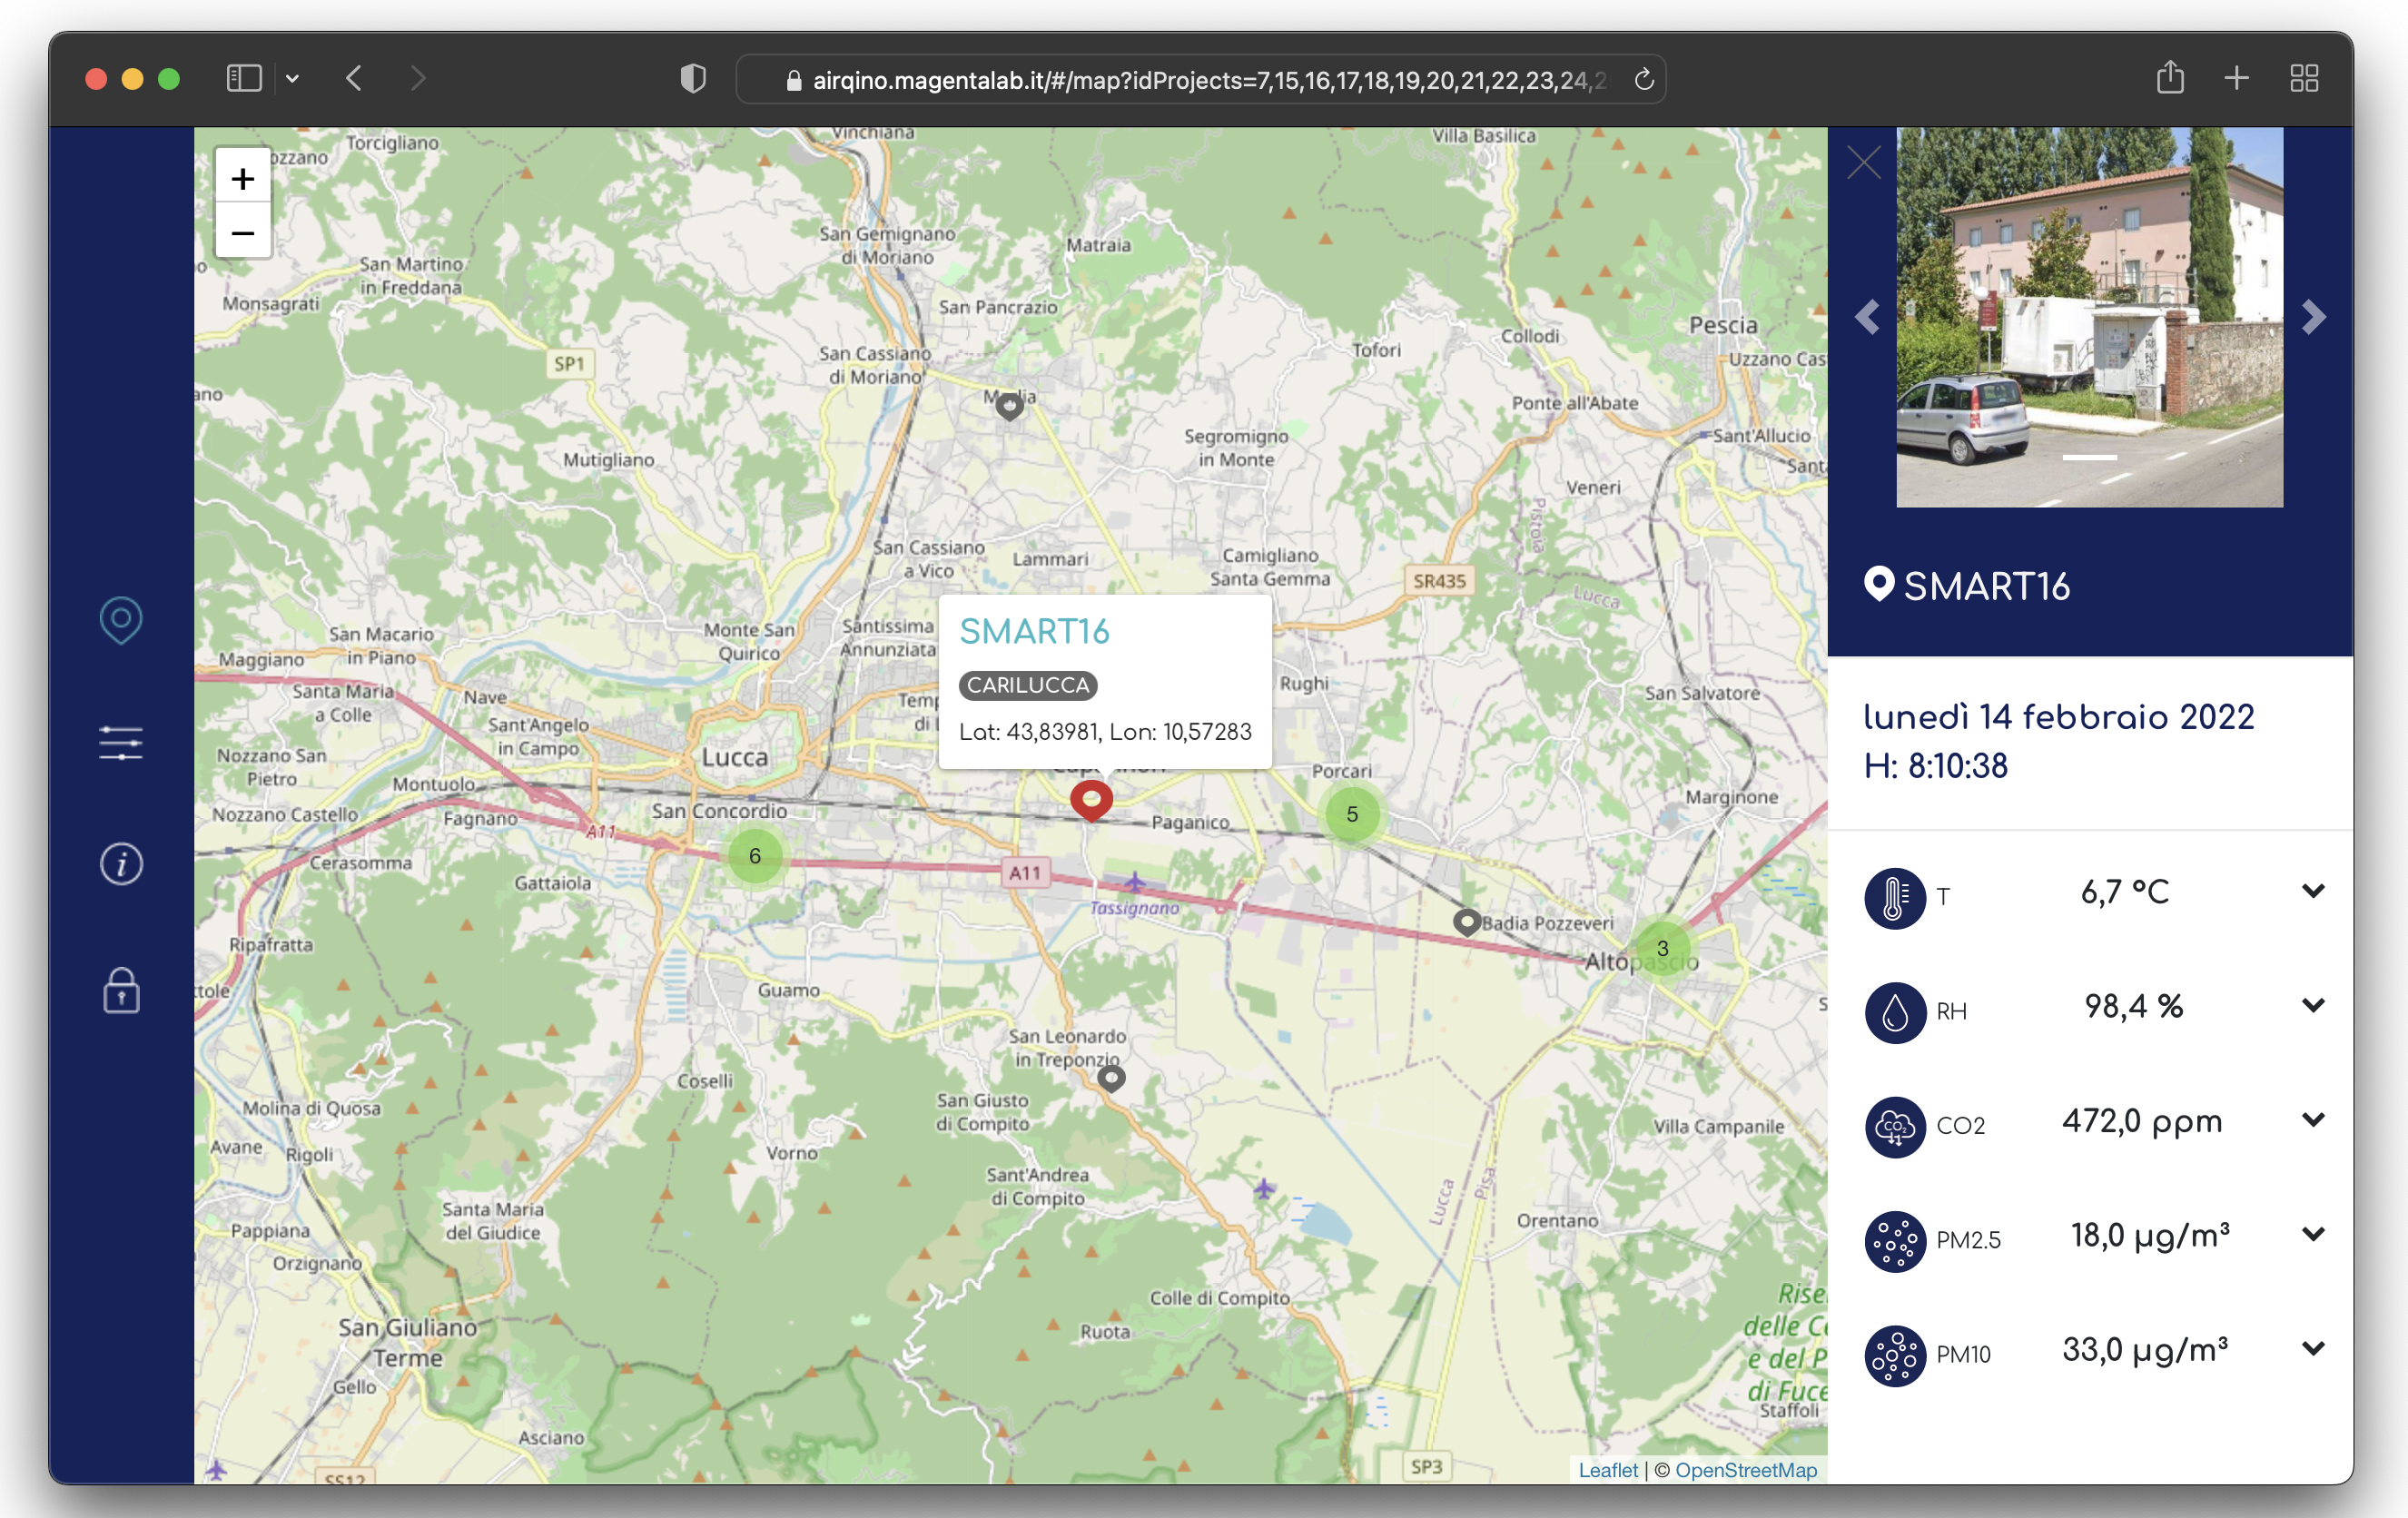
\includegraphics[width=0.70\textwidth,height=\textheight,keepaspectratio]{img/airqino_web}
\caption{La piattaforma web di AirQino\\Fonte: \url{https://airqino.magentalab.it}}
\label{fig:airqino}
\end{figure}

\subsection{Architettura e tecnologie}\label{ssec:airqino-architettura}
Il sistema è composto dai seguenti elementi principali:

\begin{itemize}
  \item \textbf{Gateway}: server che espone servizi compatibili con le centraline, e normalizza i dati trasmessi verso il server di raccolta. Questa applicazione, realizzata con Java e framework \textbf{Spring} \cite{spring}, fornisce un endpoint con lo stesso indirizzo a cui le centraline comunicano, in modo da garantire continuità di servizio. Il gateway ha anche il compito di segnalare eventuali interruzioni di funzionamento, secondo regole ben definite. Il gateway produce anche un output su protocollo \textit{MQTT2}, utilizzando un broker open source per pubblicare i dati verso il backend;
  \item \textbf{Backend}: applicazione server che si interfaccia con il broker \textit{MQTT} e scrive sul database i dati, esponendo inoltre servizi web di tipo REST utilizzati dal frontend web. Il backend è realizzato con Java e framework \textbf{Spring} \cite{spring} e utilizza \textbf{Timescale} \cite{timescale}, un database relazionale open source per la gestione efficienti di dati temporali;
  \item \textbf{Frontend}: applicazione web che permette la visualizzazione di mappa e grafici dei dati raccolti dalle centraline, utilizzando i servizi esposti dal backend. L'interfaccia è basata su tecnologia \textbf{Angular} \cite{angular}. Il frontend ha anche una sezione \textit{admin}, protetta da autenticazione, che permette la gestione del sistema. Le funzionalità di gestione previste sono:
    \begin{itemize}
      \item Gestione anagrafica centraline (nome, posizione, progetti a cui afferisce);
      \item Configurazione dei parametri di funzionamento tra cui i parametri di calibrazione, per la trasformazione da dati grezzi a valori leggibili dall’utente, e le soglie rilevamento allarmi;
      \item Gestione utenti;
      \item Scaricamento dati raw oppure convertiti.
    \end{itemize}
\end{itemize}

\subsection{Hardware dei sensori}\label{ssec:hardware}
% todo schematics
Per quanto riguarda la caratteristiche dei sensori, i sensori di tipo MOS sono costituiti da un film (credo allumina? Per  fabbricare  gli  strati  sensibili  del  film,  si  prepara  una  pasta  viscosa:  al  materiale funzionale,  sotto  forma  di  polvere,  viene  aggiunta  una  miscela  di  agenti  reologici  in  solventi  volatili) depositato su una piastra di elementi riscaldanti la cui temperatura operativa è generalmente compresa tra 300 e 500°C. Di solito il  materiale funzionale del film più  adatto per  la  rilevazione di  biossido  di  azoto è l’ossido  di  ferro  e lantanio (LaFeO3) che oltre ad avere una buona sensibilità agli ossidi di azoto ha una  bassa  sensibilità  al  monossido  di  carbonio. Per la rilevazione dell’ozono viene invece utilizzato  triossido di tungsteno (WO3). Questo tipo  di  materiale  funzionale risulta  molto  sensibile  ai  gas  ossidanti  come  O3 e  NO2. Qualsiasi sia il materiale funzionale, il principio di funzionamento per tutti i MOS nella rilevazione di gas è quello di interagire con il gas presente all’interno dell’atmosfera tramite reazioni di ossidoriduzione, portando a un cambiamento di conduttività, che viene rilevato da un circuito apposito. Le variazioni della conduttività dei sensori è fortemente influenzata dalle variazioni di umidità e temperatura, come rilevato dalla letteratura sull'argomento [ref]. Nel caso dei sensori Mics che noi utilizziamo, il produttore non rilascia informazioni sull'influenza nella lettura dovuto alla temperatura/umidità  ma che queste influiscono può essere ipotizzato come può essere ipotizzato che ci sia una influenza introdotta dalla temperatura nel circuito ADC del microcontrollore.

Questo segnale viene passato al convertitore analogico digitale del controllore che lo trasforma in counts (10 bit da 0 a 2 alla 10).

ossidoriduzione → piastra che si scalda a seconda dell'inquinante genera corrente

il segnale viene passato attraverso un convertitore analogico digitale e l’uscita è a 10 bit (questa unità la chiamo counts)

\subsection{Progetti correlati}\label{ssec:correlati}
Di seguito sono elencati alcuni progetti che fanno uso delle centraline AirQino:

\begin{itemize}
  \item \textbf{Prato Urban Jungle} \cite{urbanjungle} mira a promuovere la progettazione urbana creativa e visionaria per ri-naturalizzare i quartieri di Prato in modo sostenibile e socialmente inclusivo;
  \item \textbf{SMART Treedom} \cite{smartreedom} è il frutto dalla collaborazione tra Treedom e l’Istituto di Biometeorologia del Consiglio Nazionale delle Ricerche. La finalità del progetto è stata quella di prototipare un sistema integrato che possa essere modulato con diversi sensori in base al tipo di grandezza fisica che si vuole misurare e una tecnologia laser per la misura delle polveri sottili;
  \item \textbf{Trafair} \cite{trafair} è un progetto europeo biennale co-finanziato dal programma europeo Connecting Europe Facility (CEF) nel settore delle telecomunicazioni con lo scopo di sviluppare un servizio di previsione della qualità dell’aria urbana basata su previsioni meteo e flussi di traffico in sei città europee di dimensioni diverse: Zaragoza, Firenze, Modena, Livorno, Santiago de Compostela e Pisa.
  \item \textbf{Smart Garda Lake} \cite{garda} nasce nel 2017 con lo scopo di creare una rete di monitoraggio ambientale per rilevamenti in campo meteorologico, inquinamento acustico, stato delle acque superficiali e qualità dell’aria all’insegna degli obiettivi di sostenibilità dell’Agenda 2030 dell’ONU;
  \item \textbf{Brenner LEC} \cite{lec} si colloca nel contesto di un’area sensibile come le Alpi e si pone l’obiettivo di creare un “corridoio a emissioni ridotte” (LEC – Lower Emission Corridor) lungo l’asse autostradale del Brennero al fine di ottenere un chiaro beneficio ambientale nei settori della tutela dell’aria e della protezione del clima, nonché una riduzione dell’inquinamento acustico.
\end{itemize}

\subsection{Progetti simili}\label{ssec:competitor}
Ci sono anche altre piattaforme simili ad AirQino:

\begin{itemize}
	\item \textbf{Airly} \cite{airly} è una piattaforma che consente di condividere informazioni ambientali in tempo reale, grazie alla quale è possibile monitorare la qualità dell'aria e i livelli di inquinamento;
	\item \textbf{Aqicn} \cite{aqicn} è un progetto open source lanciato nel 2010 che consente di monitorare l'inquinamento atmosferico in tempo reale;
	\item \textbf{IQAir} \cite{iqair} è una società svizzera che produce e vende purificatori d'aria per uso residenziale e commerciale. La loro applicazione fornisce un rapporto in tempo reale sulla qualità dell'aria e previsione dell'inquinamento atmosferico;
	\item \textbf{Decentlab} \cite{decentlab} è un'azienda svizzera che fornisce dispositivi e servizi di sensori wireless per soluzioni di monitoraggio distribuite ed economiche;
	\item \textbf{PlanetWatch} \cite{planetwatch} è una piattaforma decentralizzata che consente di monitorare e proteggere il pianeta attraverso la condivisione di informazioni. Gli utenti possono condividere informazioni sull'ambiente, la sostenibilità e la responsabilità sociale;
	\item \textbf{HackAIR} \cite{hackair} è una piattaforma open source che consente ai cittadini di monitorare la qualità dell'aria nei propri quartieri. Gli utenti possono interagire con la piattaforma per segnalare la qualità dell'aria nel proprio quartiere, visualizzare i dati relativi alla qualità dell'aria e condividere informazioni e dati con altri utenti.
\end{itemize}


\mainmatter
\chapter{Sviluppi tecnologici}\label{ch:sviluppi}
Questo capitolo riguarda i miglioramenti realizzati dal punto di vista tecnologico che sono andati direttamente ad impattare la piattaforma AirQino, migliorandone in un caso l'affidabilità dei dati e nell'altro i tempi di risposta del database per query particolarmente onerose.

% Replica del database di produzione
\section{Replica del database di produzione}\label{sec:replica}

Spesso fare analisi mediamente complesse sui dati contenuti in un database può comportare rallentamenti nei tempi di risposta. Se questi carichi risultano frequenti, il sistema può arrivare a bloccarsi e interrompere il servizio.

Una soluzione per risolvere questo problema è la creazione di una (o più) repliche del database primario. Nella replica, i dati e gli oggetti del database vengono copiati e distribuiti su un altro spazio fisico. Le operazioni onerose a questo punto possono essere fatte direttamente sulla replica che agisce come nodo secondario: in questo modo, il carico viene distribuito e non si intaccano le performance del database principale.

Il concetto di \textit{replica} è diverso dal \textit{mirroring}, in cui vengono create una o più copie di un database su diverse istanze del server, e funzionano come copie di riserva (e si attivano soltanto nel caso di guasto del nodo principale).

Un sistema di replica correttamente implementato può offrire diversi vantaggi, tra cui riduzione del carico (perchè i dati replicati possono essere distribuiti su più server), efficienza (i server offrono prestazioni migliori perchè meno gravati da query pesanti) e ridondanza (i dati sono raggiungibili da più indirizzi).

Di contro, questa tecnica comporta la necessità di mantenimento dei nodi secondari, spesso collocati su server diversi (con i costi a questi associati). Inoltre, repliche errate o non implementate in maniera corretta possono causare la mancata sincronizzazione tra i nodi, portando ad una perdita o incoerenza dei dati.

\subsection{Motivazioni}\label{ssec:replica-motivazioni}
L'affidabilità dei dati rappresenta uno dei punti critici per un sistema di ingestione di grosse quantità di dati. Questo è vero anche caso di AirQino, dove infatti il database di produzione conta oltre 100 milioni di misurazioni rilevate, in continuo aumento con una media di 300 inserimenti al minuto.

La replica offrire vantaggi in questo senso, principalmente legati alle prestazioni, disponibilità e sicurezza dei dati:
\begin{enumerate}
  \item \textbf{Maggiore affidabilità}: tramite la replica del database viene garantita la disponibilità dei dati anche nel caso in cui una delle macchine presenti un guasto hardware. In questo caso, il sistema di gestione del database distribuito deve essere in grado di indirizzare gli utenti interessati ad uno degli altri nodi disponibili;
  \item \textbf{Miglioramento delle prestazioni}: essendo i dati distribuiti su diverse istanze, accessi multipli non saturano i server. Questo aspetto risulta particolarmente importante per applicazioni che possono avere una grande quantità di richieste simultanee;
  \item \textbf{Maggiore sicurezza dei dati}: Mentre in un sistema tradizionale i backup di un database (se effttuati) sono archiviati sullo stesso disco, con la replica del database vengono scritti su più server, aumentandone di fatto l'affidabilità e la ridondanza.
\end{enumerate}

Esistono diverse tecniche di replicazione del database, che dipendono sia dalla tecnologia utilizzata (MySQL, Postgres) che dalla natura del database stesso (relazionale o non relazionale). Il database di AirQino fa uso di Timescale\footnote{Timescale: Time-series data simplified - \url{https://www.timescale.com}}, basato su Postgres; una caratteristica di Postgres è la possibilità di replicazione con la tecnologia di \textbf{Streaming Replication}, descritta di seguito.

\subsection{Streaming replication}\label{ssec:streaming-replication}
La streaming replication di PostgreSQL è una funzionalità che consente di replicare i dati in tempo reale da una istanza di PostgreSQL a un'altra. Questo significa che, se si modificano i dati in una delle istanze, questi saranno immediatamente replicati anche nell'altra istanza. Questa istanza database di replica di lettura ("standby" in termini PostgreSQL) è una replica fisica creata in modo asincrono dell'istanza del database primario.

PostgreSQL fa utilizza un ruolo di "replica" (\textit{replication role}) per eseguire la replica in streaming (il ruolo presenta dei privilegi ma non può essere utilizzato per modificare i dati, la replica infatti è di sola lettura).

La replica si basa sulle transazioni WAL (Write Ahead Log) e utilizza il protocollo TCP per garantire una connessione sicura tra i server e inviare in modo asincrono le modifiche al database via via che vengono effettuate.

È possibile promuovere una replica di lettura PostgreSQL a una nuova istanza database di origine. Una volta promossa, la replica smette di ricevere comunicazioni WAL e non è più un'istanza di sola lettura.

PostgreSQL salva le informazioni aggiornate del server primario in registro delle transazioni, noto come registro \textit{write-ahead}, utile in preparazione per il ripristino da crash o il rollback. La replica in streaming funziona proprio trasferendo e applicando il WAL al server di replica in tempo reale.

\begin{figure}[H]
\centering
\captionsetup{justification=centering}
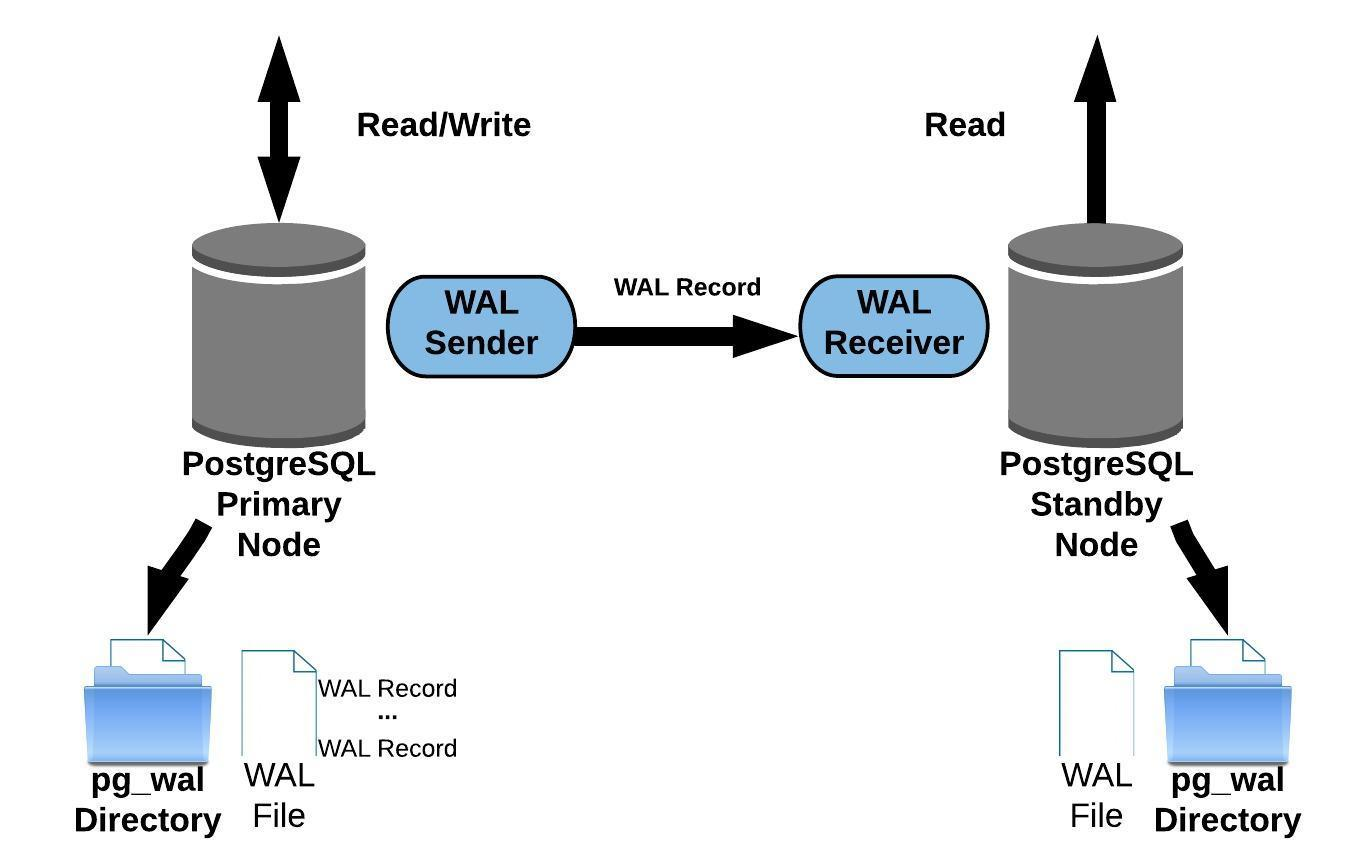
\includegraphics[width=0.75\textwidth,height=\textheight,keepaspectratio]{img/streaming_replication.jpg}
\caption{Streaming Replication di PostgreSQL\\Fonte: \url{https://severalnines.com}}
\label{fig:streaming-replication}
\end{figure}

La replica in streaming può essere costruita in una configurazione 1:N, in cui è configurabile un solo server primario, ma è possibile configurare più server di replica (configurazione \textit{multi-standby}). È anche possibile creare una configurazione a cascata in cui un server di replica si connette ad un altro server di replica.

Per la replica in streaming, è possibile scegliere se effettare una replica sincrona o asincrona. La differenza tra replica sincrona e replica asincrona sta nell'attesa o meno della risposta dal server di replica prima di completare l'elaborazione sul server primario:
\begin{itemize}
  \item \textbf{Replica sincrona}: il server primario attende una risposta dal server di replica prima di completare un processo. In questo caso il tempo di risposta complessivo include anche il tempo di spedizione del registro;
  \item \textbf{Replica asincrona} (impostazione predefinita): il server primario completa un processo senza attendere una risposta dal server di standby. Pertanto, il tempo di risposta complessivo è più o meno lo stesso di quando non viene utilizzata la replica in streaming; in questa modalità il risultato aggiornato sul server primario potrebbe non essere immediatamente disponibile sul server di replica. \cite{streaming_replication}
\end{itemize}

Esistono di contro diverse limitazioni per le repliche con PostgreSQL:
\begin{itemize}
  \item Ogni replica di lettura PostgreSQL è di sola lettura. Non è possibile creare una replica di lettura che sia scrivibile;
  \item Non è possibile creare una replica di lettura da un'altra replica di lettura a cascata;
  \item Gli utenti e i ruoli di accesso vengono rispecchiati dall'istanza primaria, il che significa che non è possibile utilizzare credenziali diverse o aggiungere utenti aggiuntivi soltanto alla replica;
  \item Non è possibile creare tabelle e viste nell'istanza di replica; in pratica dalla replica si possono solo eseguire query di tipo \textit{SELECT}.
\end{itemize}

\subsubsection{Preparazione del database primario}

\begin{enumerate}
  \item Per avviare la procedura si crea sul database un utente PostgreSQL con un ruolo adatto ad avviare la streaming replication:
  \vspace{1mm}
   \begin{lstlisting}[language=sql]
SET password_encryption = 'scram-sha-256'; 
CREATE ROLE repuser WITH REPLICATION PASSWORD 'SOME_SECURE_PASSWORD' LOGIN;\end{lstlisting}
  \item Aggiungere i seguenti parametri al file \url{/var/lib/postgresql/data/postgresql.conf}:
  \vspace{1mm}
  \begin{lstlisting}[]
listen_addresses= '*'
wal_level = replica
max_wal_senders = 2
max_replication_slots = 2
synchronous_commit = off
\end{lstlisting}

  \item Aggiungere i seguenti parametri al file di configurazione \url{/var/lib/postgresql/data/pg_hba.conf} per configurare l'autenticazione basata su host in modo da accettare connessioni dalla replica\footnote{Dalla documentazione Streaming Replication: \url{https://www.postgresql.org/docs/current/warm-standby.html\#STREAMING-REPLICATION}}:
  \vspace{1mm}
\begin{lstlisting}[]
host     replication     repuser   <REPLICA_IP>/32       scram-sha-256
\end{lstlisting}
dove \textit{repuser} è l'utente creato al passo 1 e \textit{REPLICA\_IP} è l'IP della macchina in cui si trova la replica;
  \item Riavviare il database per applicare i cambiamenti;
  \item Infine creare uno slot di replicazione sul database:
  \vspace{1mm}
  \begin{lstlisting}[language=sql]
SELECT * FROM pg_create_physical_replication_slot('replica_1_slot');
\end{lstlisting}
\end{enumerate}

\subsubsection{Configurazione della replica}
Di seguito sono elencati i passi da seguire per configurare la replica:

\begin{enumerate}
  \item Stoppare l'istanza Postgres:
  \vspace{1mm}
\begin{lstlisting}[]
pg_ctl -D $PGDATA -m fast -w stop
\end{lstlisting}
  \item Cancellare i contenuti della cartella \textit{PGDATA}:
  \vspace{1mm}
\begin{lstlisting}[]
rm -rf $PGDATA/*
\end{lstlisting}
  \item Avviare il backup del database primario:
  \vspace{1mm}
\begin{lstlisting}[]
pg_basebackup -h <PRIMARY_HOST> -p <PRIMARY_PORT> -D $PGDATA -U repuser -vP -R -W
\end{lstlisting}
Dove \textit{PRIMARY\_HOST} è l'IP della macchina in cui si trova il database primario, \textit{PRIMARY\_PORT} è la porta del database primario e \textit{repuser} è l'utente di replicazione creato al passo 1.

Da notare che verrà chiesta in maniera interattiva la password di replicazione impostata in precedenza (\textit{SOME\_SECURE\_PASSWORD});
  \item Infine avviare l'istanza Postgres:
  \vspace{1mm}
\begin{lstlisting}[]
pg_ctl -D $PGDATA -w start
\end{lstlisting}
A questo punto la replica dovrebbe essere funzionante e sincronizzata 1:1 in tempo reale con il database primario.
\end{enumerate}

\subsubsection{Automazione con Docker}
L'intero setup (sia database primario che la replica) può essere automatizzato con Docker e docker-compose, in modo da far partire la sincronizzazione all'avvio del container.
Poichè i passi per creare la replica richiedono di stoppare l'istanza Postgres, non si può eseguire all'interno del container Docker già avviato perchè si stopperebbe tutto il container.
Per questo è necessario dare i comandi per la replica da uno script di \textit{entrypoint} che viene eseguito prima di avviare il container:
\begin{enumerate}
  \item Creare un Dockerfile da immagine Timescale (\url{timescaledb:latest}), con l'aggiunta di uno script \textit{entrypoint}, così strutturato:
  \vspace{1mm}
  \begin{lstlisting}[]
FROM timescale/timescaledb:latest-pg13
ADD replica.sh /docker-entrypoint-initdb.d/
\end{lstlisting}
  \item Creare il file \url{replica.sh} che verrà eseguito tutte le volte che si avvia il database:
  \vspace{1mm}
  \begin{lstlisting}[]
echo "Stopping Postgres instance..." 
pg_ctl -D ${PGDATA} -m fast -w stop

echo "Clearing PGDATA folder..." 
rm -rf ${PGDATA}

echo "Creating base backup..." 
PGPASSWORD=${REPLICATION_PASSWORD} pg_basebackup -h ${REPLICATION_HOST} -p ${REPLICATION_PORT} -D ${PGDATA} -U ${REPLICATION_USER} -vP -R -w

echo "Restarting Postgres instance..." 
pg_ctl -D ${PGDATA} -w start
\end{lstlisting}
Da notare che la flag -W di \textit{pg\_basebackup} chiede la password in maniera interattiva, che non funziona per script automatizzati. Come alternativa si può usare la flag -w (minuscola) e passare la password come variabile di ambiente chiamata \textit{PGPASSWORD};
\item Creare il file docker-compose.yml:
\vspace{1mm}
  \begin{lstlisting}[]
services:
  replica:
    build:
        context: .
        dockerfile: Dockerfile
    environment:
        # Cartella PDATA custom
        PGDATA: /var/lib/postgresql/data/pgdata

        # Parametri di replicazione
        REPLICA_USER: repuser # Utente di replicazione impostato al punto 1
        REPLICATION_HOST: x.x.x.x # IP del db primario
        REPLICATION_PORT: x # Porta del db primario
        REPLICATION_PASSWORD: SOME_SECURE_PASSWORD # Password di replicazione impostata al punto 1
    ports:
        - 45432:5432
    volumes:
        - /var/replica-pg13-timescale/:/var/lib/postgresql/data
\end{lstlisting}

  \item Avviare il container con \url{docker-compose} \url{up}.
\end{enumerate}

In questo modo la replica verrà sincronizzata con il database primario automaticamente all'avvio del container Docker.
Allo stesso modo è possibile automatizzare con Docker anche il setup su database primario.

% Ottimizzazione di query temporali
\section{Ottimizzazione di query temporali}\label{sec:cont-aggr}
% todo metti percentuale? es. tempo sceso di X%
Ci sono molti vantaggi nell'aggregazione di dati:
\begin{itemize}
  \item \textbf{Flessibilità}: aggregare dati in tempo reale in base a qualsiasi criterio desiderato;
  \item \textbf{Risparmio di tempo}: non è necessario eseguire query aggiuntive per ottenere informazioni aggregate in tempo reale;
  \item \textbf{Risparmio di spazio} i dati aggregati in tempo reale occupano meno spazio rispetto ai dati non aggregati.
\end{itemize}

I dati delle serie temporali però tendono a crescere molto rapidamente, e grandi volumi di dati possono rallentare quando si eseguono query con lo scopo di aggregare i dati (ad esempio per generare report o riepiloghi sull'andamento).

Per garantire efficienza e scalabiità con questa tipologia di dati, si rende quindi necessario garantire che le query su dati temporali abbiano un tempo di risposta costante, indipendentemente dalla quantità di dati e senza gravare sul database.

\subsection{Motivazioni}\label{ssec:cont-aggr-motivazioni}
La piattaforma AirQino (vedi \ref{sec:airqino}) raccoglie dati emessi ogni minuto da decine di centraline in diverse località. Per memorizzare questi dati viene utilizzato un database Postgres con estensione Timescale, che offre delle funzionalità specifiche proprio per dati di tipo temporale.

Una delle funzionalità di AirQino consente di mostrare un grafico dell'andamento (su base media oraria) dell'ultima settimana per diverse grandezze (temperatura, umidità, \ce{CO2}, \ce{NO2}, \ce{PM_{2.5}}, \ce{PM_10} ecc..), come mostrato in figura \ref{fig:airqino-temp}.

\begin{figure}[H]
\centering
\captionsetup{justification=centering}
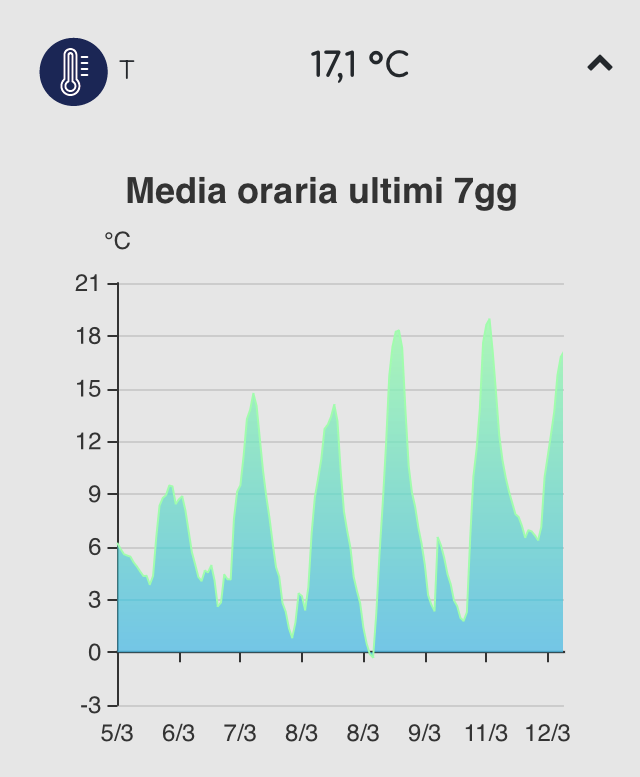
\includegraphics[width=0.45\textwidth,height=\textheight,keepaspectratio]{img/airqino_temp}
\caption{Grafico dell'andamento della temperatura nell'ultima settimana per una centralina AirQino.\\Fonte: \url{https://airqino.magentalab.it}}
\label{fig:airqino-temp}
\end{figure}

Attualmente sono previsti i seguenti casi d’uso dei dati a media oraria:
\begin{itemize}
  \item Visualizzazione sulla home page dell’applicazione web degli ultimi 7 giorni;
  \item Esportazione dataset periodici da mettere a disposizione degli utenti esterni (ad esempio pubbliche amministrazioni che hanno installato le centraline);
  \item Esportazione dataset on demand da parte di utenti esterni, con indicazione di inizio/fine del periodo desiderato.
\end{itemize}
In tutti questi casi il requisito è di ottenere medie orarie del dato calibrato.

Per calcolare la media oraria nell'ultima settimana, ad ogni richiesta sul database viene eseguito una query SQL di questo tipo (ridotta per semplicità):

\vspace{1mm}
\begin{lstlisting}[language=sql]
SELECT time_bucket('1 hour', sd.data_acquired) as bucket, avg(sd.float_value)
FROM station_data sd
WHERE sd.data_acquired > NOW() - INTERVAL '7 days'
AND sd.sensor_id = 29510691 /* id centralina */
ORDER BY bucket DESC;
\end{lstlisting}

La query fa uso della funzione \textit{time\_bucket} di Timescale, che consente di partizionare la tabella con i dati dei sensori minuto per minuto direttamente in fasce orarie. L'utilizzo combinato con la funzione \textit{avg()} va poi a prendere la media del valore su tutta l'ora.

Questo però significa che se si desidera eseguire questa query più di una volta, il database deve eseguire la scansione dell'intera tabella e ricalcolare la media ogni volta. Nella maggior parte dei casi, tuttavia, i dati nella tabella non sono cambiati in modo significativo, quindi non è necessario eseguire la scansione dell'intero set di dati.

La figura \ref{fig:query-prima} mostra i tempi di risposta a questa query per tutte le centraline AirQino prima di aver applicato l'ottimizzazione.

\begin{figure}[H]
\centering
\captionsetup{justification=centering}
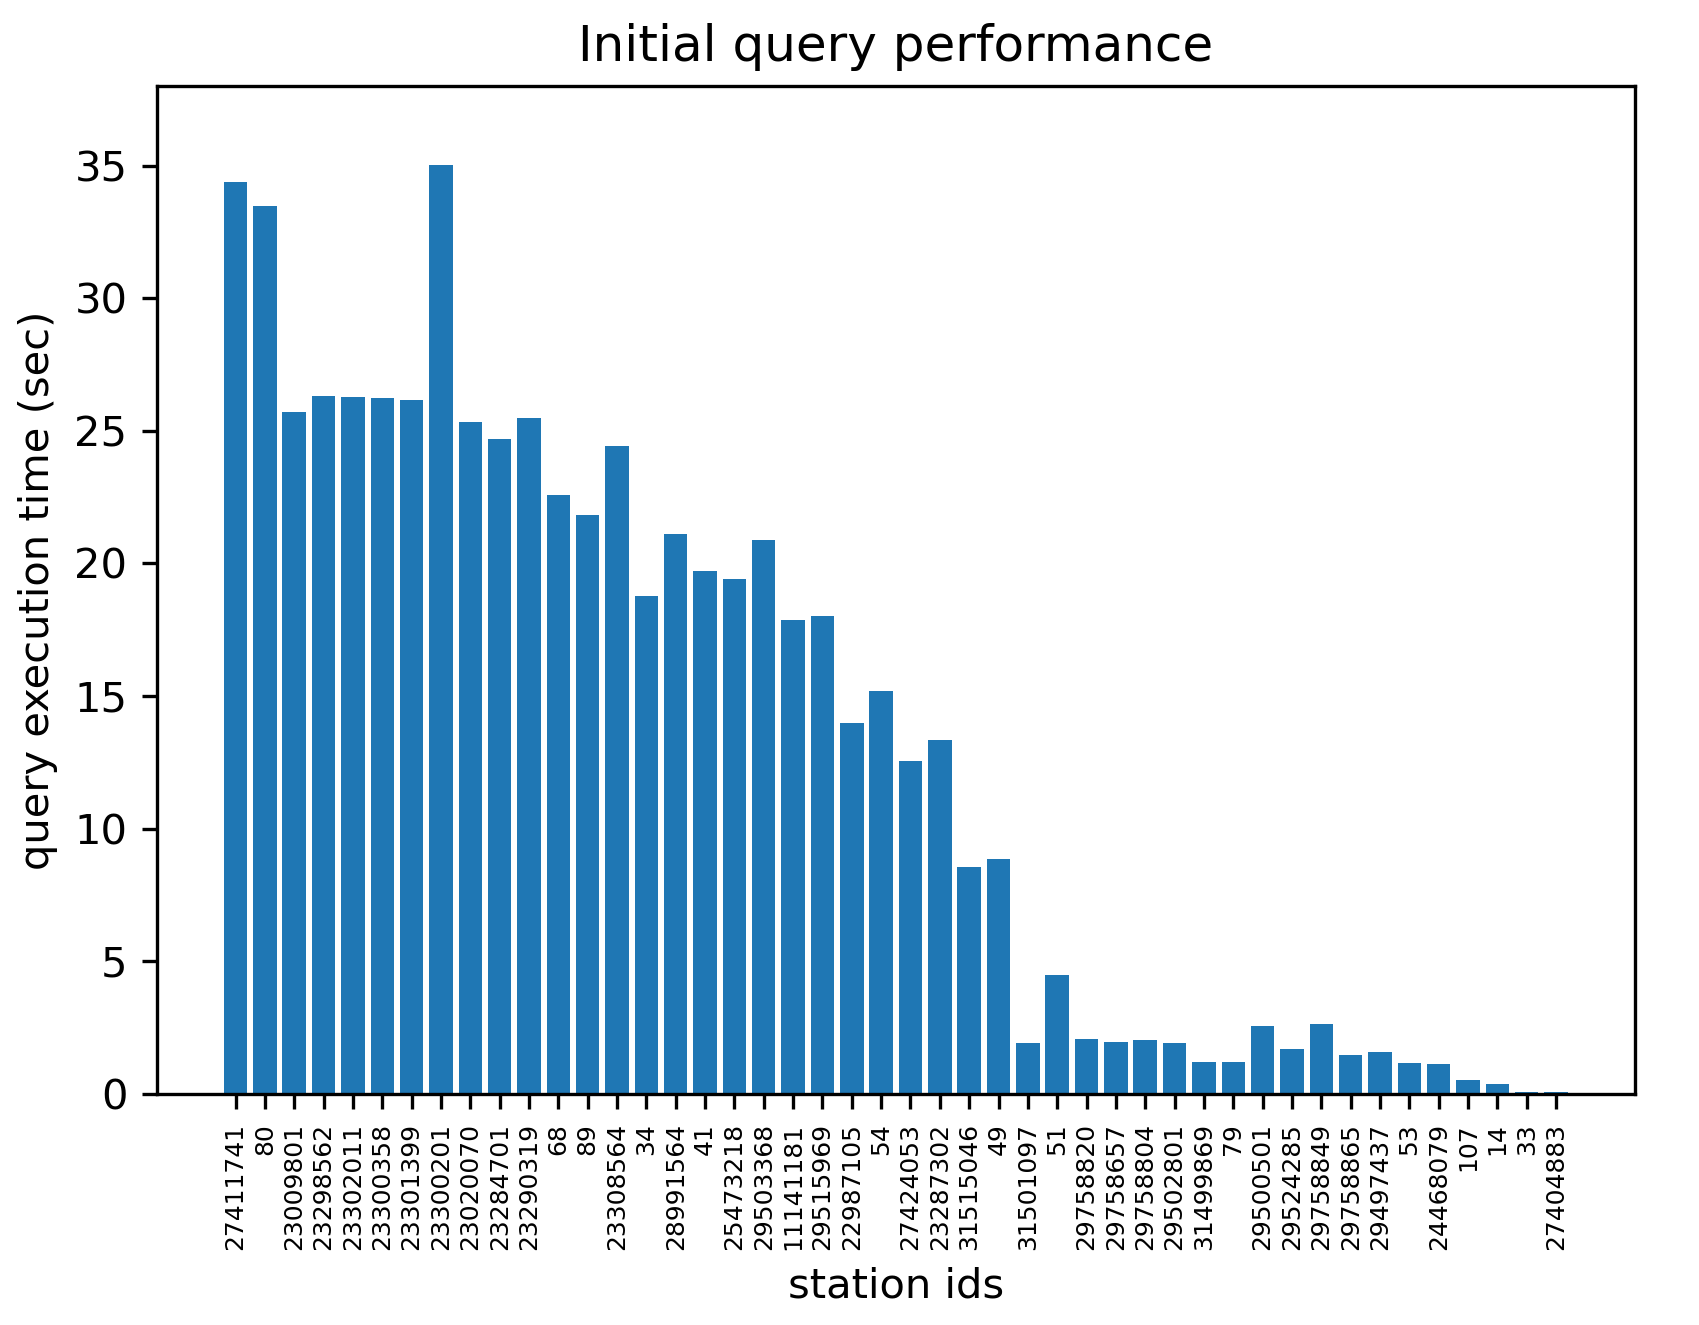
\includegraphics[width=0.85\textwidth,height=\textheight,keepaspectratio]{img/query_prima}
\caption{Tempi di risposta per query temporali sulle centraline AirQino prima dell'ottimizzazione (media su 10 iterazioni)}
\label{fig:query-prima}
\end{figure}

Come si può vedere, per le centraline più attive la query per recuperare la media oraria impiega fino a 35 secondi, un tempo molto elevato.

Per rendere più veloce l'aggregazione dei dati, Timescale mette a disposizione una funzionalità chiamata \textbf{continuous aggregates} (\textit{aggregati continui}), spiegata di seguito.

\subsection{Continuous aggregates}\label{ssec:cont-aggr}
I continuous aggregate sono una funzionalità integrata in TimescaleDB che consente di aggregare i dati in tempo reale, senza la necessità di eseguire query aggiuntive. Funzionano in maniera simile alle viste materializzate di PostgreSQL, con la differenza che non necessitano di essere aggiornati manualmente ogni volta che un nuovo dato viene inserito nella tabella. Infatti, la riaggregazione viene eseguita automaticamente in background tramite una \textbf{refresh policy} definita dall'utente in fase di creazione della vista.

L’utilizzo dei countinuous aggregates offre diversi vantaggi:
\begin{itemize}
  \item Miglioramento delle \textbf{performance}, infatti non è più necessario scansionare tutte le volte la tabella con i dati raw ma è sufficiente leggere questi risultati precalcolati;
  \item Funzionalità avanzate, come la possibilità di salvare i dati raw solo per un periodo di tempo limitato, continuando però a mantenere i dati aggregati. Così facendo si hanno dei dati riassuntivi per eventi che sono molto indietro nel tempo, mentre per gli eventi più recenti si continua ad avere tutti i dati raccolti, portando and un grosso \textbf{risparmio di spazio occupato}.
\end{itemize}

Di contro, lo svantaggio di questa soluzione è che i dati non sono aggiornati ad ogni INSERT effettuata, ma solo ad un intervallo di tempo specificato dall’utente. Questo significa che in fase di lettura i dati più recenti non sono presenti nelle viste materializzate. Per limitare questo problema si potrebbe pensare di diminuire l’intervallo di tempo necessario per il refresh dei dati, ma questo porterebbe ad un aumento del carico computazionale. C'è quindi un compromesso tra la velocità di lettura e l’aggiornamento dei dati. \cite{tesi_polito_2}

Timescale inoltre introduce il concetto di \textit{hypertable}, normali tabelle SQL ma con partizionamento automatico su base temporale.

\subsection{Risultati ottenuti}\label{ssec:cont-aggr-risultati}
Di seguito sono riportati i passi eseguiti sul database di produzione AirQino per l'attivazione del meccanismo di continuous aggregates sulla tabella con i dati dei sensori (\textit{station\_data}):

\begin{enumerate}
  \item  Creare la \textit{hypertable} a partire dalla tabella originale, migrando tutti i dati:
\vspace{1mm}
\begin{lstlisting}[language=sql]
SELECT create_hypertable('station_data', 'data_acquired', migrate_data => true);
\end{lstlisting}
Dove \textit{data\_acquired} è la colonna temporale della tabella, in cui vengono salvati data e ora della misurazione.
Questa operazione potrebbe impiegare molto tempo, in base alla quantità di dati nella tabella. Sul database di produzione AirQino ha richiesto circa 36 minuti.
  \item Creare la vista materializzata per il calcolo delle medie orarie:
\vspace{1mm}
\begin{lstlisting}[language=sql]
CREATE MATERIALIZED VIEW station_data_hourly_avg
WITH (timescaledb.continuous) AS
SELECT time_bucket('1 hour', sd.data_acquired) AS bucket, 
    station_id,  
    sensor_id, 
    avg(sd.float_value) 
FROM station_data sd
GROUP by bucket, station_id, sensor_id;
\end{lstlisting}
Questa operazione sul database di produzione AirQino ha richiesto circa 5 minuti.
  \item Creare una refresh policy adeguata:
\vspace{1mm}
\begin{lstlisting}[language=sql]
SELECT add_continuous_aggregate_policy('station_data_hourly_avg',
     start_offset => INTERVAL '7 days',
     end_offset => INTERVAL '1 hour',
     schedule_interval => INTERVAL '1 hour');
\end{lstlisting}
Dove \textit{start\_offset} indica quanto indietro nel tempo vado a calcolare l'aggregato, \textit{end\_offset} indica fino a quando arrivo e schedule indica ogni quanto voglio refreshare la vista.
In questo caso voglio refreshare ogni ora i dati da una settimana fa fino a un'ora fa.
Per ragioni di performance conviene sempre escludere l'ultimo bucket (in questo caso l'ultima ora di dati arrivati).
\end{enumerate}

Una volta creata la vista, è possibile ricreare la SELECT originale per la media degli ultimi 7 giorni prendendo i dati da questa nuova tabella:
\vspace{1mm}
\begin{lstlisting}[language=sql]
SELECT sd.avg
FROM station_data_hourly_avg sd
WHERE bucket > NOW() - INTERVAL '7 days'
AND sd.sensor_id = 29510691 /* id centralina */
ORDER BY bucket DESC;
\end{lstlisting}

Questa nuova query è risultata molto più performante rispetto alla precedente, perchè le medie orarie sono di fatto già precalcolate. I risultati sulle centraline AirQino sono riportati di seguito in figura \ref{fig:query-dopo}.

\begin{figure}[H]
\centering
\captionsetup{justification=centering}
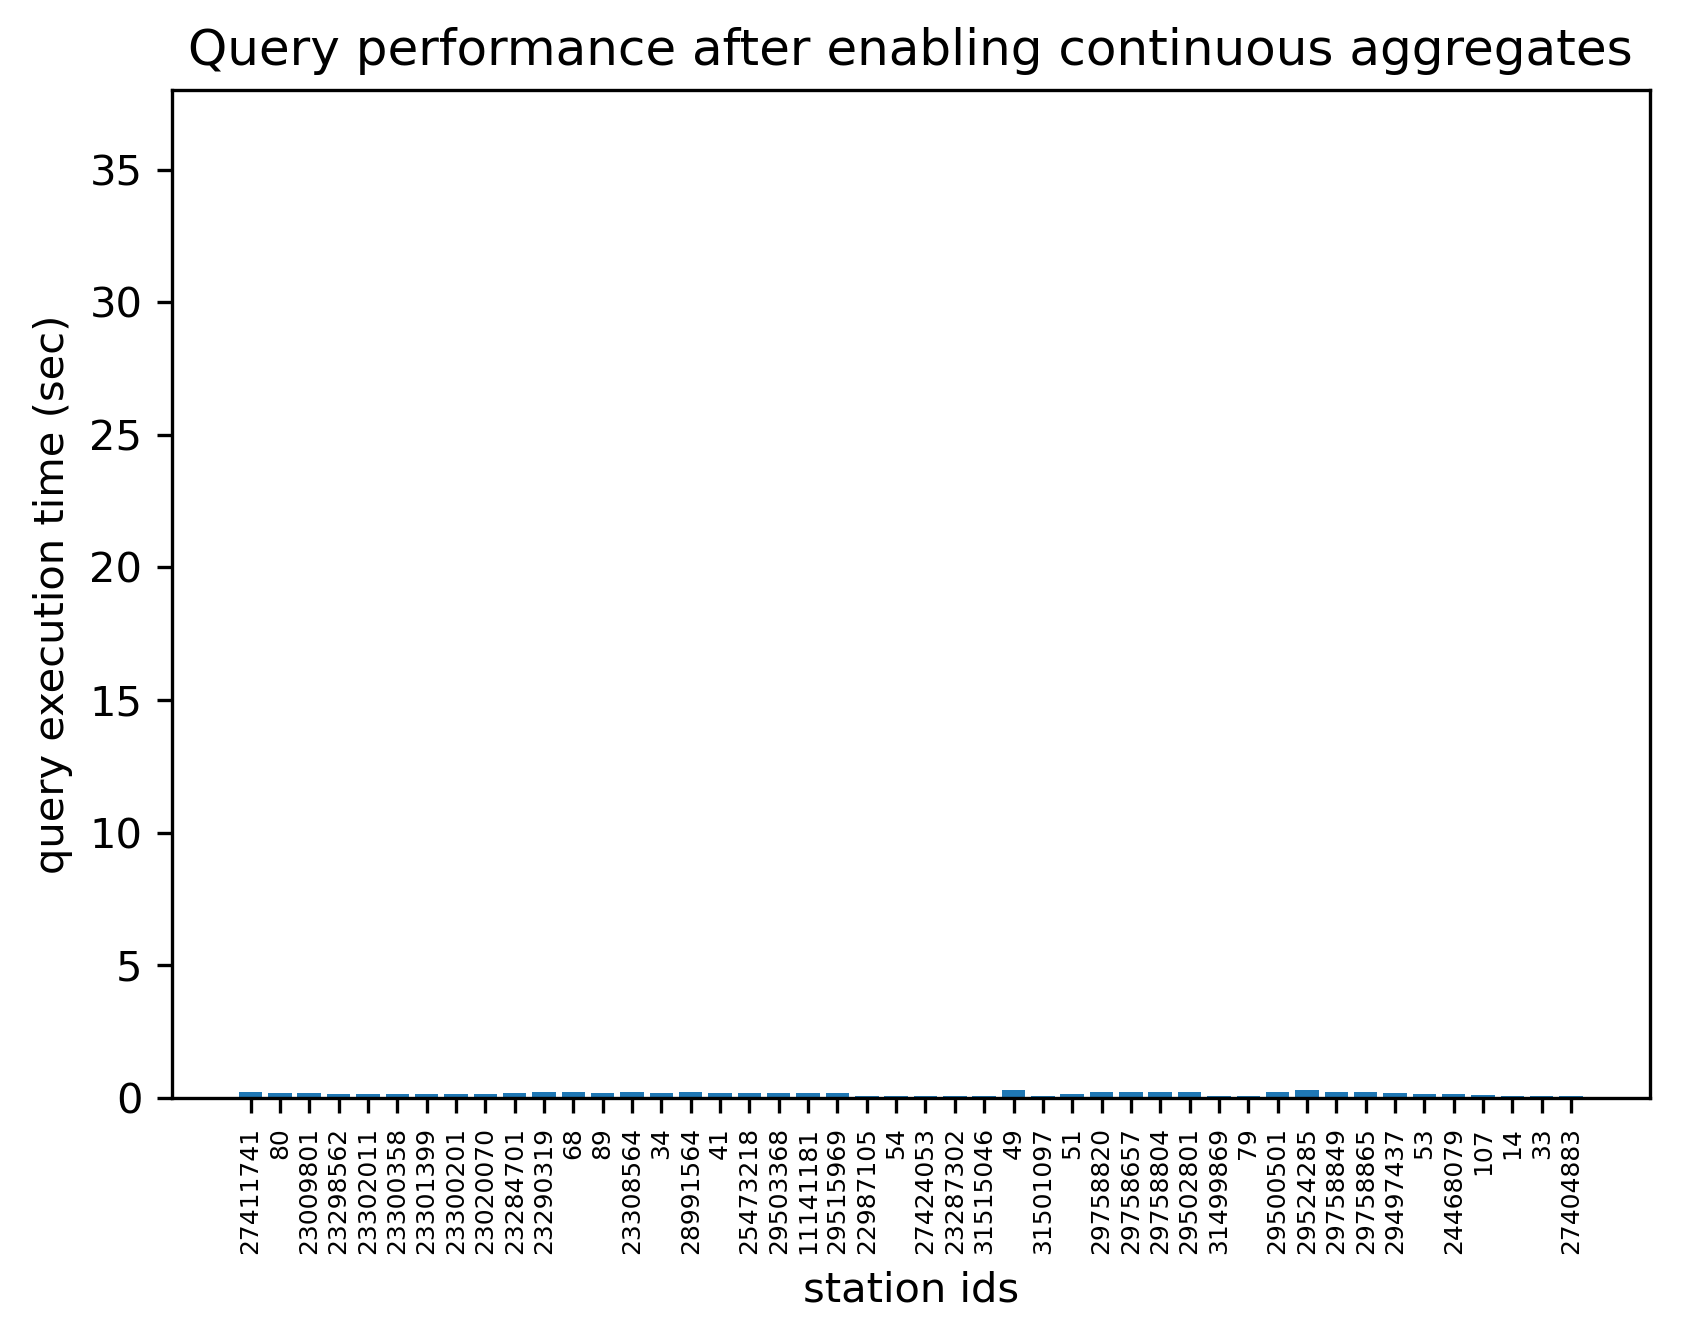
\includegraphics[width=0.85\textwidth,height=\textheight,keepaspectratio]{img/query_dopo}
\caption{Tempi di risposta per query temporali sulle centraline AirQino dopo l'ottimizzazione (media su 10 iterazioni)}
\label{fig:query-dopo}
\end{figure}

Da cui si può notare che con la nuova query, ottimizzata con continuous aggregates, i tempi di risposta risultano costanti per tutte le centraline indipendentemente dalla quantità di dati, garantendo scalabilità ed efficienza.

\chapter{Calibrazione}\label{ch:calibrazione}
% TODO meglio
Questo capitolo riguarda la parte di regressione. Nella sezione \ref{sec:dati} vengono presentati i dataset a disposizione, la loro struttura e il lavoro di preprocessamento.
La sezione \ref{sec:regressione} racchiude una breve panoramica teorica sui concetti di regressione, correlazione, metriche (coefficiente di correlazione, coefficiente di determinazione, scarto quadratico medio), analisi dei residui, modelli di regressione (sia lineare che non lineari).
La sezione \ref{sec:esperimenti} presenta i risultati ottenuti, mentre la sezione \ref{sec:validazione} riassume la parte di validazione.
Infine, la sezione \ref{sec:discussione} riassume 

% I dati a disposizione
\section{I dati a disposizione}\label{sec:dati}
\ldots

\subsection{Dataset NO2}\label{ssec:dataset-no2}
\ldots

\subsection{Dataset PM2.5 e PM10}\label{ssec:dataset-pm}
\ldots

\subsection{Preprocessamento}\label{ssec:preprocessamento}
\ldots

% Regressione
\section{Regressione}\label{sec:regressione}

%La regressione è una tecnica statistica che serve a stimare la relazione esistente tra due o più variabili. In particolare, la regressione permette di individuare il coefficiente di correlazione tra due variabili e di determinare se questa relazione è casuale o no.
%
%Tra le applicazioni principali della regressione ci sono:
%
%- Stima della relazione tra due variabili
%
%- Analisi della relazione tra variabili
%
%- Valutazione dell'influenza di una variabile sulle altre
%
%- Predicting


Nella statistica applicata come nelle scienze sperimentali si osserva (o si ipotizza) l’esistenza di relazioni fra due o più grandezze.

Sorge allora il problema di determinare una funzione che, in base ai dati ricavati mediante esperimenti o rilevazioni statistiche, rappresenti questi relazioni permettendo, in questo modo, di analizzare meglio i fenomeni osservati.

\subsection{Introduzione}\label{ssec:regressione-introduzione}
Limitando lo studio a problemi che stabiliscono relazioni fra due sole variabili, si tratta, partendo dalle coppie $(x_i, y_i)$ di dati corrispondenti rilevati, di determinare una funzione $y=f(x)$ che rappresenti il fenomeno.

Per trovare una funzione che rappresenti il fenomeno si può procedere in due modi:

\begin{itemize}
  \item determinare una funzione che assuma esattamente i valori $(x_i, y_i)$ rilevati; questo procedimento viene detto interpolazione per punti noti;
  \item determinare una funzione che si accosti il più possibile ai punti $(x_i, y_i)$; questo procedimento viene detto interpolazione fra punti noti.
\end{itemize}

La ricerca di una funzione, generalmente espressa da un polinomio, che passi esattamente per i punti $(x_i, y_i)$ è piuttosto laboriosa; nelle applicazioni statistiche si preferisce determinare una funzione il cui grafico si avvicini ai punti rilevati.

Osservando l’andamento del fenomeno si sceglie il tipo di funzione interpolatrice: lineare, quadratica, esponenziale, ecc. e quindi si procede alla determinazione dei parametri, ossia delle costanti che compaiono nella funzione scelta in modo che sia soddisfatta una condizione di accostamento prefissata.

Per conseguire questo scopo il metodo più utilizzato è il metodo dei \textbf{minimi quadrati} che costituisce un’applicazione della ricerca del minimo di una funzione di più variabili mediante gli strumenti dell’analisi infinitesimale.

Si considerino due variabili $X$ e $Y$ sulle quali si sono effettuate $n$ rilevazioni: $$\left(x_{1}, y_{1}\right),\left(x_{2}, y_{2}\right), \ldots,\left(x_{i}, y_{i}\right), \ldots,\left(x_{n}, y_{n}\right)$$

Sia $y=f(x; a, b, c, ..., k)$ la funzione interpolatrice scelta. Siano inoltre $\hat{y}_{i}$ valori predetti sulla curva corrispondenti ai valori $x_i$ rilevati.

La condizione di accostamento data dal metodo dei minimi quadrati è quella di determinare i valori dei parametri in modo che sia minima la somma dei quadrati delle differenze fra i valori osservati $y_i$ e i valori predetti $\hat{y}_i$ (figura \ref{fig:minimi_quadrati}), ovvero:

$$\varphi(a, b, c, \ldots, k)=\sum_{i=1}^{n}\left[y_{i}-f\left(x_{i} ; a, b, c, \ldots, k\right)\right]^{2}$$\smallskip

dove i valori $x_i$ e $y_i$ sono noti, mentre sono incogniti i parametri $a , b , c , … , k$ della funzione. \cite{excel_per_statistica_belluco}

\begin{figure}[H]
\centering
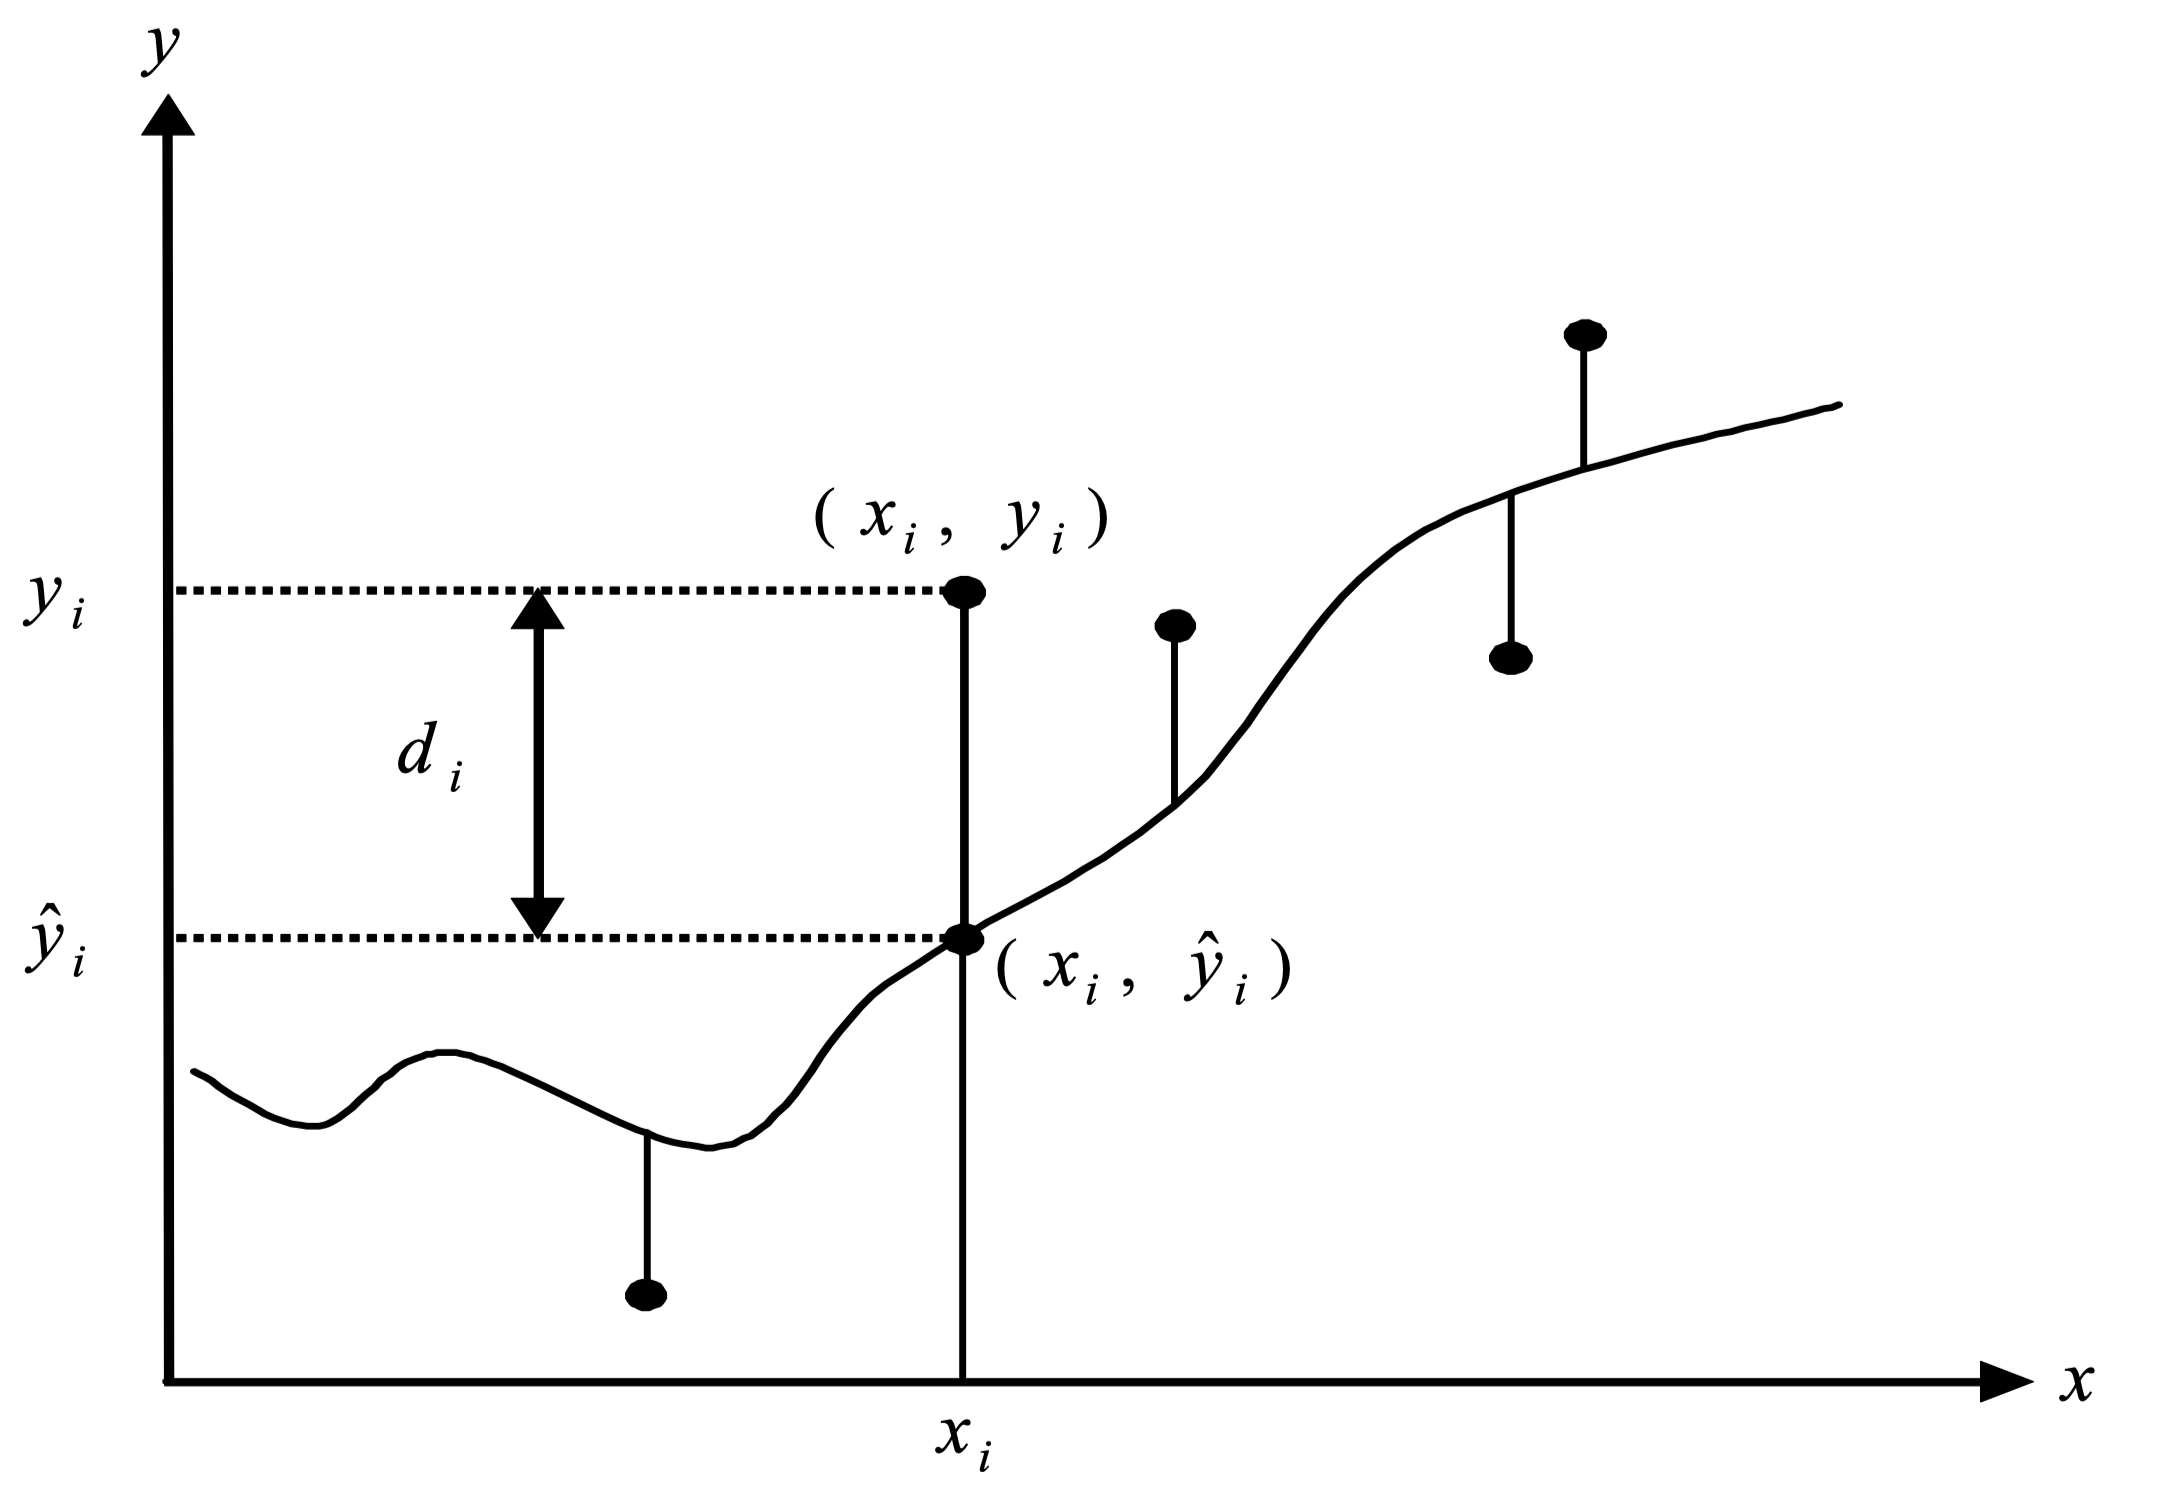
\includegraphics[width=0.75\textwidth,height=\textheight,keepaspectratio]{img/minimi_quadrati.png}
\caption{Condizione dei \textit{minimi quadrati} \cite{excel_per_statistica_belluco}}
\label{fig:minimi_quadrati}
\end{figure}

\subsection{Correlazione e coefficiente di determinazione}\label{ssec:regressione-correlazione}

Quando la dipendenza tra le due variabili è lineare, si parla di correlazione lineare, che può essere valutata mediante il coefficiente di correlazione lineare ($r$):

$$r=\frac{\sum_{i=1}^{n}\left(x_{i}-\bar{x}\right)\left(y_{i}-\bar{y}\right)}{\sqrt{\sum_{i=1}^{n}\left(x_{i}-\bar{x}\right)^{2}} \sqrt{\sum_{i=1}^{n}\left(y_{i}-\bar{y}\right)^{2}}}$$\smallskip

dove il termine al numeratore rappresenta la \textit{covarianza} di $X$ ed $Y$ cioè la variabilità congiunta delle coppie ($x_i$, $y_i$) di valori corrispondenti rispetto al proprio valor medio; mentre il denominatore rappresenta il prodotto delle deviazioni standard di $X$ ed $Y$.

Il coefficiente di correlazione lineare gode di importanti proprietà:

\begin{itemize}
  \item $-1 \le r \le 1$;
  \item si ha $r=1$ quando tutti i dati sono allineati lungo una retta crescente (figura \ref{fig:positive_correlation});
    \begin{figure}[H]
\centering
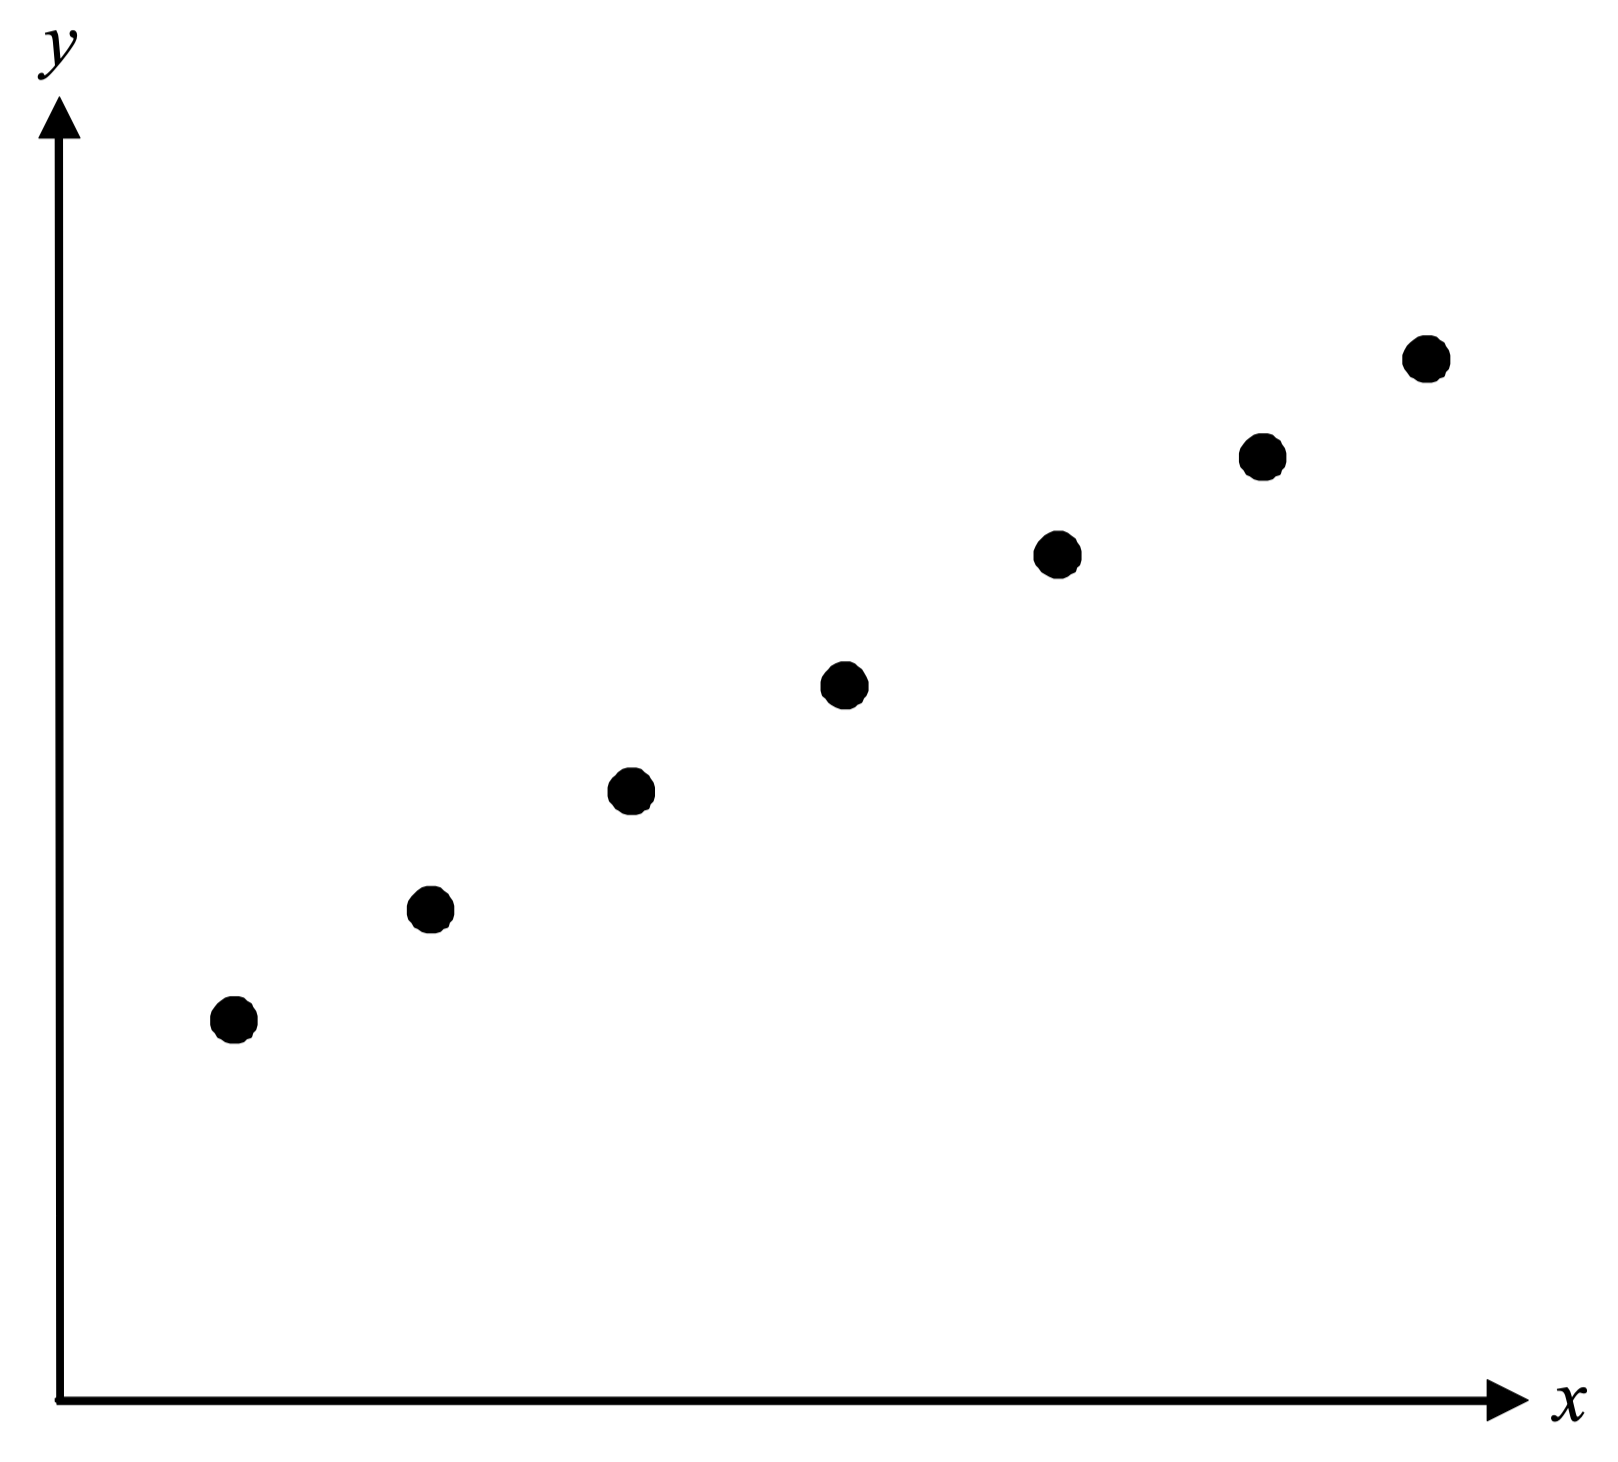
\includegraphics[width=0.55\textwidth,height=\textheight,keepaspectratio]{img/positive_correlation.png}
\caption{Correlazione lineare positiva}
\label{fig:positive_correlation}
\end{figure}

  \item si ha $r=-1$ quando tutti i dati sono allineati lungo una retta decrescente  (figura \ref{fig:negative_correlation});
      \begin{figure}[H]
\centering
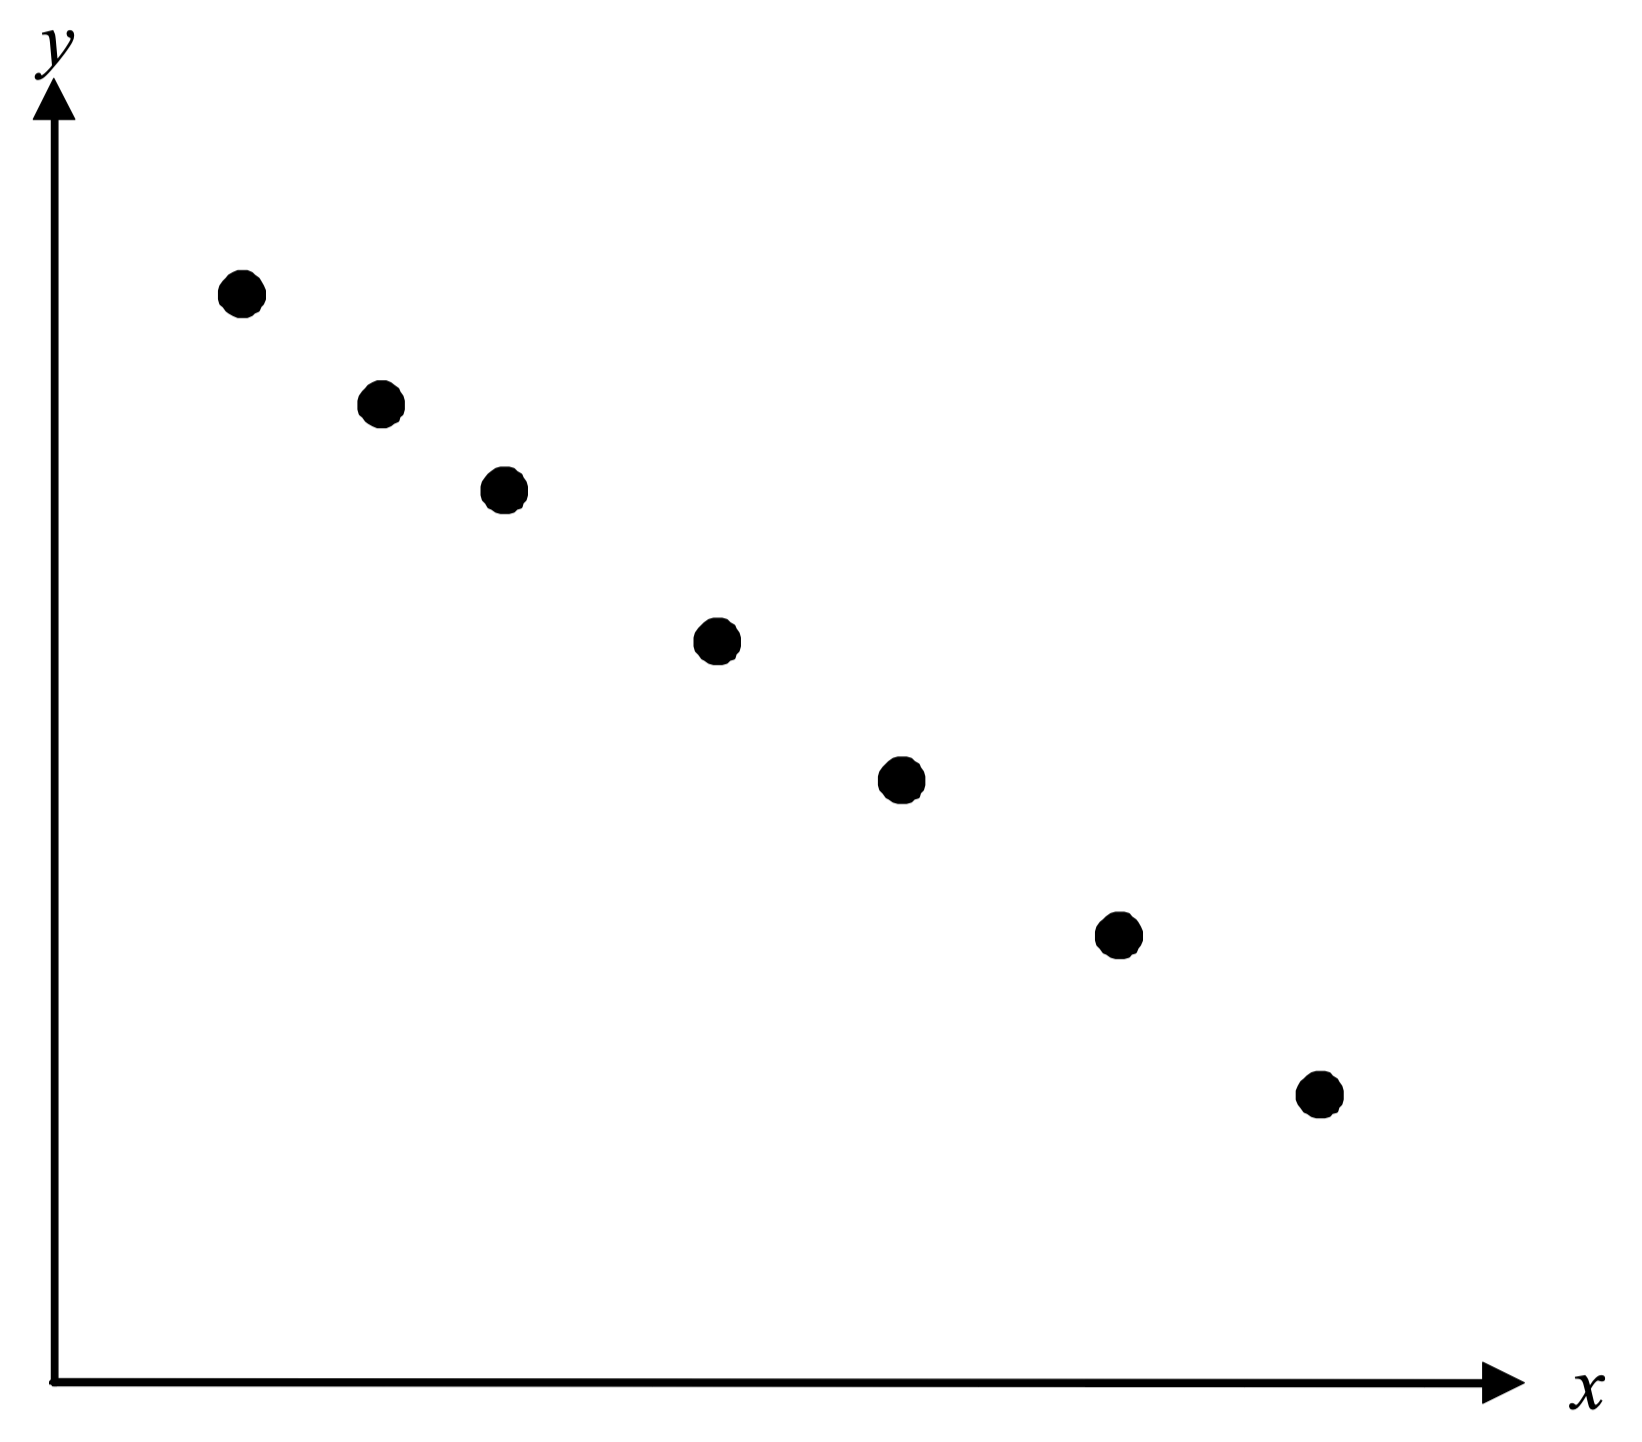
\includegraphics[width=0.55\textwidth,height=\textheight,keepaspectratio]{img/negative_correlation.png}
\caption{Correlazione lineare negativa}
\label{fig:negative_correlation}
\end{figure}
  \item si ha $r=0$ quando non esiste una relazione lineare tra i dati  (figura \ref{fig:no_correlation}).
  \begin{figure}[H]
\centering
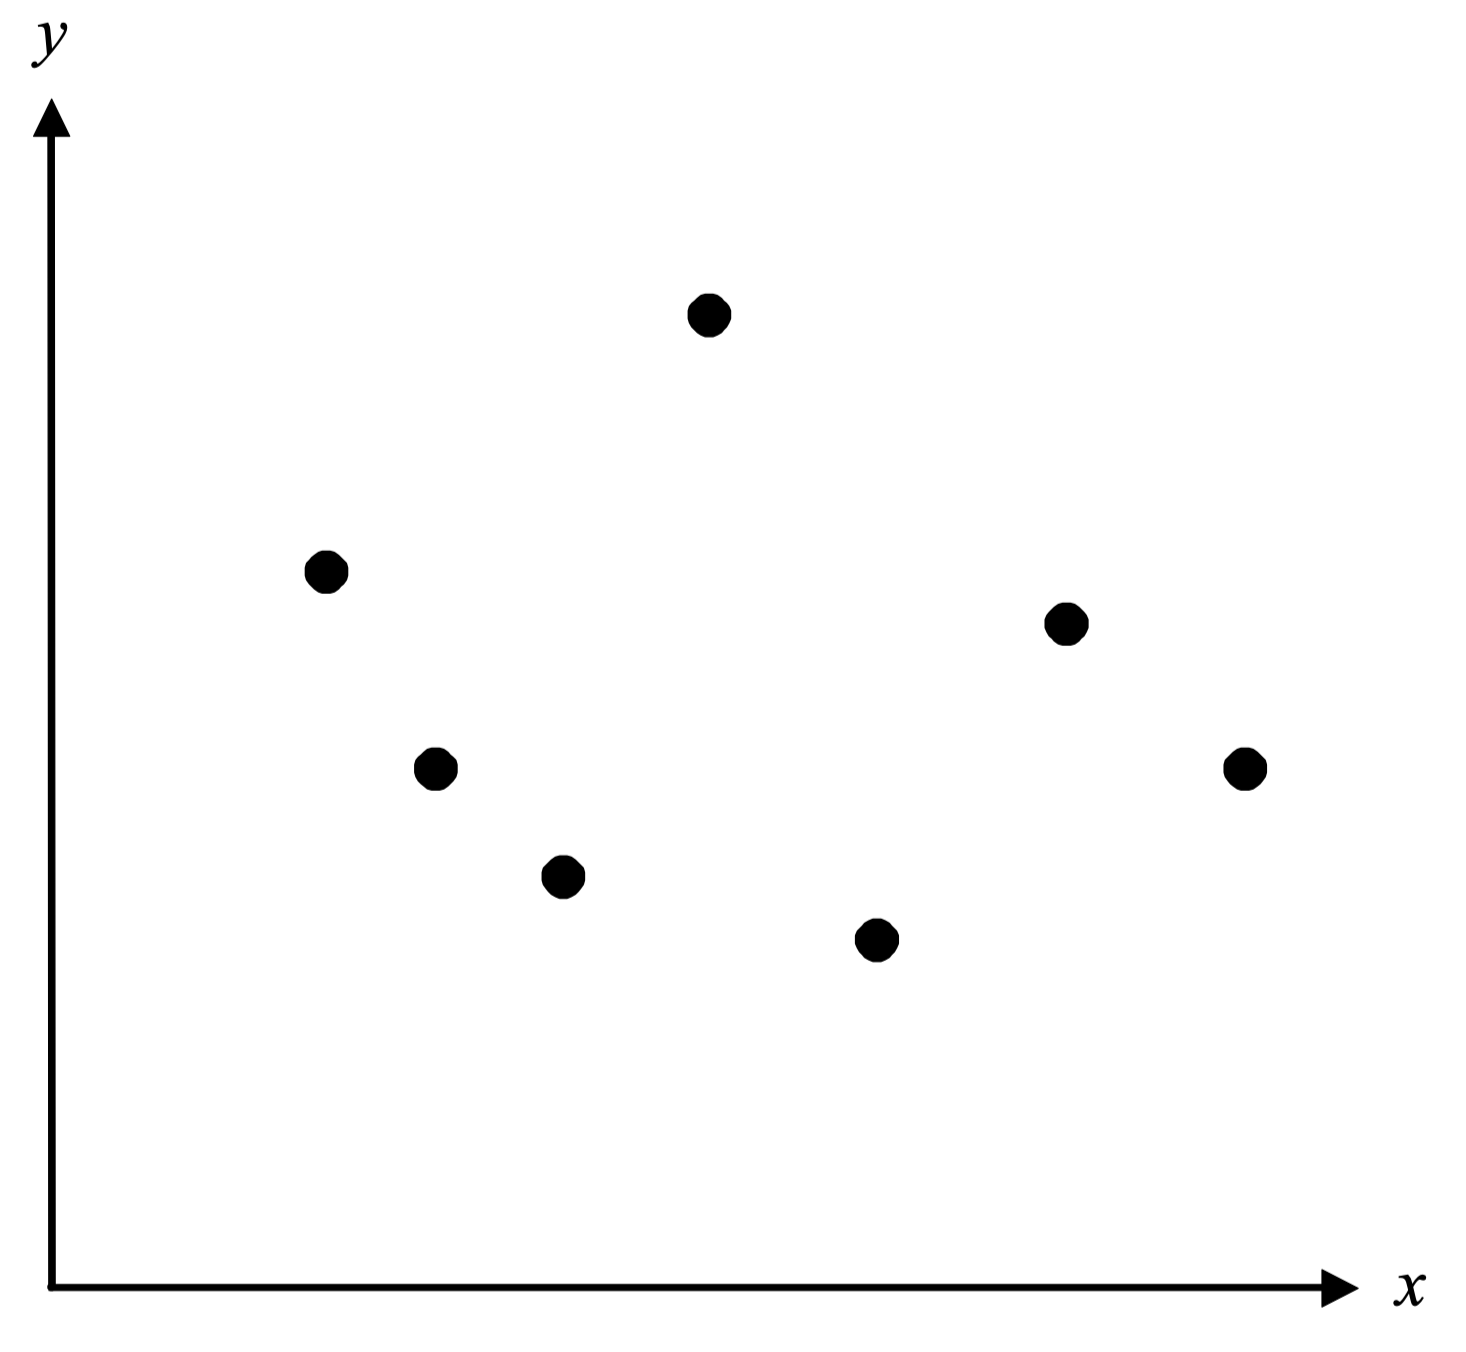
\includegraphics[width=0.55\textwidth,height=\textheight,keepaspectratio]{img/no_correlation.png}
\caption{Nessuna correlazione}
\label{fig:no_correlation}
\end{figure}
\end{itemize}

Sapendo che la varianza ($\sigma_{y}^{2}$) della variabile $Y$ si può scomporre in una parte ($\sigma_{\hat{y}}^{2}$), detta varianza spiegata, in quanto la variabilità della $Y$ è dovuta alla dipendenza di $Y$ dalla variabile $X$, e in una parte ($\sigma_{e}^{2}$), detta varianza non spiegata, in quanto la variabilità della $Y$ non dipende dalla variabile $X$, ma da altri fattori; si può introdurre un secondo indicatore, dato dal rapporto tra la varianza spiegata e la varianza totale, chiamato \textbf{coefficiente di determinazione}:

$$r^{2}=\frac{\sigma_{\hat{y}}^{2}}{\sigma_{y}^{2}}$$\smallskip

che indica quale frazione di varianza totale è dovuta alla dipendenza fra le variabili $Y$ e $X$, ossia quale frazione della variazione della variabile Y è spiegata dalle variazioni della variabile $X$.

Sapendo che:

$$\sigma_{y}^{2}=\sigma_{\hat{y}}^{2}+\sigma_{e}^{2}$$

allora:

$$r^{2}=\frac{\sigma_{\hat{y}}^{2}}{\sigma_{\hat{y}}^{2}+\sigma_{e}^{2}}$$\smallskip

è evidente, quindi, che se la variabilità non spiegata è trascurabile, $\sigma_{e}^{2}$ tende ad annullarsi ed $r^{2}$ avrà un valore prossimo ad 1, mentre diverrà via via minore di 1 al diminuire dell’accordo tra la funzione calcolata e le osservazioni sperimentali.

Minore è la somma residua rispetto alla somma totale dei quadrati, maggiore sarà il valore del coefficiente di determinazione, $r^2$, il quale è un indicatore del livello di precisione con cui l'equazione ottenuta dall'analisi di regressione spiega la relazione tra le variabili. \cite{linear_models}\\

Un'altra metrica utile in ambito delle regressioni è l'errore quadratico medio (in inglese \textit{Mean Squared Error}, MSE) che indica la discrepanza quadratica media fra i valori dei dati osservati ed i valori dei dati stimati:

$$MSE=\frac{\sum_{i=1}^{n}\left(x_{i}-\widehat{x}_{i}\right)^{2}}{n}$$\smallskip

La sua radice quadrata fornisce un ulteriore indice statistico, la cosiddetta radice dell'errore quadratico medio (in inglese \textit{root-mean-square error}, RMSE). L'RMSE può essere anche calcolato come deviazione standard degli scarti. Da notare che l'MSE ed RMSE non sono quantità a-dimensionali, bensì assumono l'unità di misura della grandezza considerata (RMSE) ed il suo quadrato (MSE). 

\subsection{Analisi dei residui}\label{ssec:regressione-residui}
Esistono metodi utili per diagnosticare le violazioni delle ipotesi di regressione di base: questi si basano principalmente sullo studio dei residui del modello. Spesso infatti la retta di regressione è infatti una semplificazione della realtà e non coglie tutta la variabilità presente in un insieme di dati. \cite{residui_pozzolo}

Si definiscono i residui come:

$$e_{i}=y_{i}-\hat{y}_{i}, \quad i=1,2, \ldots, n$$\smallskip

dove $y_{i}$ è il valore osservato e $\hat{y}_{i}$ è il valore predetto.

Poiché un residuo può essere visto come la deviazione tra i dati e l'adattamento, è anche una misura della variabilità nella variabile di risposta non spiegata dal modello di regressione. \cite{introduction_to_lr}

Eventuali scostamenti dalle ipotesi sugli errori dovrebbero quindi manifestarsi nei residui. L'analisi grafica dei residui è un modo efficace per scoprire diversi tipi di inadeguatezze del modello, tra cui: 
\begin{itemize}
  \item se i residui hanno distribuzione normale (\ref{ssec:distr-errori});
  \item se le varibabili indipendenti sono correlate con l'errore (\ref{ssec:correlazione-errore-variabili});
  \item se la varianza dei residui è omogenea (\ref{ssec:omogeneita-varianza});
  \item se ci sono degli outliers che influenzano la pendenza della retta (\ref{ssec:influenza-outliers}).
\end{itemize}

\subsubsection{Distribuzione degli errori}\label{ssec:distr-errori}
La distribuzione normale degli errori può essere verificata attraverso un grafico dei quantili, detto anche q-q plot.
In questa tipologia di grafico, i quantili teorici di una distribuzione Normale sono riportati sull’asse orizzontale. I quantili dei residui standardizzati sono invece riportati sull’asse verticale.
L’idea è che se i residui hanno una distribuzione normale, i loro quantili dovrebbero coincidere con quelli della distribuzione normale. A livello visivo, questo significa che i punti dovrebbero disporsi lungo la \textit{bisettrice}, indicata dalla retta presente nel grafico (figura TODO).

%TODO figura + ref

Nella pratica, non capita quasi mai che i punti si dispongano esattamente lungo la bisettrice. Per poter dire che gli errori hanno una distribuzione normale ci si accontenta quindi che i punti siano vicino alla linea presente nel grafico.
Tuttavia in generale le stime sui coefficienti di regressione sono abbastanza robuste a violazioni della normalità distributiva dei residui.

\subsubsection{Correlazione tra errore e variabili}\label{ssec:correlazione-errore-variabili}
Se una variabile esplicativa è correlata con il termine d’errore, è possibile utilizzare questa variabile esplicativa per predire quale sarà l’errore del modello di regressione. Questo in generale non è un buon segno, perché la componente di errore di un modello di previsione deve essere imprevedibile.

Per verificare la non correlazione tra la variabile indipendente (x) e i residui è utile osservare un grafico di dispersione come quello riportato in figura TODO, in sull’asse orizzontale si mettono i valori della x, mentre sull’asse verticale i valori dei residui.

%TODO figura + ref

L’ipotesi è confermata se non è individuabile nessuna relazione tra le due variabili.

\subsubsection{Omogeneità della varianza dei residui}\label{ssec:omogeneita-varianza}
Per verificare l’ipotesi di omogeneità delle varianze dei residui, è necessario creare un grafico a dispersione.  I valori stimati della y si riportano sull’asse orizzontale delle x. Sull’asse verticale delle y invece si indicano i valori dei residui (figura \ref{fig:distr_residui}).

\begin{figure}[H]
\centering
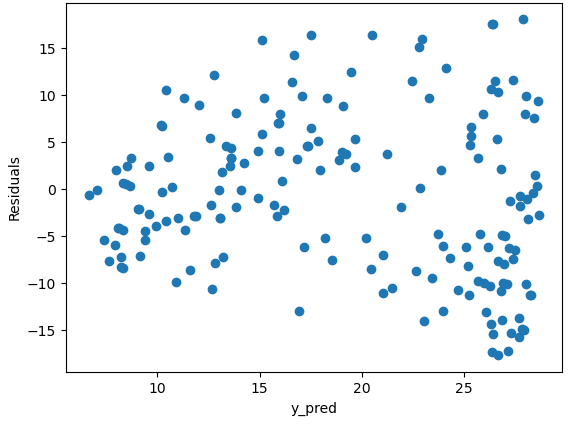
\includegraphics[width=0.65\textwidth,height=\textheight,keepaspectratio]{img/distr_residui.png}
\caption{Esempio di distribuzione dei residui}
\label{fig:distr_residui}
\end{figure}

Se c’è omogeneità della varianza dei residui, i punti saranno dispersi in modo simile sia nella parte sinistra che in quella destra del grafico. Questa proprietà se verificata prende il nome di \textbf{omoschedasticità}.

\subsubsection{Influenza di outliers}\label{ssec:influenza-outliers}
Il grafico a dispersione tra valori predetti e residui permette di individuare anche i possibili outliers, ovvero i punti isolati nel grafico (quelli con residui maggiori).
Tuttavia, per verificare se ci sono outliers in un modello di regressione, spesso si utilizzano altre tecniche (ad esempio eliminando i punti problematici tramite la distanza di Cook, descritta in \ref{sssec:regressione-cook}, oppure applicando stime robuste meno sensibili alle le osservazioni problematiche, ad esempio con la funzione peso di Huber  descritta in \ref{sssec:regressione-huber}). Nel primo caso è utile anche provare a rifare le analisi di regressione escludendo le osservazioni potenzialmente problematiche e vedere se ci sono differenze nei coefficienti del modello.

Nei modelli di regressione infatti anche un singolo outlier può influenzare in maniera sostanziale la capacità di adattamento del modello ai dati, soprattutto se il campione non è molto numeroso.

\subsection{Modelli di regressione}\label{ssec:regressione-modelli}
I modelli di regressione sono ampiamente utilizzati sia per la previsione o la descrizione dei dati che la stima e il controllo dei parametri.

\subsubsection{Regressione lineare}\label{sssec:regressione-lineare}
Si considera una funzione lineare a due variabili:
$$y = a + b*x$$

In questo caso si deve rendere minima la funzione:

$$\varphi(a, b)=\sum_{i=1}^{n}\left[y_{i}-\left(a+b x_{i}\right)\right]^{2}$$\smallskip

Annullando le derivate parziali prime rispetto ad $a$ e $b$ si ha il sistema:

$$\left\{\begin{array}{l}
\sum_{i=1}^{n} 2\left[y_{i}-\left(a+b x_{i}\right)\right](-1)=0 \\
\sum_{i=1}^{n} 2\left[y_{i}-\left(a+b x_{i}\right)\right]\left(-x_{i}\right)=0
\end{array}\right.$$\smallskip

che risolto, fornisce i valori dei parametri:

$$\left\{\begin{array}{l}
\hat{a}=\bar{y}-b \bar{x} \\
\hat{b}=\frac{\sum_{i=1}^{n}\left(x_{i}-\bar{x}\right)\left(y_{i}-\bar{y}\right)}{\sum_{i=1}^{n}\left(x_{i}-\bar{x}\right)^{2}}
\end{array}\right.$$\smallskip

dove $\bar{x}$ e $\bar{y}$ indicano le \textit{medie aritmetiche}, rispettivamente di $x_i$ e $y_i$.

La stima del parametro $b$, \textit{coefficiente angolare} della funzione lineare, può essere rappresentato nella forma:

$$\hat{b}=\frac{\sum_{i=1}^{n} \frac{\left(x_{i}-\bar{x}\right)\left(y_{i}-\bar{y}\right)}{n}}{\sum_{i=1}^{n} \frac{\left(x_{i}-\bar{x}\right)^{2}}{n}}$$\smallskip

dove il denominatore è la \textit{varianza} di $X$ ($\sigma_{X}^{2}$), mentre il numeratore è detto \textit{covarianza} di X e Y ($\sigma_{XY}$) e misura la variabilità congiunta delle coppie ($x_i$, $y_i$) di valori corrispondenti rispetto al proprio valor medio; quindi, il coefficiente $b$ della retta interpolante esprime la variabilità congiunta di $X$ e $Y$ rapportata alla variabilità della sola $X$.

\begin{figure}[H]
\centering
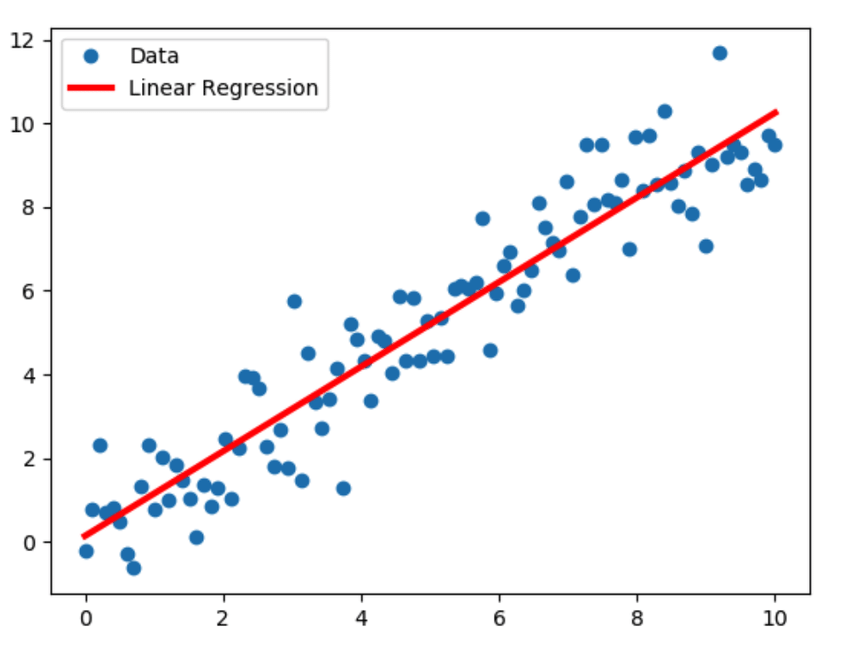
\includegraphics[width=0.65\textwidth,height=\textheight,keepaspectratio]{img/lin_reg_example.png}
\caption{Esempio di regressione lineare}
\label{fig:reg_lin}
\end{figure}

La precisione della retta calcolata dalla regressione lineare dipende dal grado di dispersione nei dati. Più i dati sono lineari, più il modello risulterà accurato.

%Per stimare la relazione tra due variabili, la regressione lineare utilizza una formula matematica che calcola la media dei valori della prima variabile (Y) in funzione dei valori della seconda variabile (X). La formula della regressione lineare è:
%
%Y = a + bX
%
%In questa formula, a è la costante di regressione e b è la coefficiente di regressione. La costante di regressione a indica la media dei valori di Y in funzione dei valori di X. Il coefficiente di regressione b indica la relazione tra le due variabili: più è vicino a 1, più le due variabili sono correlate in modo lineare.
%
%Utilizzando la regressione lineare, è possibile stimare la relazione tra due variabili anche in presenza di deviazioni dalla linea.

\subsubsection{Regressione lineare robusta (Huber)}\label{sssec:regressione-huber}
La regressione Huber (in inglese Huber regression, anche detta regressione robusta) è una metodologia statistica per la stima dei parametri di un modello lineare in presenza di \textit{outliers}.

Ci sono situazioni in cui si verifica presenza di valori anomali che influiscono sul modello di regressione, nel senso che possono avere una forte influenza sul metodo dei minimi quadrati, di fatto \textit{deviando} troppo l'equazione di regressione nella loro direzione. Il metodo dei minimi quadrati, infatti, in questi casi ha lo svantaggio di avere la tenedenza a essere dominato da questi valori — infatti sommando il quadrato dei residui ($\sum_{i=1}^{n} a_i^2$ dove $a_i$ è il residuo i-esimo), la media risulta troppo influenzata da pochi valori $a_i$ particolarmente grandi.

Ci sono due modi per affrontare questa situazione:

\begin{itemize}
  \item Scartare le osservazioni \textit{scomode} (vedi regressione lineare avanzata \ref{sssec:regressione-cook});
  \item Applicare procedure di stime robuste in modo che siano meno sensibili alle osservazioni troppo influenti (figura \ref{fig:reg_rob}).
\end{itemize}

\begin{figure}[H]
\centering
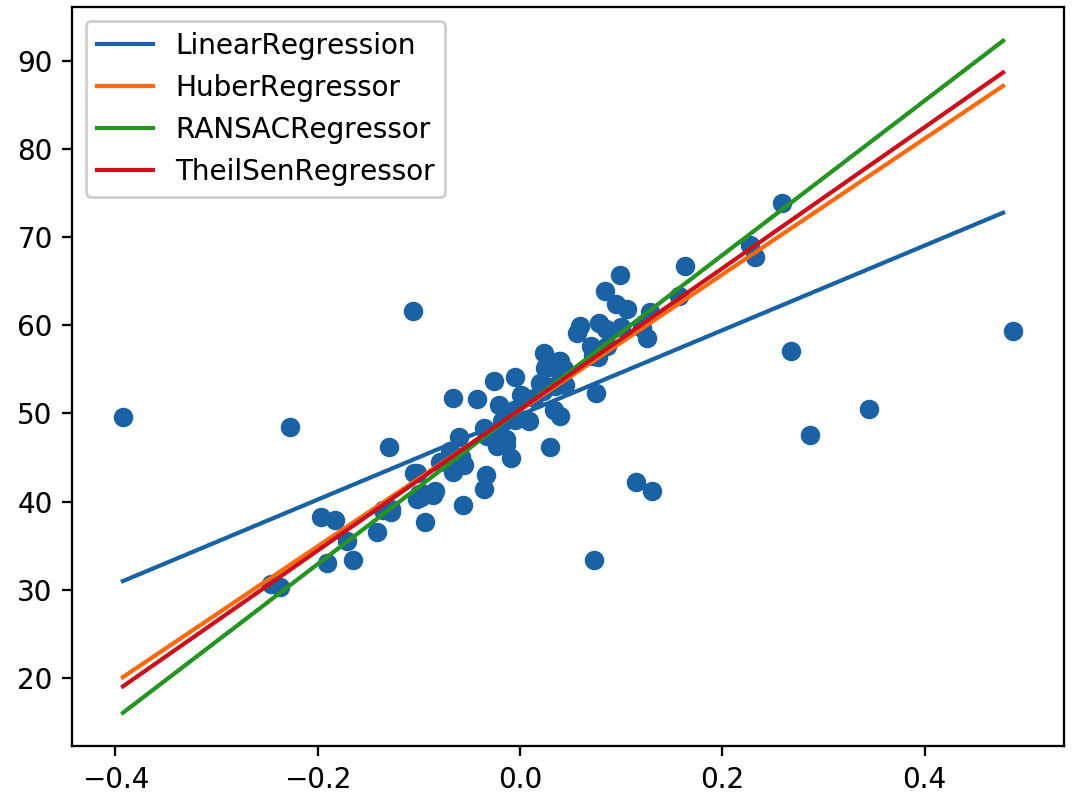
\includegraphics[width=0.65\textwidth,height=\textheight,keepaspectratio]{img/robust.png}
\caption{Comportamento di modelli di regressione robusta in presenza di outliers}
\label{fig:reg_rob}
\end{figure}

Una delle funzioni di stima robusta, comunemente usata in diversi metodi di regressione per ridurre la sensibilità dei parametri alla presenza di outliers, è la \textbf{funzione di Huber}, che risulta quadratica per piccoli valori di $x$, e lineare per valori più grandi. È definita come:

$$L_{\delta}(a)= \begin{cases}\frac{1}{2} a^{2} & \text { per }|a| \leq \delta \\ \delta\left(|a|-\frac{1}{2} \delta\right), & \text { altrimenti }\end{cases}$$\smallskip

Dove la variabile $a$ fa riferimento al residuo, cioè la differenza tra valore osservato e valore predetto ($a = y - f(x)$).


\subsubsection{Regressione lineare avanzata}\label{sssec:regressione-cook}
Come accennato in \ref{sssec:regressione-huber}, un'altra tecnica per la gestione di outlier è quella di applicare il modello sul dataset dopo aver rimosso i valori anomali. Esistono molte metriche su cui basarsi per rimuovere gli outlier da un set di dati: un metodo che viene spesso utilizzato nella regressione è la \textbf{distanza di Cook}.

La distanza di Cook è una stima dell'\textit{influenza} di una osservazione in un dataset, in termini di residuo (outlier) o di elevato \textit{leverage}: è un riepilogo di quanto cambierebbe un modello di regressione nel caso in cui venga rimossa l'i-esima osservazione.

In presenza di outliers la distanza di Cook aumenta, e quindi questi dati ad alta influenza hanno un maggiore impatto sulle stime dei parametri della regressione.

La distanza di Cook \cite{cook_def} dell'osservazione $i$ ($\forall i=1, \ldots, n$) è definita come:

$$D_{i}=\frac{\sum_{j=1}^{n}\left(\hat{y}_{j}-\hat{y}_{j(i)}\right)^{2}}{p s^{2}}$$\smallskip

dove:

\begin{itemize}
  \item $n$ è il numero di osservazioni;
  \item $\hat{y}_{j}$ è il valore predetto;
  \item $\hat{y}_{j(i)}$ è la risposta ottenuta escludendo l'i-esima osservazione.
\end{itemize}

Oppure, in modo equivalente:

$$D_{i}=\frac{e_{i}^2}{p s^{2}}\left[\frac{h_{i}}{\left(1-h_{i}\right)^{2}}\right]$$\smallskip

dove:

\begin{itemize}
  \item $e_{i} = y_i - \hat{y_i}$  è l'i-esimo residuo;
  \item $p$ è il numero di coefficienti della regressione;
  \item $s^2$ è l'errore quadratico medio (MSE);
  \item $h_i$ è il peso che l'i-esimo osservazione ha sul valore della regressione (\textit{leverage}).
\end{itemize}

Un esempio di rilevazione grafica di outlier tramite distanza di Cook è riportato in figura \ref{fig:cook}.

\begin{figure}[H]
\centering
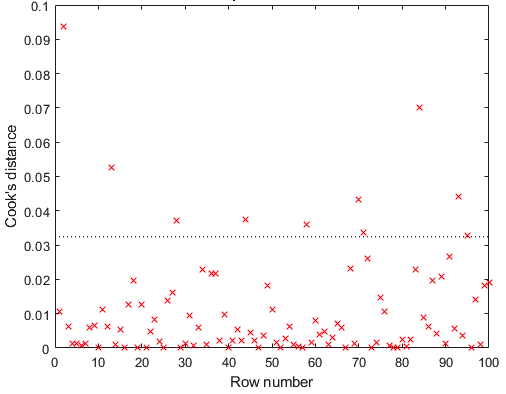
\includegraphics[width=0.65\textwidth,height=\textheight,keepaspectratio]{img/cook.png}
\caption{Riconoscimento di outlier tramite distanza di Cook}
\label{fig:cook}
\end{figure}

Vi sono diverse opinioni riguardo al valore di soglia di \textit{cut-off}, oltre la quale un dato può essere considerato un outlier. In \cite{applied_regression} viene proposta:

$$D_{i}>\frac{4}{n}$$\smallskip

dove $n$ è il numero di osservazioni. La distanza di Cook può anche essere utilizzata per individuare regioni dello spazio nelle quali sarebbe necessario effettuare una validazione, ad esempio acquisendo più dati.

\subsubsection{Regressione Ridge}\label{sssec:regressione-ridge}
Nella statistica e nel Machine Learning, la regressione Ridge è un metodo di analisi di regressione che applica una fase di \textbf{regolarizzazione} al fine di migliorare l'accuratezza della previsione, prevenire l'\textit{overfitting} e penalizzare la complessità del modello.
Insieme al LASSO (vedi \ref{sssec:regressione-lasso}) è un modello di regressione che viene ripreso anche da tecniche di Boosting di Machine Learning.

Parlando di regolarizzazione in generale esistono due tipi di penalizzazione:
\begin{itemize}
  \item \textbf{L1}: penalizza il valore assoluto dei coefficienti del modello (es. Lasso); 
  \item \textbf{L2}: penalizza il quadrato del valore dei coefficienti del modello (es. Ridge).
\end{itemize}

La regressione Ridge usa la penalità L2: in pratica questo produce coefficienti piccoli, ma nessuno di loro è mai annullato (\textit{feature shrinkage}).

Richiamando il metodo dei minimi quadrati (\ref{ssec:regressione-introduzione}) si deve minimizzare la somma dei quadrati dei residui (RSS):

$$\mathrm{RSS}=\sum_{i=1}^{n}\left(y_{i}-\beta_{0}-\sum_{j=1}^{p} \beta_{j} x_{i j}\right)^{2}$$\smallskip

Nella regressione Ridge si aggiunge anche un termine di penalità, ottenendo quindi:

$$\sum_{i=1}^{n}\left(y_{i}-\beta_{0}-\sum_{j=1}^{p} \beta_{j} x_{i j}\right)^{2}+\lambda \sum_{j=1}^{p} \beta_{j}^{2}=R S S+\lambda \sum_{j=1}^{p} \beta_{j}^{2}$$\smallskip

Dove $\lambda$ è un parametro di \textit{tuning} che serve proprio a controllare l’effetto della penalità: un valore $\lambda=0$ infatti non avrà effetto sul risultato finale (l’equazione viene ricondotta a quella dei minimi quadrati), al contrario per $\lambda \to \infty$ invece i coefficienti di regressione stimati tenderanno a zero poiché si darà molto peso alla penalità del modello. \cite{lasso_vs_ridge}

Il modello di Ridge Regression presenta dei vantaggi rispetto a quello dei minimi quadrati, soprattutto per quanto riguarda il \textit{bias-variance trade-off}: in generale, quando c’è una relazione lineare tra i predittori e la variabile risposta, il modello dei minimi quadrati comporta poco bias ma alta varianza. Questo si traduce nel fatto che una piccola variazione nel training data può generare un cambiamento notevole nei coefficienti stimati; di contro la Ridge regressione lavora bene nelle situazioni dove il modello dei minimi quadrati genera ampia varianza nelle stime.\cite{tesi_polito}

\subsubsection{Regressione Lasso}\label{sssec:regressione-lasso}
Lo svantaggio della regressione Ridge è il fatto di considerare tutte le variabili per la predizione nel modello finale. Il termine di regolarizzazione $\lambda \sum_{j=1}^{p} \beta_{j}^{2}$ tende ad assegnare ai coefficienti valori vicini allo zero, ma non perfettamente zero, a meno che $\lambda = 0$.
Questo non crea problemi per l’ accuratezza della predizione quanto per l’interpretazione delle varabili, soprattutto quando il numero delle variabili diventa alto.

La regressione Lasso (acronimo di \textit{least absolute shrinkage and selection operator}, ovvero operatore di restringimento e selezione minimo assoluto) è un’alternativa alla regressione ridge utilizzata proprio per superare questo problema. L'unica differenza sta nel termine di regolarizzazione, ovvero:

$$\lambda \sum_{j=1}^{p}\left|\beta_{j}\right|$$\smallskip

Per cui l'equazione del modello diventa:

$$\sum_{i=1}^{n}\left(y_{i}-\beta_{0}-\sum_{j=1}^{p} \beta_{j} x_{i j}\right)^{2}+\lambda \sum_{j=1}^{p}\left|\beta_{j}\right|=R S S+\lambda \sum_{j=1}^{p}\left|\beta_{j}\right|$$\smallskip

Anche nel caso di Lasso regression il parametro di regolarizzazione tende a stimare i valori dei coefficienti verso lo zero ma, a differenza della regressione ridge, la penalità $\lambda \sum_{j=1}^{p}\left|\beta_{j}\right|$ costringe uno o più coefficienti ad essere esattamente zero per certi valori di $\lambda$. \cite{tesi_polito}

\subsubsection{Regressione polinomiale}\label{sssec:regressione-polinomiale}
La regressione polinomiale è una generalizzazione della regressione lineare, infatti utilizza lo stesso metodo matematico della variante lineare, ma assume che la relazione di funzione che caratterizza i dati sia meglio descritta, anzichè da una retta, da un polinomio. In questo caso il metodo dei minimi quadrati può essere utilizzato anche per adattare una funzione polinomiale a un insieme di dati. Considerato un polinomio di grado $k$:

$$y=a_{0}+a_{1} x+a_{2} x^{2}+a_{3} x^{3}+\ldots+a_{k} x^{k}$$\smallskip

In questo caso il sistema di equazioni da risolvere è:

$$\left\{\begin{array}{l}
n a_{0}+a_{1} \sum_{i=1}^{n} x_{i}+a_{2} \sum_{i=1}^{n} x_{i}^{2}+\cdots+a_{k} \sum_{i=1}^{n} x_{i}^{k}=\sum_{i=1}^{n} y_{i} \\
a_{1} \sum_{i=1}^{n} x_{i}+a_{2} \sum_{i=1}^{n} x_{i}^{2}+\cdots+a_{k} \sum_{i=1}^{n} x_{i}^{k}=\sum_{i=1}^{n} x_{i} y_{i} \\
\cdots \\
a_{1} \sum_{i=1}^{n} x_{i}^{k}+a_{2} \sum_{i=1}^{n} x_{i}^{k+1}+\cdots+a_{k} \sum_{i=1}^{n} x_{i}^{2 k}=\sum_{i=1}^{n} x_{i}^{k} y_{i}
\end{array}\right.$$\smallskip

che, risolto, permette di ricavare i parametri $a_0$, $a_1$, $a_2$, ..., $a_k$.

I polinomi sono ampiamente utilizzati in situazioni in cui la risposta è curvilinea, poiché anche relazioni non lineari complesse possono essere adeguatamente modellate da polinomi su intervalli ragionevolmente piccoli delle $x$.

\begin{figure}[H]
\centering
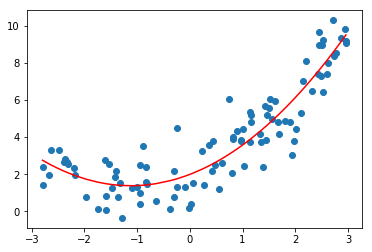
\includegraphics[width=0.65\textwidth,height=\textheight,keepaspectratio]{img/poly_reg_example.png}
\caption{Esempio di regressione polinomiale}
\label{fig:poly_reg}
\end{figure}

Ci sono diverse considerazioni importanti che emergono quando si adatta un polinomio in una variabile: una di queste riguarda la scelta dell'ordine del modello.
Come regola generale, l'uso di polinomi di ordine elevato ($k > 2$) dovrebbe essere evitato: un modello di ordine basso è quasi sempre preferibile a un modello di ordine elevato per ragioni di minore complessità, di coerenza con i dati e per evitare \textit{overfitting}.

Come caso estremo, è sempre possibile trovare un polinomio di grado $n-1$ ad $n$ punti che risulti in un buon adattamento dei dati.
Nella maggior parte dei casi, però, questo non farebbe nulla per migliorare la comprensione della funzione sconosciuta, né sarà probabilmente un buon predittore.

\subsubsection{Regressione con Random Forest}\label{sssec:regressione-rf}
La regressione Random Forest è un algoritmo di apprendimento supervisionato che utilizza il metodo di apprendimento \textit{ensemble} per la regressione tramite alberi di decisione. Il metodo di apprendimento ensemble è una tecnica che combina le previsioni di più algoritmi di apprendimento automatico per effettuare una previsione più accurata rispetto a un singolo modello. \cite{random_forest}

In particolare, una foresta casuale (random forest) opera adattando una serie di alberi decisionali su vari sottocampioni del set di dati e utilizza la media dei risultati per migliorare l'accuratezza predittiva e controllare l'overfitting.
In breve, l'algoritmo funziona esegue i seguenti passi:

\begin{enumerate}
  \item Sceglie a caso $k$ osservazioni dati dal training set;
  \item Costruisce un albero decisionale associato a queste $k$ osservazioni;
  \item Sceglie il numero $N$ di alberi da costruire e ripete i passaggi 1 e 2 per ciascuno;
  \item Per una nuova osservazione, fa in modo che ciascuno degli $N$ alberi preveda il valore di $y$, e assegna il nuovo punto alla media su tutti i valori $y$ previsti.
\end{enumerate}

Uno dei principali svantaggi degli alberi decisionali è che sono molto inclini a fare \textit{overfitting}: funzionano bene sui dati di training, ma non sono così flessibili per fare previsioni su campioni invisibili. Sebbene ci siano soluzioni alternative per questo, come ad esempio ridurre gli alberi, questo riduce il loro potere predittivo. Generalmente sono modelli con bias medio e varianza alta, ma sono semplici e di facile interpretazione.

\subsubsection{Regressione con Gradient Boosting}\label{sssec:regressione-gb}
Il Gradient Boosting è una tecnica di Machine Learning che ha alla base la stima iterativa di alberi sui residui ottenuti ad ogni passo e l’aggiornamento in maniera adattiva delle stime. Questa tecnica riprende il concetto matematico del \textit{Gradient Descent}, per cui lo split scelto sarà quello che favorisce l’avvicinamento al punto di minimo della funzione obiettivo.

Il Gradient Descent è un algoritmo di ottimizzazione che consente di individuare il valore minimo di una funzione di costo per sviluppare un modello con una previsione accurata.

L’algoritmo Gradient Boosting applicato a problemi di regressione può essere descritto nei seguenti passi:

\begin{enumerate}
  \item Si inizializza il modello con un valore noto;
  \item Si considera sul training set una \textit{loss function}, ovvero una funzione differenziabile che esprima una valutazione della predizione (es. $\frac{1}{2} (y_i - \hat{y}_{i})$ dove $y_i$ è l'osservazione e $\hat{y}_{i}$ è la predizione);
  \item Scelto un numero massimo, si itera modellando un albero di regressione seguendo una procedura di discesa del gradiente, in modo da minimizzare la \textit{loss function}. L'albero ottenuto viene aggiunto alla sequenza di alberi già esistente, nel tentativo di correggere o migliorare l'output finale del modello.
\end{enumerate}


\subsubsection{Regressione con SVR}\label{sssec:regressione-svr}
Un altro modello per la regressione è SVR (\textit{support-vector regression}), basato sui modelli SVM (support-vector machines) di apprendimento supervisionato spesso utilizzati per il problema della classificazione. \cite{svm}

Rispetto alla regressione lineare e al metodo dei minimi quadrati, SVR presenta più flessibilità perchè consente di definire una soglia di accettazione dell'errore nel modello. Infatti l'agoritmo SVR si propone di minimizzare non l'errore quadratico, come nel metodo dei minimi quadrati, ma i coefficienti (nello specifico, la norma al quadrato del vettore dei coefficienti). La funzione obiettivo quindi diventa:

$$min \frac{1}{2}\|\mathbf{w}\|^{2}$$\smallskip

 Il termine di errore invece è gestito nei vincoli, dove si imposta l'errore assoluto minore o uguale a un margine specificato, chiamato errore massimo ($\varepsilon$):
 
 $$\left|y_{i}-w_{i} x_{i}\right| \leq \varepsilon$$\smallskip
 
 Il tuning del parametro $\varepsilon$ consente di ottenere la precisione desiderata del modello di regressione. Solitamente alla funzione obiettivo si aggiunge anche delle variabili di \textit{slack} ($\xi_{i}$), che indicano la deviazione dal margine di ciascun valore che supera la soglia $\varepsilon$ (lo scopo è di minimizzarle il più possibile). La funzione obiettivo in questo caso diventa:
 
 $$min \frac{1}{2}\|\mathbf{w}\|^{2} + C \sum_{i=1}^{n}\left|\xi_{i}\right|$$\smallskip

dove $C$ è un altro iperparametro regolabile: all'aumentare di $C$, aumenta anche la tolleranza per i punti al di fuori di $\varepsilon$. Quando invece $C$ si avvicina a 0, la tolleranza si avvicina a 0 e l'equazione ricade nel caso semplificato.

I modelli di regressione SVM possono anche eseguire una regressione non lineare, applicando il \textit{kernel trick} per mappare i dati in uno spazio di caratteristiche multidimensionale. Il tipo di kernel da usare nell'algoritmo è un altro parametro da definire nel modello. I kernel più comuni sono quello lineare, polinomiale (di grado $n$) o rbf (basato su \textit{funzione di base radiale}).

\subsubsection{Regressione con KernelRidge}\label{sssec:regressione-kridge}
La regressione Kernel Ridge (o KRR, \textit{Kernel Ridge Regression}) è un altro modello che combina la regressione Ridge (descritta in \ref{sssec:regressione-ridge}) con il \textit{kernel trick}, imparando così una funzione lineare nello spazio indotto dal rispettivo kernel e dai dati. Per i kernel non lineari, questo corrisponde a una funzione non lineare nello spazio originale. \cite{krr}

La forma del modello di regressione KRR è identica a quello basato su SVR (descritto in \ref{sssec:regressione-svr}), ma vengono utilizzate diverse funzioni di \textit{loss}: KRR minimizza l'errore quadratico mentre SVR minimizza i coefficienti in base alla soglia $\varepsilon$. Il modello KRR in genere risulta più veloce per dataset di medie dimensioni.

% Esperimenti e risultati ottenuti
\section{Esperimenti e risultati ottenuti}\label{sec:esperimenti}
\ldots

\subsection{NO2}\label{ssec:risultati-no2}
\ldots

\subsection{PM2.5}\label{ssec:risultati-pm2.5}
\ldots

\subsection{PM10}\label{ssec:risultati-pm10}
\ldots

% Validazione
\section{Validazione}\label{sec:validazione}
%TODO vedi capitolo 11 di douglas
%TODO vedi anche https://en.wikipedia.org/wiki/Regression_validation

Poiché l'adattamento del modello ai dati disponibili costituisce la base per molte delle tecniche utilizzate nel processo di sviluppo del modello (come la selezione delle variabili), si è tentati di concludere che un modello che si adatta bene ai dati avrà successo anche nel applicazione finale. Non é necessariamente così. Ad esempio, un modello potrebbe essere stato sviluppato principalmente per prevedere nuove osservazioni.

Non vi è alcuna garanzia che l'equazione che fornisce il miglior adattamento ai dati esistenti sarà un predittore di successo. Fattori influenti che erano sconosciuti durante la fase di costruzione del modello possono influenzare in modo significativo le nuove osservazioni, rendendo le previsioni quasi inutili.

La corretta convalida di un modello sviluppato per prevedere nuove osservazioni dovrebbe implicare una fase di validazione fatta sul campo prima di rilasciare il modello.

\subsection{PM2.5}\label{ssec:validazione-pm2.5}
\ldots

\subsection{PM10}\label{ssec:validazione-pm10}
\ldots

% Discussione
\section{Discussione}\label{sec:discussione}
\ldots
\chapter{Interfaccia di calibrazione}\label{ch:interfaccia}
Questo capitolo è incentrato sulle motivazioni, lo sviluppo e la realizzazione di una dashboard web per la calibrazione multipla di centraline AirQino.

% Motivazioni
\section{Motivazioni}\label{sec:motivazioni}
I sensori possono essere soggetti a molteplici processi di calibrazioni durante loro ciclo di vita (vedi \ref{sec:calib-intro}). Lo scopo è quello di trovare i coefficienti della curva che meglio approssima la relazione tra il segnale del sensore e un segnale di riferimento, da cui poter ricavare il valore calibrato a partire dal dato grezzo.

Attualmente, per tutte le centraline e sensori AirQino, il dato calibrato viene ottenuto con la seguente formula:

$$y(t)=k_{1} x(t)+k_{2} x^{2}(t)+k_{3} T_{int}(t)+k_{4}$$\smallskip

\clearpage

Dove:

\begin{itemize}
  \item $x$ è il \textbf{dato grezzo};
  \item $k1...k4$ sono i \textbf{coefficienti di calibrazione} ottenuti applicando un modello di regressione ai valori misurati rispetto ad un segnale di riferimento;
  \item $T_int$ è la \textbf{temperatura interna} della centralina al tempo $t$;
  \item $y$ è il \textbf{valore calibrato}.
\end{itemize}

I coefficienti $k1...k4$ sono memorizzati nella tabella \textit{field\_calibration} del database AirQino. Si ha
un set di coefficienti per ogni terna centralina, sessione, sensore: in questo modo si possono utilizzare parametri di calibrazione diversi per \textit{sessioni} diverse. I dati possono essere inseriti attraverso un form accessibile dalle pagine di amministrazione.\\

Questa soluzione risulta però poco flessibile, in quanto ogni singolo coefficiente di ogni sessione e di ogni centralina deve essere inserito manualmente. Come soluzione a questo problema è stato quindi previsto lo sviluppo di un componente di calibrazione, realizzato come servizio web, che permetta di superare i limiti sopra descritti, in particolare salvando sul database i coefficienti di calibrazione in modo massivo (ovvero ricevendo più set di coefficienti o applicando un set a più centraline).

% Requisiti
\section{Requisiti}\label{sec:requisiti}
Il sistema di calibrazione multipla delle centraline AirQino deve prevedere, oltre alla funzionalità base di salvare più coefficienti contemporaneamente, altri requisiti:

\begin{itemize}
  \item la possibilità di aprire una nuova \textit{sessione} per ciascuna centralina interessata. Questo risulta utile nel caso in cui non si voglia sovrascrivere i coefficienti già esistenti, ma salvarne dei nuovi;
  \item Se la centralina o il sensore specificati non sono presenti nel database il processo deve continuare senza interrompersi, mostrando l'errore soltanto alla fine in una pagina di riepilogo;
  \item Se la sessione non è presente nel database, il sistema deve aprirne una nuova prima di caricare i coefficienti;
  \item Il sistema deve proteggere l'accesso da parte di utenti di terze parti implementando un meccanismo di autenticazione.
\end{itemize}

Come input al servizio è stato previsto l'uso di file csv così strutturati:

\begin{figure}[H]
\centering
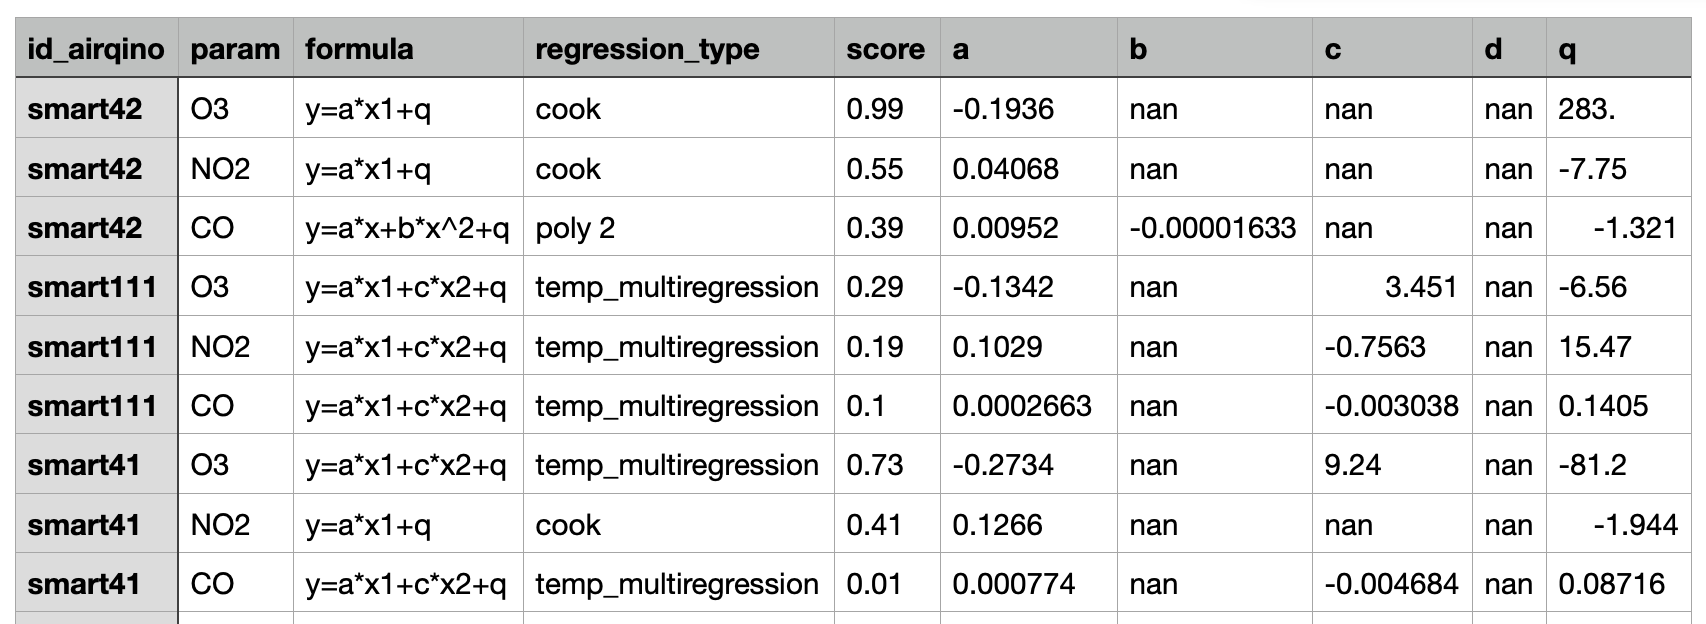
\includegraphics[width=0.75\textwidth,height=\textheight,keepaspectratio]{img/csv_calib}
\caption{Esempio di file csv per calibrazione di centraline AirQino}
\label{fig:csv-calib}
\end{figure}

Dove: 

\begin{itemize}
  \item La colonna \textbf{id\_airqino} indica il nome della centralina AirQino;
  \item La colonna \textbf{param} indica il sensore da calibrare;
  \item Le colonne \textbf{a}, \textbf{b}, \textbf{c} e \textbf{q} rappresentano i coefficienti di calibrazione (rispettivamente \textit{k1}, \textit{k2}, \textit{k3} e \textit{k4} della formula riportata in \ref{sec:motivazioni});
  \item La colonna \textbf{score} indica il coefficiente di determinazione $R^2$;
  \item Le colonne \textbf{formula}, \textbf{regression\_type} e \textbf{d} sono opzionali e riguardano il tipo di regressione e altri parametri al momento inutilizzati (non influiscono sul risultato finale).
\end{itemize}

% Tecnologie utilizzate
\section{Tecnologie utilizzate}\label{sec:tecnologie}

\subsection{Backend}\label{ssec:interfaccia-backend}

\begin{itemize}
  \item \textbf{Flask} \cite{flask} è un framework scritto in Python per la realizzazione di applicazioni web. Ha la caratteristica di essere molto semplice e versatile nella gestione del routing e la creazione di API REST;
  \item \textbf{Pandas} \cite{pandas} è una libreria Python che fornisce strumenti di analisi e manipolazione dei dati. Utilizzata nel progetto per leggere i dati da un file csv;
  \item \textbf{Psycopg2} \cite{psycopg2} è una libreria Python per la connessione a database che utilizzano Postgres (come quello di AirQino);
  \item \textbf{Docker} \cite{docker} è una tecnologia di containerizzazione che consente di organizzare le applicazioni in \textit{container}, componenti isolati che combinano il codice sorgente dell'applicazione con le librerie del sistema operativo e le dipendenze necessarie per eseguire il codice in qualsiasi ambiente. 
\end{itemize}

\clearpage

\subsection{Frontend}\label{ssec:interfaccia-frontend}

\begin{itemize}
  \item \textbf{Angular} \cite{angular} è un framework di applicazioni web, basato su linguaggio TypeScript, che consente la creazione di Single Page Application (SPA) reattive;
  \item \textbf{Bootstrap} \cite{bootstrap} è un framework CSS dedicato allo sviluppo frontend, mettendo a disposizione tipografia, pulsanti, navigazione e altri componenti dell'interfaccia web;
  \item \textbf{ng-bootstrap} \cite{ng-bootstrap} è un set di widget e componenti Angular reattivi che utilizzano lo stile Bootstrap.
\end{itemize}

% Sviluppo
\section{Sviluppo}\label{sec:sviluppo}
Il risultato finale è stato reso disponibile al seguente indirizzo:\

\url{https://airqino-calibration.magentalab.it}.

Di seguito ne vengono descritte le caratteristiche principali.

% Interfaccia
\subsection{Interfaccia}\label{sec:interfaccia}

L'interfaccia, dopo il primo caricamento, si presenta come in figura \ref{fig:interfaccia-1}, con un \textit{form} che permette di scegliere e caricare il file csv, una \textit{checkbox} che consente di aprire una nuova sessione per tutte le centraline, e un pulsante per avviare il caricamento.
\begin{figure}[H]
\centering
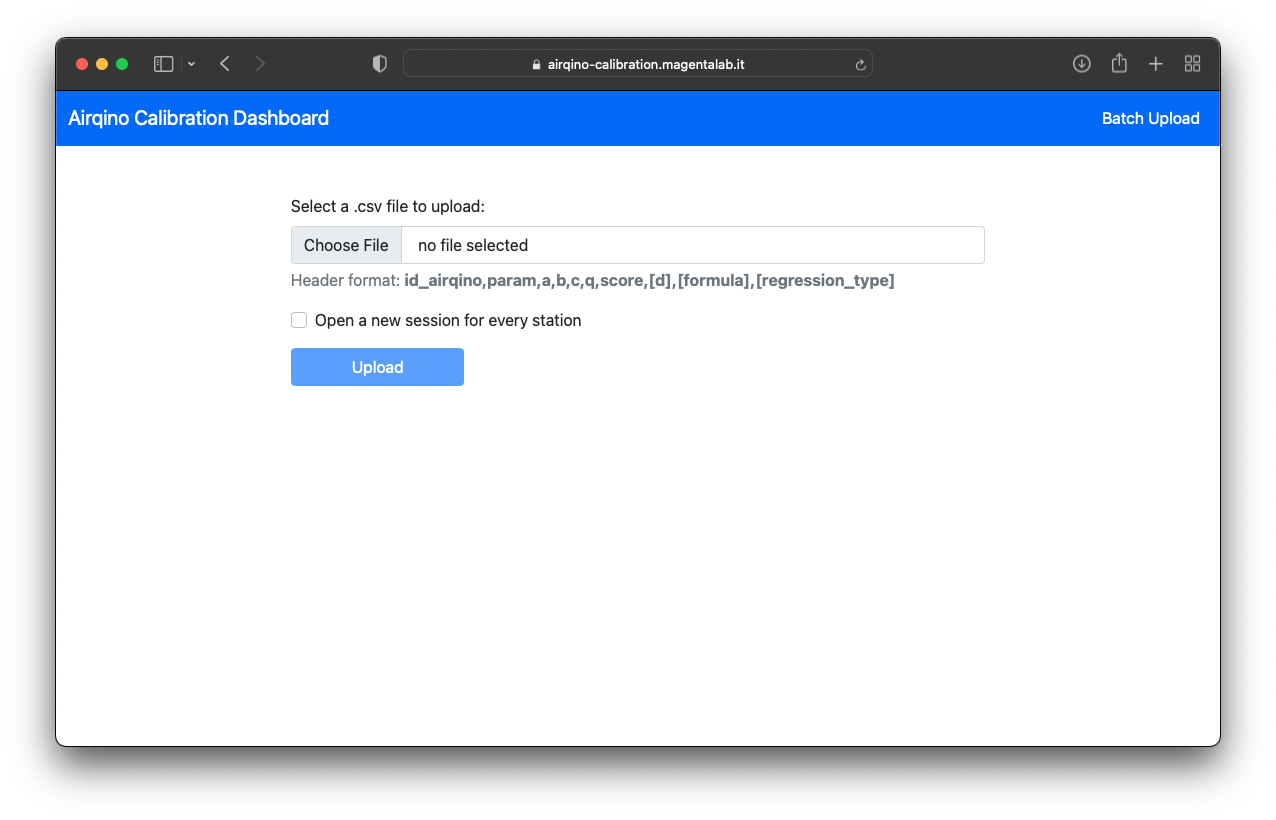
\includegraphics[width=0.70\textwidth,height=\textheight,keepaspectratio]{img/interfaccia_1}
\caption{Interfaccia iniziale dell'applicazione}
\label{fig:interfaccia-1}
\end{figure} 

Se il formato del file csv scelto non è compatibile con quello previsto (vedi \ref{sec:requisiti}), la pagina restituisce un errore informativo dove viene indicata esattamente quali colonne mancano nell'\textit{header} (figura \ref{fig:interfaccia-8}).

\begin{figure}[H]
\centering
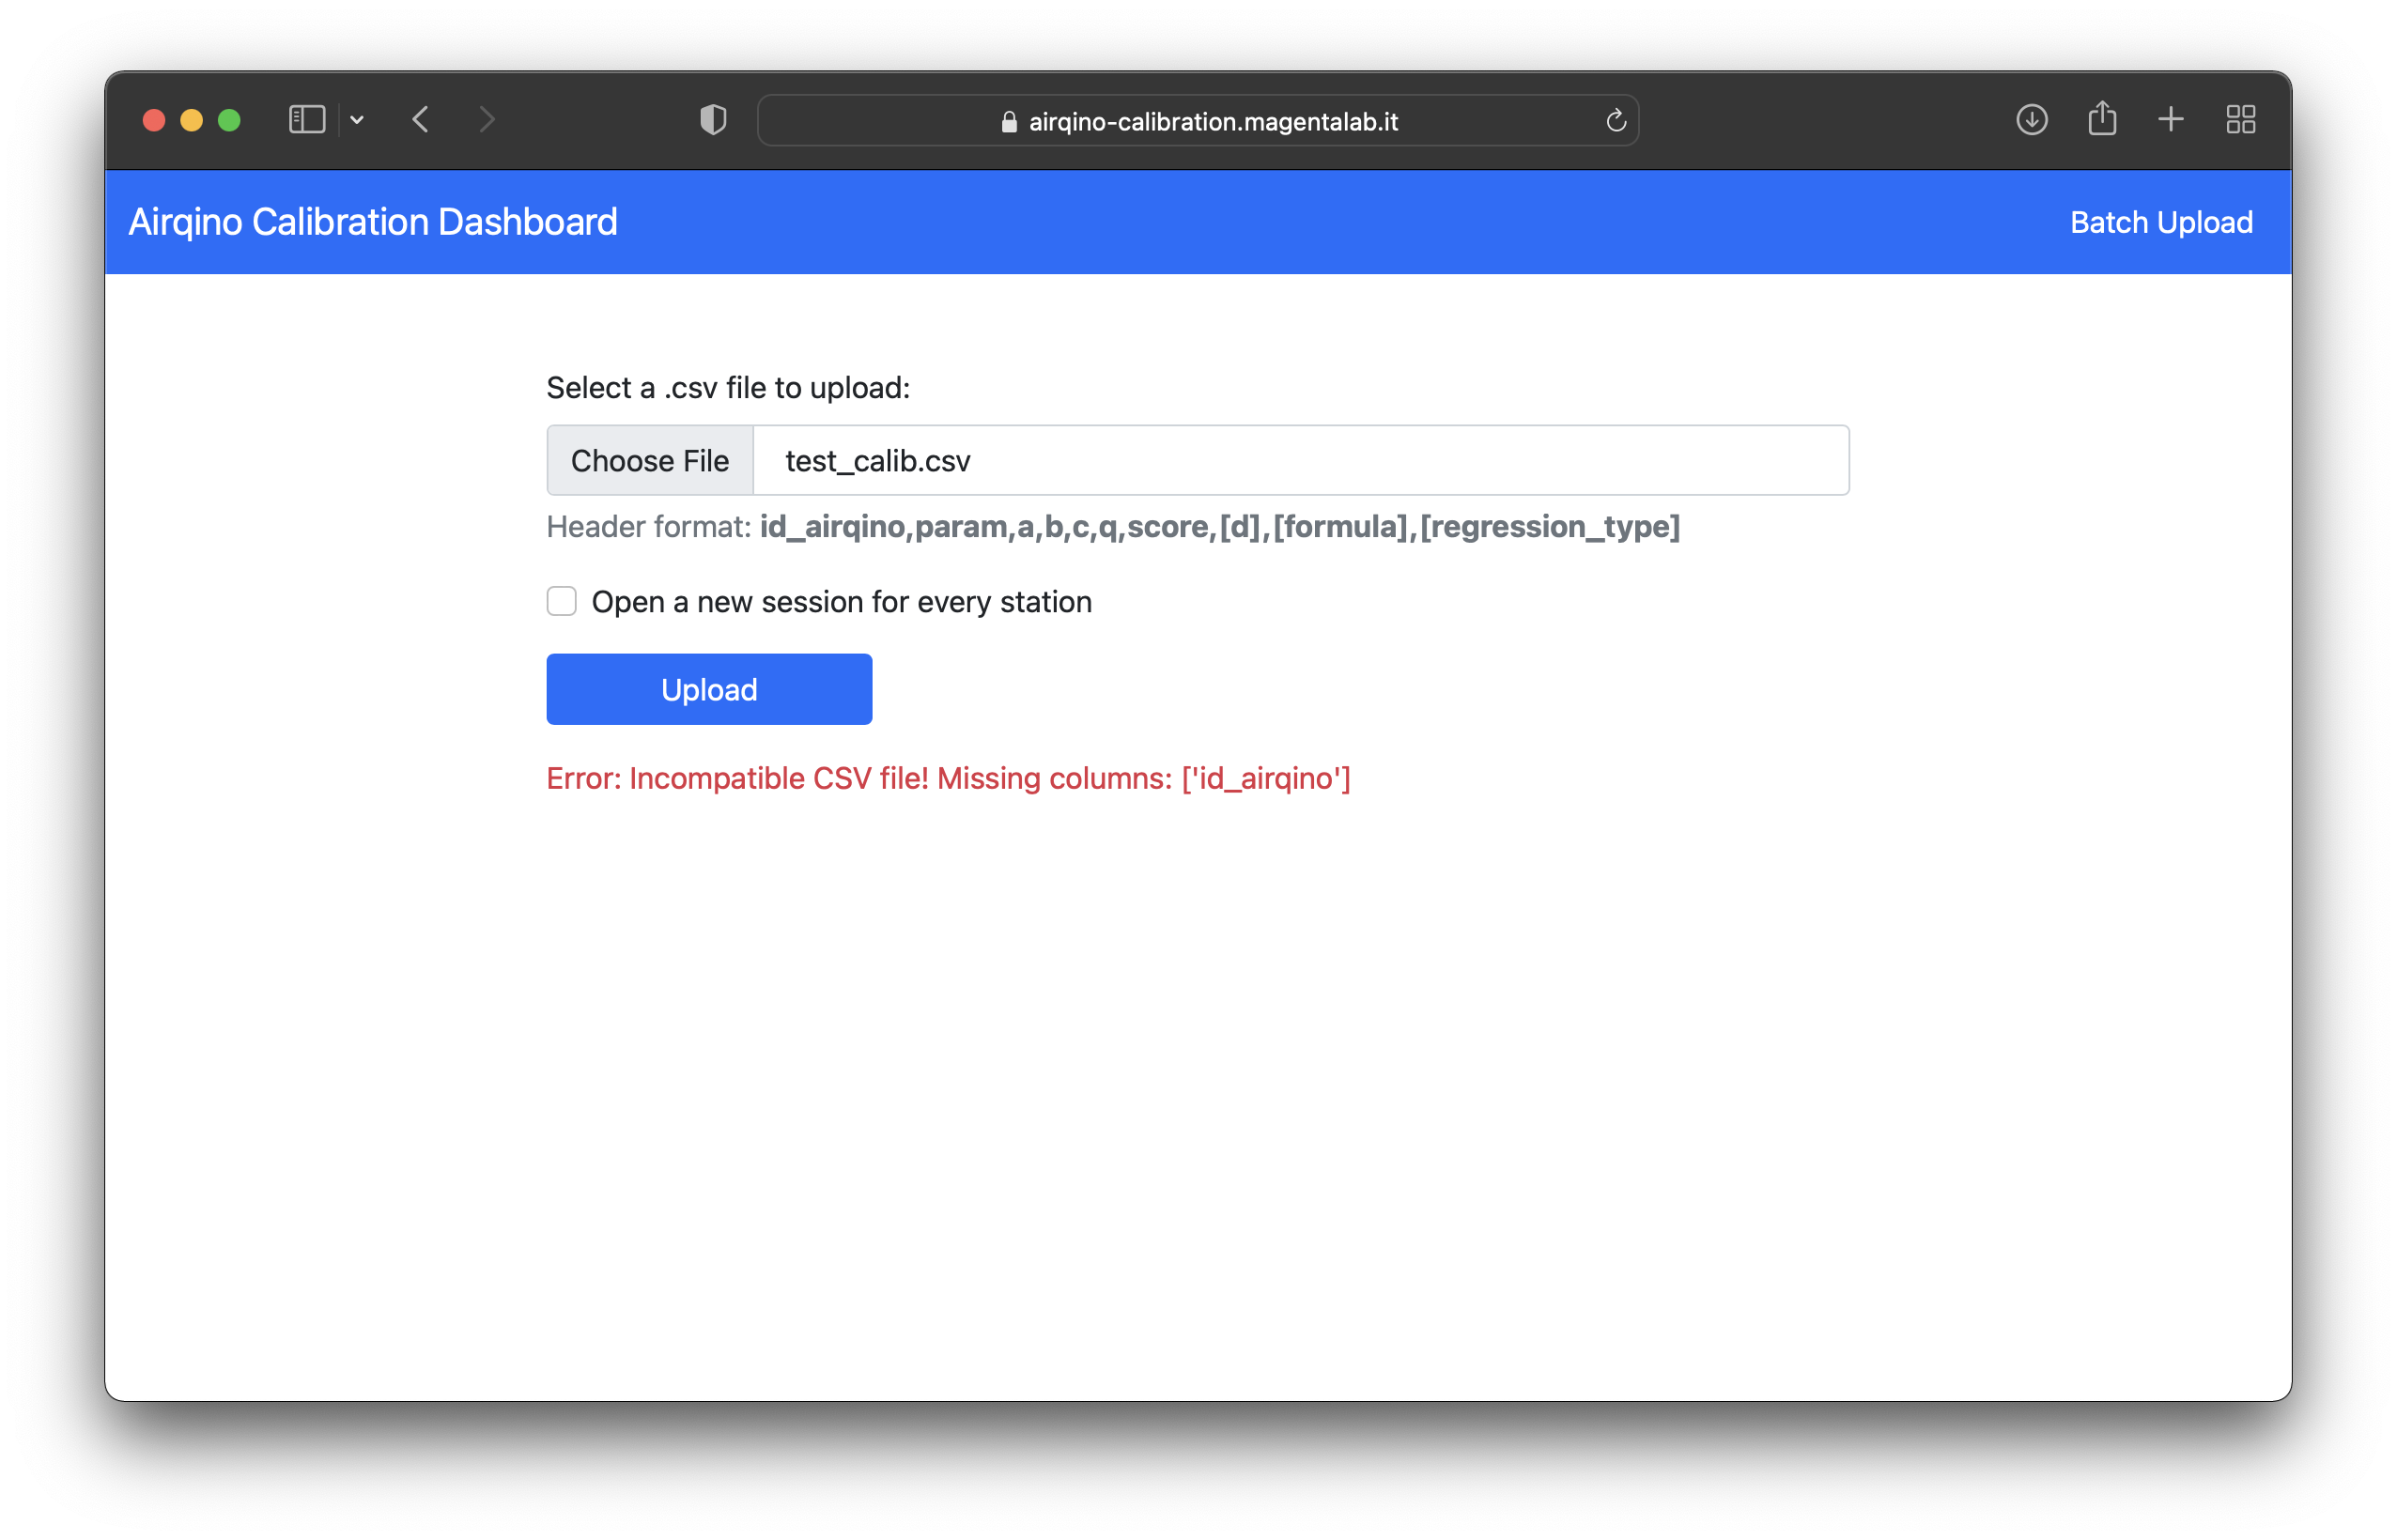
\includegraphics[width=0.70\textwidth,height=\textheight,keepaspectratio]{img/interfaccia_8}
\caption{Errore informativo mostrato in caso di caricamento di un file csv con header non riconosciuto}
\label{fig:interfaccia-8}
\end{figure}

Una pagina simile viene mostrata nel caso in cui l'applicazione non riesca a connettersi al database di AirQino (ad esempio se questo è in fase di mantenimento).

Se il file csv caricato ha il formato corretto, e il database è raggiungibile, viene avviata la procedura di caricamento multiplo dei coefficienti. Al termine dell'operazione, viene mostrato un riepilogo in forma di tabella dove ogni riga corrisponde ad un sensore (figura \ref{fig:interfaccia-2}).

\begin{figure}[H]
\centering
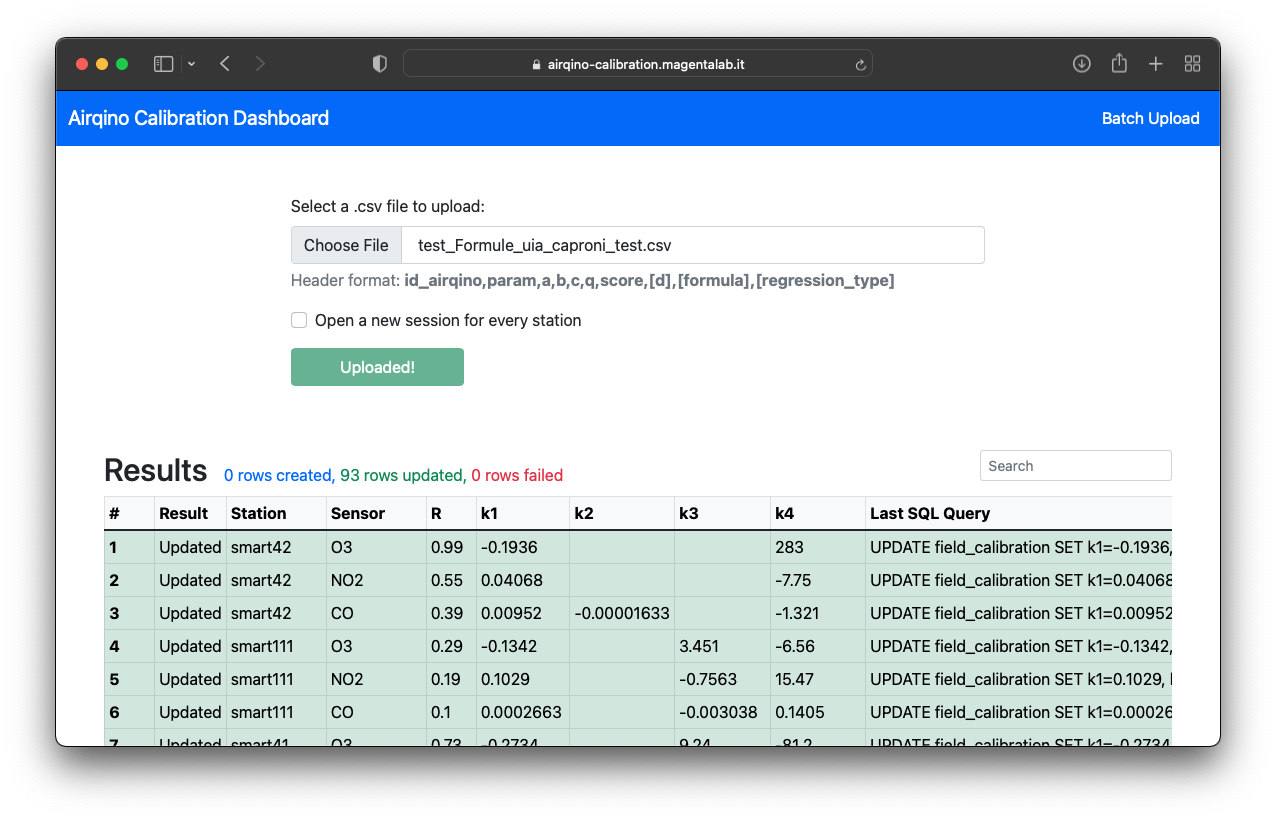
\includegraphics[width=0.70\textwidth,height=\textheight,keepaspectratio]{img/interfaccia_2}
\caption{Interfaccia in caso di caricamento corretto del file csv}
\label{fig:interfaccia-2}
\end{figure}

La tabella, mostrata nel dettaglio in figura \ref{fig:interfaccia-3}, presenta le seguenti colonne:
\begin{itemize}
  \item \textbf{Result}: è l'esito del caricamento sul database (\textit{Updated} se il dato era già presente ed è stato sovrascritto, \textit{Created} se il dato è stato creato per la prima volta, e \textit{Failed} se l'operazione invece è fallita per quel sensore);
  \item \textbf{Station}, \textbf{Sensor}, \textbf{R}, \textbf{k1}, \textbf{k2}, \textbf{k3}, \textbf{k4} sono gli stessi parametri passati nel file csv di input;
  \item \textbf{Last SQL Query}: è l'ultima query effettuata sul database per quel sensore, utile in per verificarne la correttezza e/o capire il motivo di eventuali errori (lo screenshot completo è riportato in figura \ref{fig:interfaccia-6}).
\end{itemize}

\begin{figure}[H]
\centering
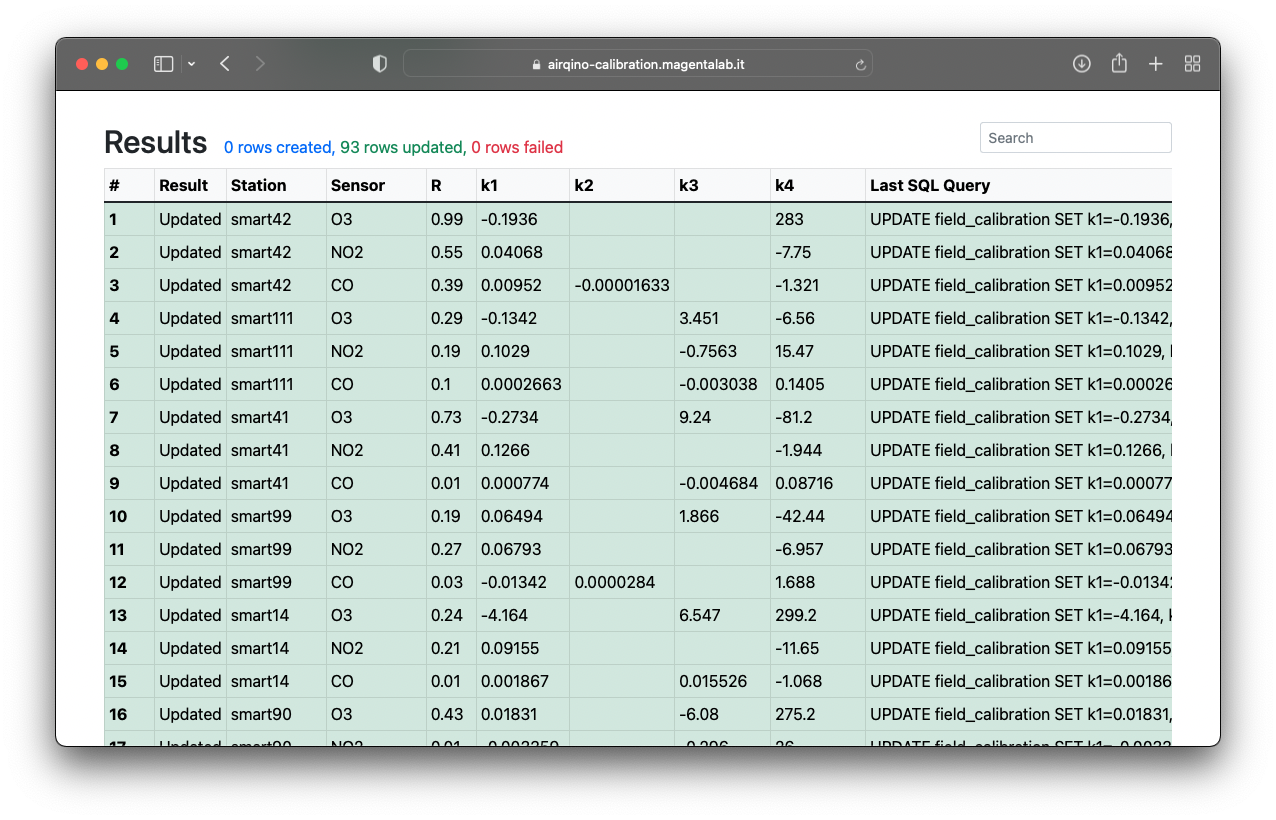
\includegraphics[width=0.70\textwidth,height=\textheight,keepaspectratio]{img/interfaccia_3}
\caption{Dettaglio della tabella di riepilogo del caricamento dei coefficienti}
\label{fig:interfaccia-3}
\end{figure}

\begin{figure}[H]
\centering
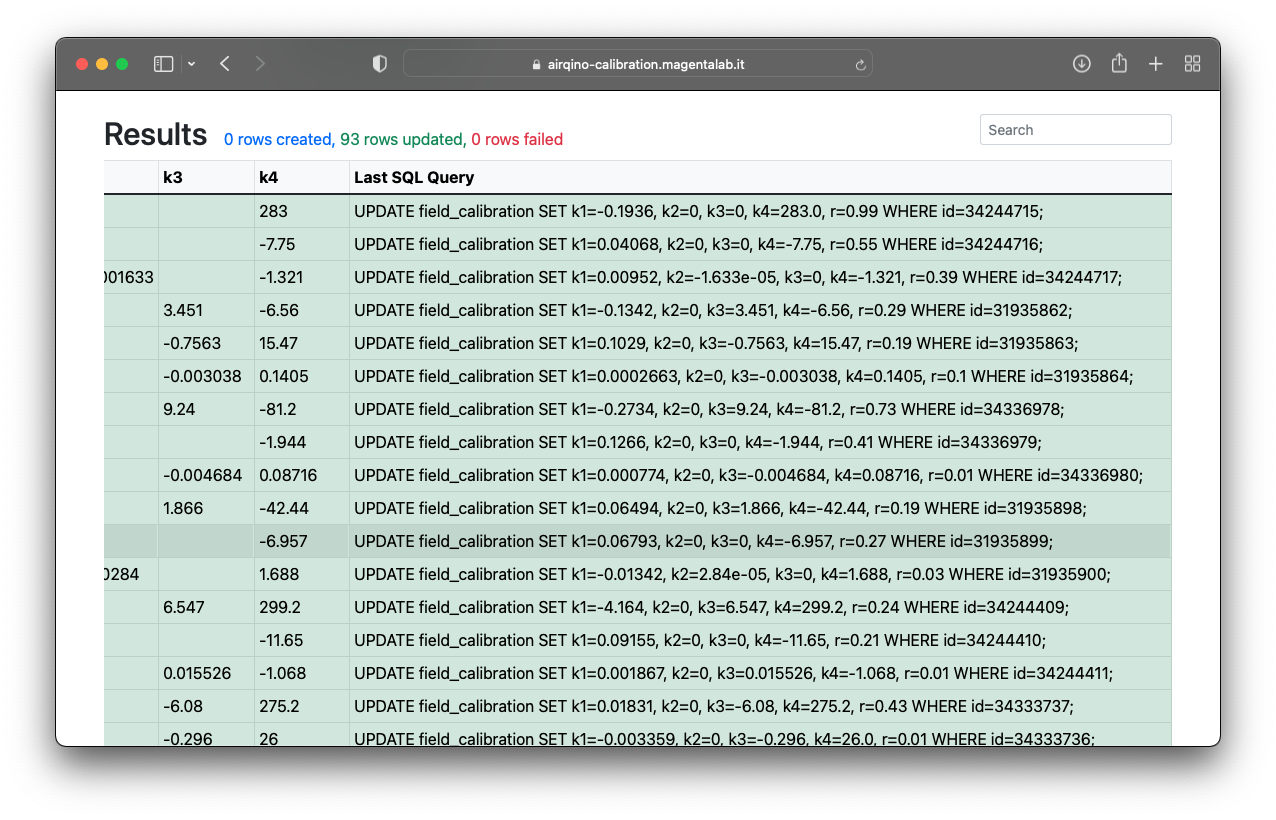
\includegraphics[width=0.70\textwidth,height=\textheight,keepaspectratio]{img/interfaccia_6}
\caption{Dettaglio completo per la colonna \textit{Last SQL Query} della tabella riassuntiva di caricamento dei coefficienti}
\label{fig:interfaccia-6}
\end{figure}

La tabella è ordinabile per colonne (tramite un click su ciascuna di esse) e filtrabile con ricerca \textit{full text} su qualsiasi campo (figura \ref{fig:interfaccia-4-5}).

\begin{figure}[H]%
    \centering
    \captionsetup{justification=centering}
    \subfloat[\centering Ordinamento per colonne]{{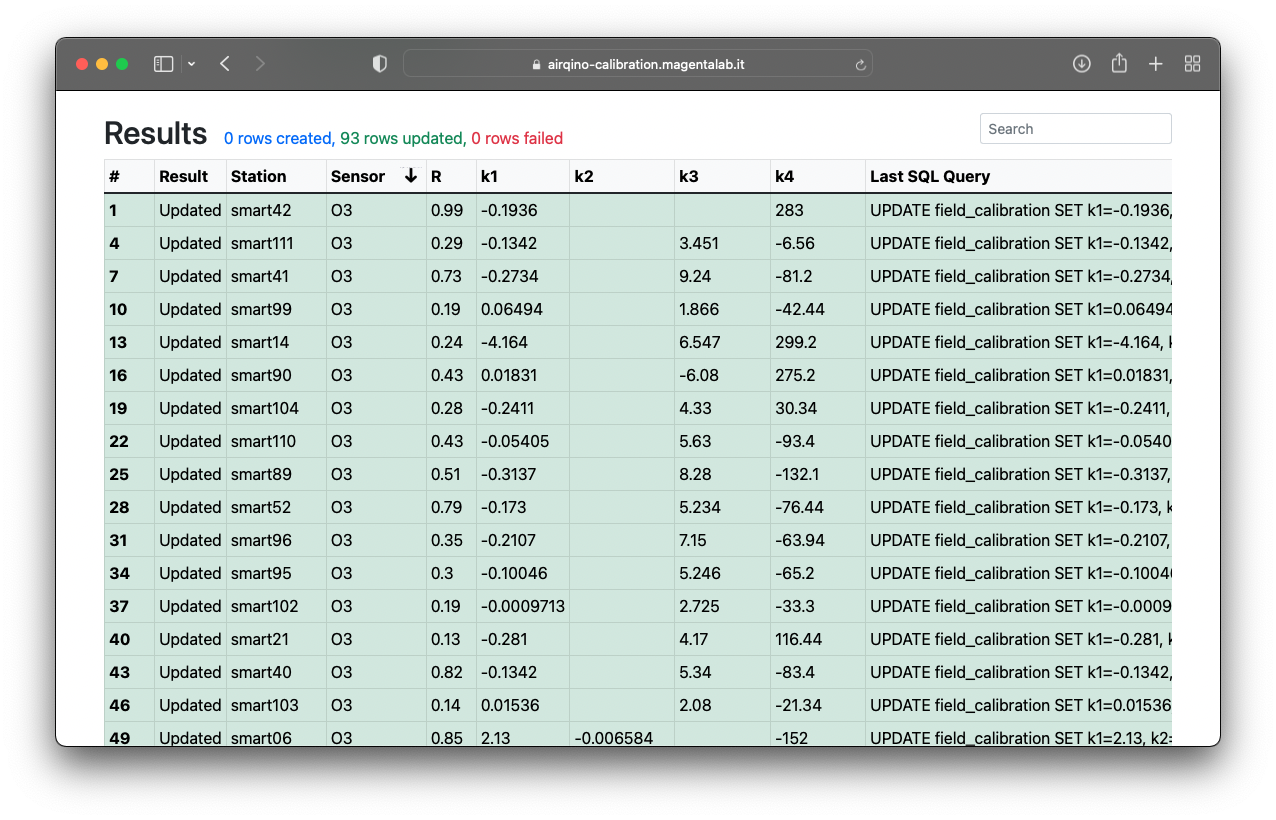
\includegraphics[width=6.9cm]{img/interfaccia_5} }}%
    \subfloat[\centering Filtro con ricerca \textit{full text}]{{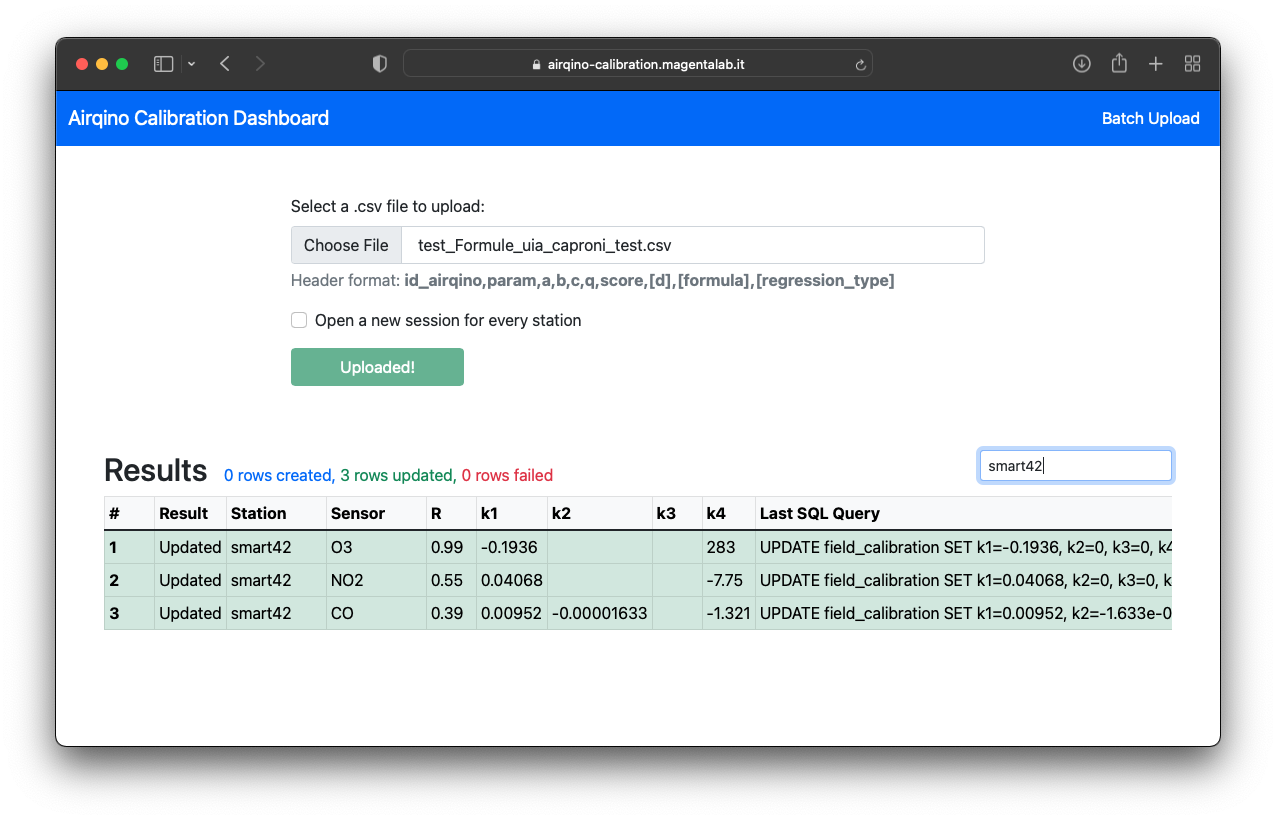
\includegraphics[width=6.9cm]{img/interfaccia_4} }}%
    \caption{Esempio di ordinamento e ricerca della tabella riassuntiva di caricamento dei coefficienti}%
    \label{fig:interfaccia-4-5}%
\end{figure}

In caso di esito negativo per un sensore (ad esempio se il sensore o la centralina specificati non esistono nel database), la riga corrispondente risulta colorata di rosso e la colonna \textbf{Result} fornisce un aiuto nel capire il motivo (es. "Failed: station SMART999 does not exist").
Se invece i coefficienti non erano presenti nel database e sono stati caricati per la prima volta, la riga risulta colorata di azzurro. La figura \ref{fig:interfaccia-7} riporta un esempio di diversa colorazione delle righe in base all'esito: verde per coefficienti aggiornati, rosso per caricamento fallito e azzurro per coefficienti aggiunti per la prima volta.

\vspace{2mm}
\begin{figure}[H]
\centering
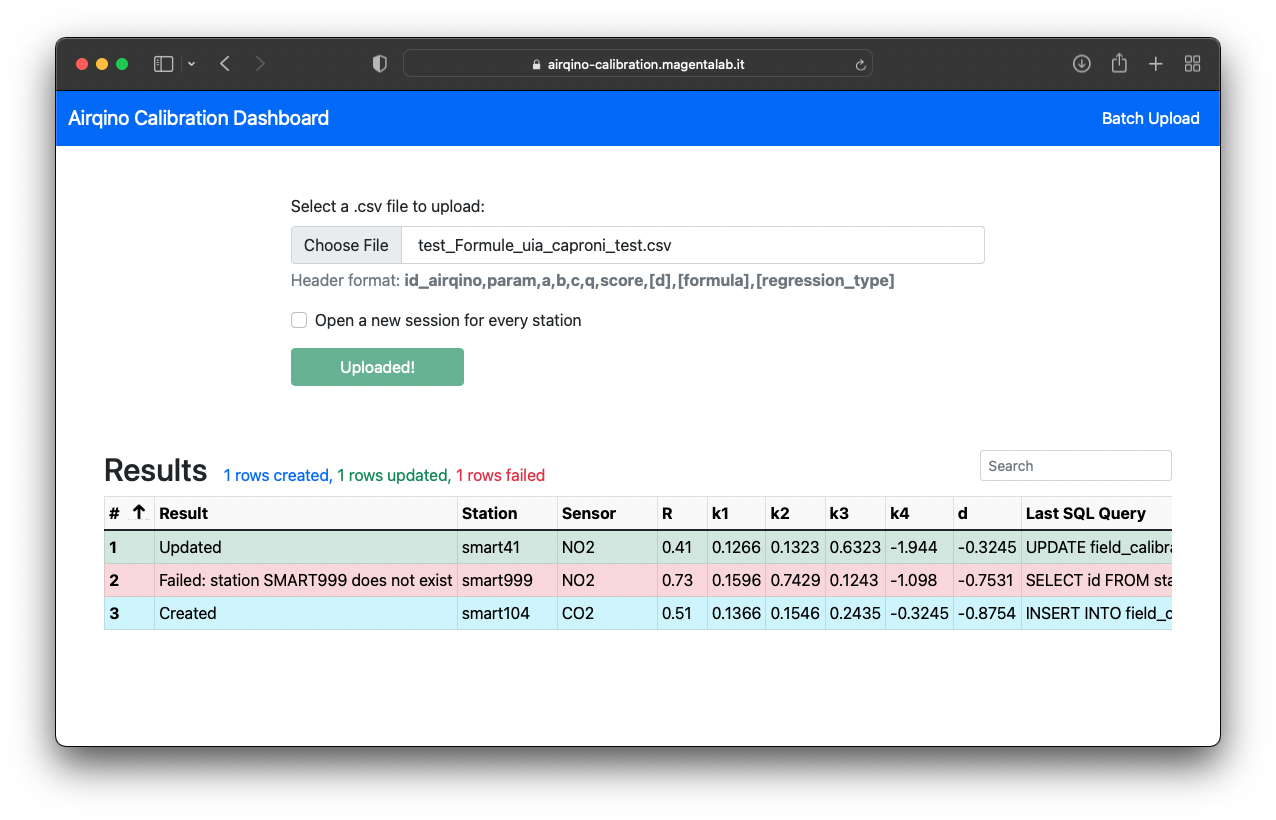
\includegraphics[width=0.60\textwidth,height=\textheight,keepaspectratio]{img/interfaccia_7}
\caption{Esempio di colorazione delle righe della tabella}
\label{fig:interfaccia-7}
\end{figure}

% Autenticazione
\subsection{Autenticazione}\label{sec:autenticazione}
Per la gestione dell'autenticazione è stato scelto il software \textbf{Keycloak} \cite{keycloak}, che risultava essere già installato sul server di Magenta. Keycloak è un prodotto software open source che abilita l'autenticazione \textit{Single Sign-On} (SSO) per applicazioni e servizi. È scritto in Java e supporta i protocolli di federazione delle identità per impostazione predefinita SAML v2 e OpenID Connect (OIDC) o OAuth2. \cite{keycloak_art}

In particolare, Keycloak consente a un'applicazione di delegare la propria autenticazione ad un server web predisposto, consentendo allo sviluppatore di concentrarsi sulle funzionalità, senza doversi preoccupare di aspetti di sicurezza e crittografia. Keycloak infatti include un server e un agente: l'agente è installato sulle applicazioni che richiedono l'autenticazione, mentre il server gestisce tutte le richieste di autenticazione. Quando un utente tenta di accedere a una applicazione protetta da Keycloak, l'agente verifica se l'utente è autenticato e, in caso affermativo, fornisce le credenziali appropriate all'applicazione.

\begin{figure}[H]
\centering
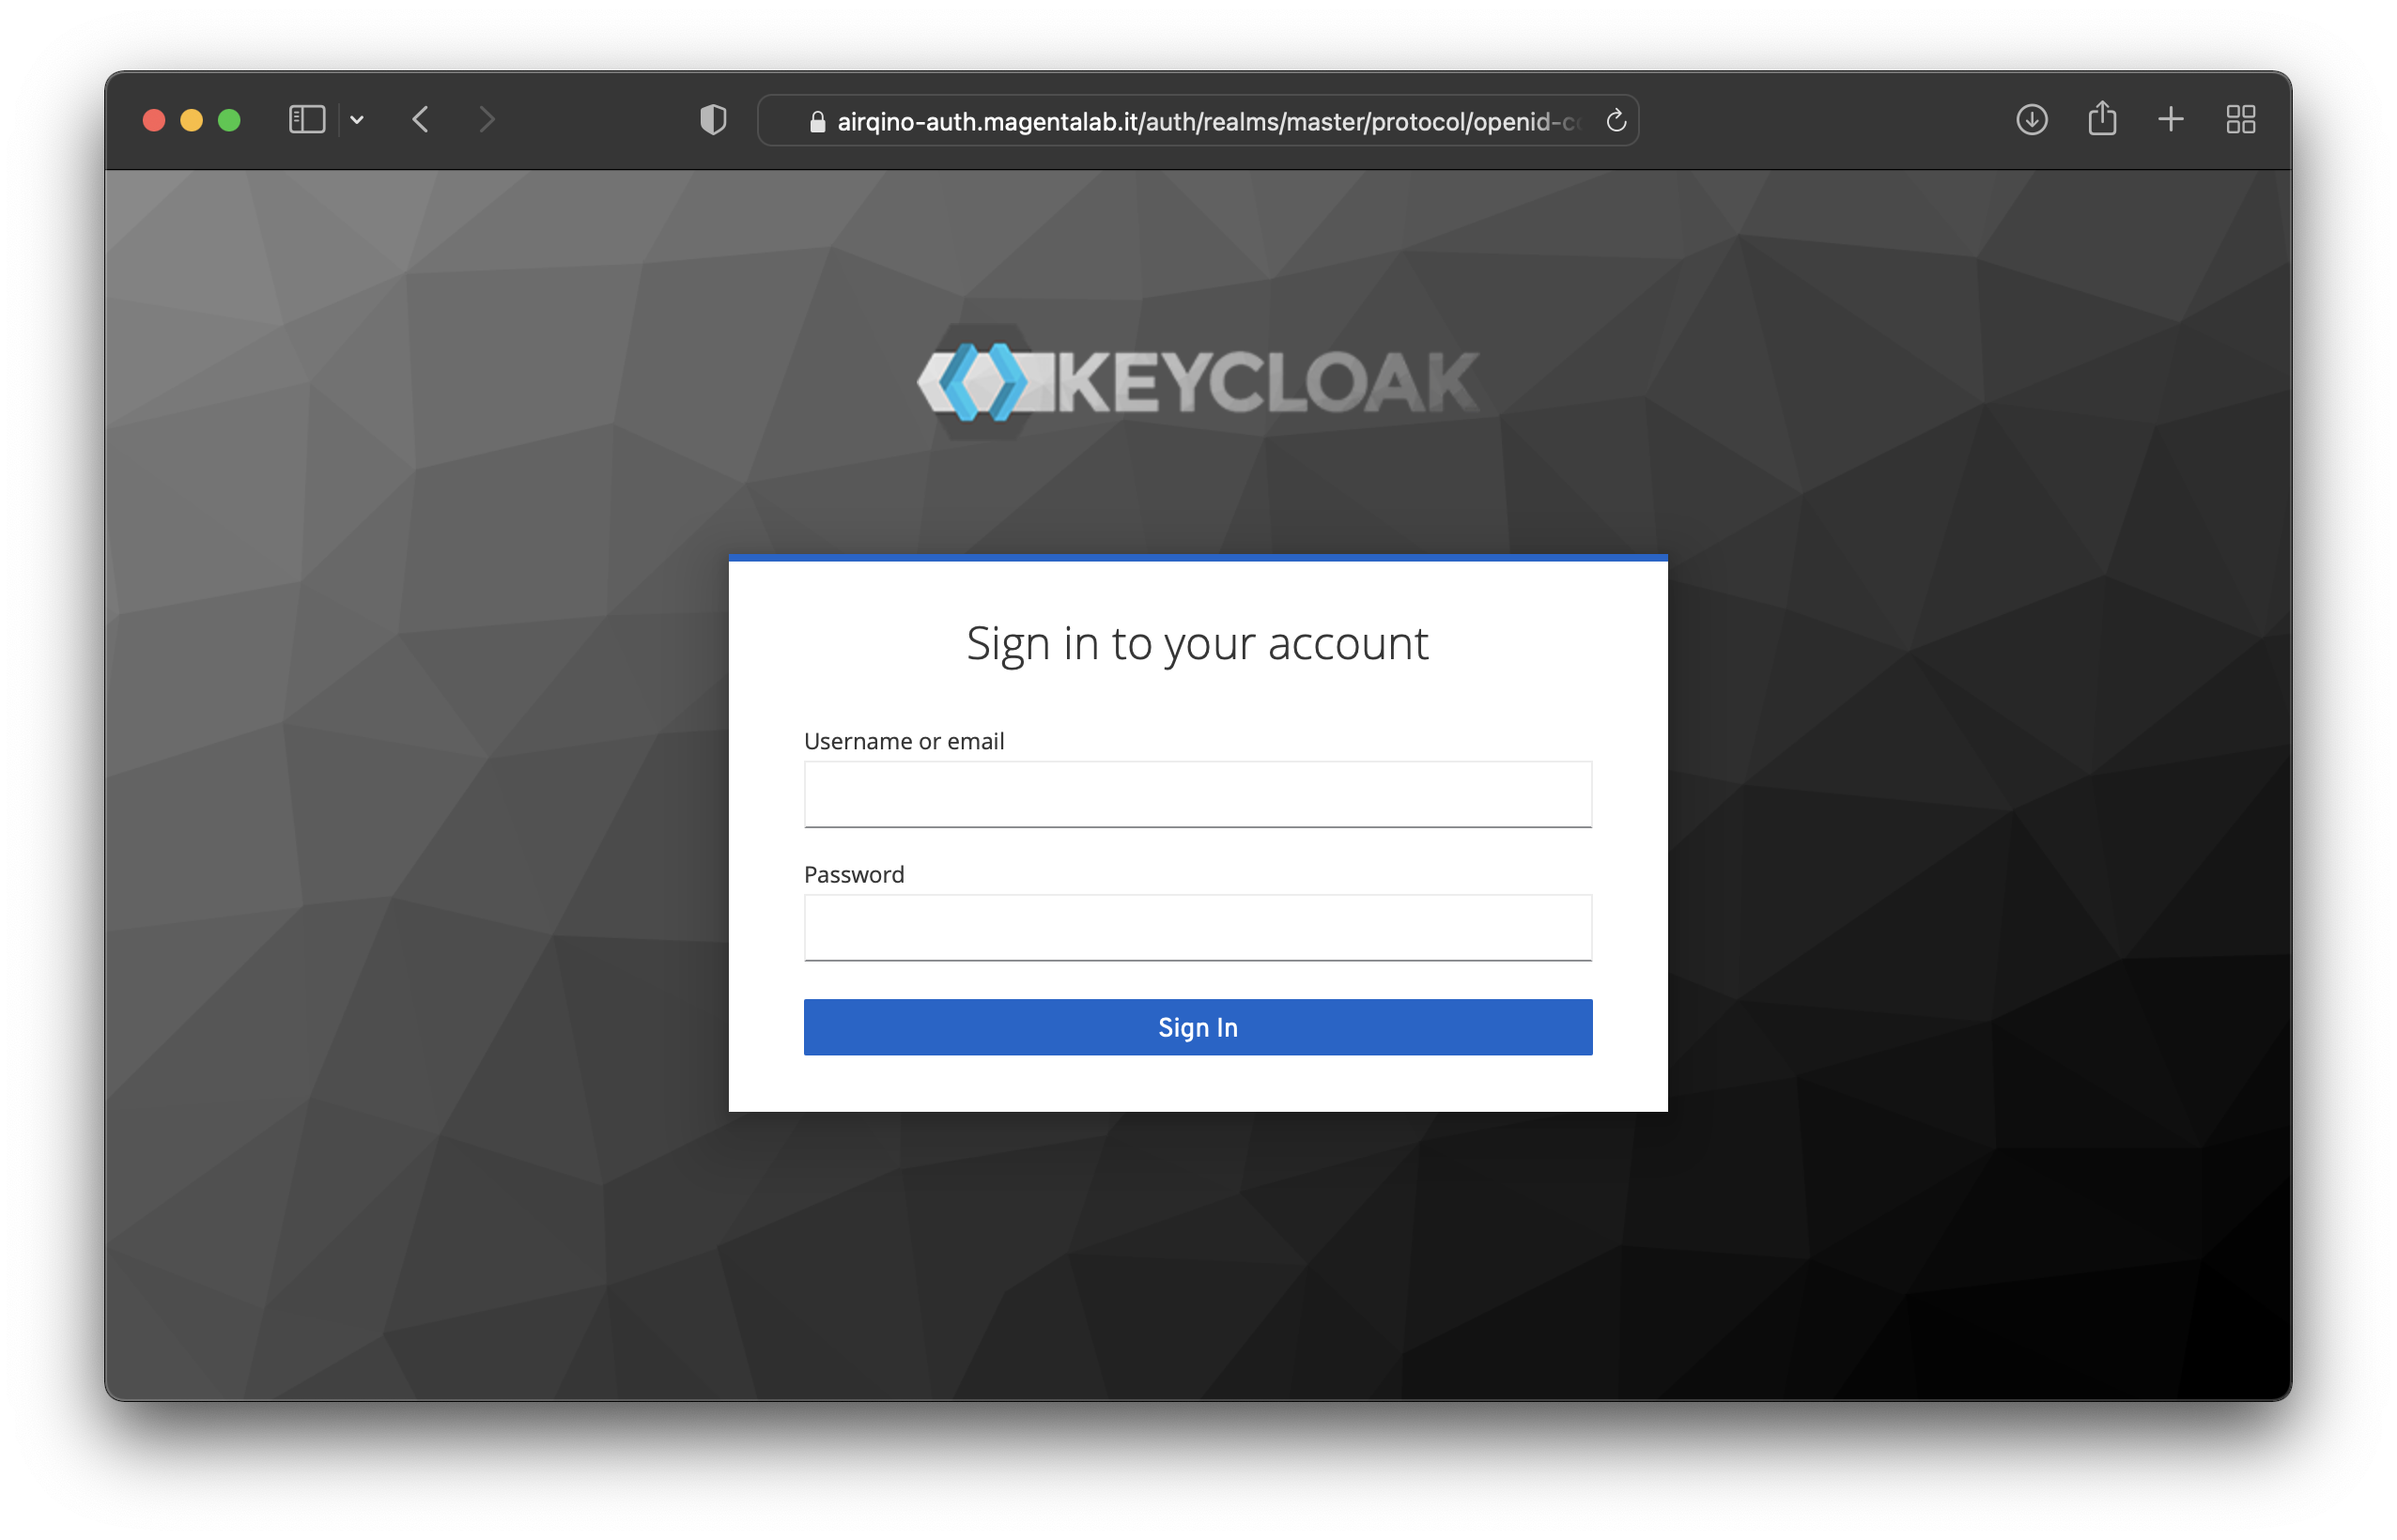
\includegraphics[width=0.70\textwidth,height=\textheight,keepaspectratio]{img/keycloak}
\caption{Autenticazione con Keycloak}
\label{fig:keycloak}
\end{figure}

Keycloak è stato integrato nell'applicazione con l'aiuto della libreria open source \url{keycloak-angular} \cite{keycloak-angular}, un wrapper della libreria ufficiale JavaScript \url{keycloak-js} \cite{keycloak-js} che rende semplice l'utilizzo del software per applicazioni Angular. I principali parametri da impostare sono:

\begin{itemize}
  \item \textbf{url}: l'url del server Keycloak;
  \item \textbf{realm}: il nome del \textit{realm}, impostato nel pannello di amministrazione, che serve a gestire un insieme di utenti, credenziali e ruoli;
  \item \textbf{clientId}: l'identificativo del \textit{client}, cioè l'entità che richiede a Keycloak il permesso di autenticare un utente, anche questo impostato nel pannello di amministrazione;
  \item \textbf{initOptions}: le opzioni di configurazione, ad esempio è possibile specificare se l'autenticazione avviene automaticamente al caricamento della pagina (come in questo caso) oppure scatta in un secondo momento (utile se ad esempio l'applicazione fornisce funzionalità anche senza loggare l'utente).
\end{itemize}

È possibile inizializzare la configurazione in un file JavaScript di questo tipo (file \url{keycloak-init.js}, da caricare poi all'avvio del modulo principale dell'applicazione):

\vspace{1mm}
\begin{lstlisting}[language=js]
import {KeycloakService} from "keycloak-angular";

export function initializeKeycloak(keycloak: KeycloakService) {
  return () =>
    keycloak.init({
      config: {
        url: 'https://airqino-auth.magentalab.it/auth',
        realm: 'master',
        clientId: 'calibration',
      },
      initOptions: {
        onLoad: 'login-required',
        flow: 'implicit'
      },
    });
}
\end{lstlisting}

Questi parametri sono sufficienti a definire l'integrazione tra applicazione e server Keycloak, garantendo in maniera efficiente funzionalità di autenticazione e autorizzazione.

% CI/CD e deploy automatico
\subsection{CI/CD e deploy automatico}\label{sec:ci}
L'integrazione continua (\textit{continuous integration}, CI o CI/CD) è una metodologia di sviluppo software \textit{agile}, spesso utilizzata in combinazione con approccio \textbf{DevOps}, che prevede la continua e costante integrazione dei cambiamenti effettuati dagli sviluppatori all'interno di un codice sorgente (figura \ref{fig:cicd}).

Con il termine CD (\textit{continuous delivery}) si indica invece la distribuzione e/o il deployment continuo, un concetto comunque correlato alla CI, ovvero processo con il quale le modifiche apportate da uno sviluppatore all'applicazione vengono automaticamente testate e caricate in una repository, dalla quale vengono automaticamente distribuite in un ambiente di produzione. \cite{cicd}

\begin{figure}[H]
\centering
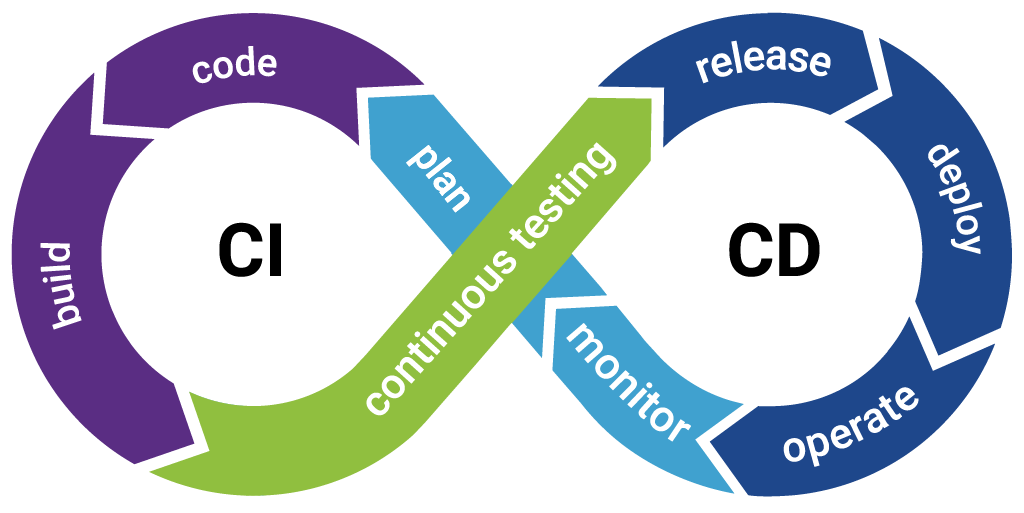
\includegraphics[width=0.65\textwidth,height=\textheight,keepaspectratio]{img/ci}
\caption{Schema di funzionamento CI/CD\\Fonte: \url{flagship.io}}
\label{fig:cicd}
\end{figure}

La CI/CD porta diversi vantaggi, tra cui:
\begin{itemize}
  \item Solidità del prodotto, poiché le integrazioni sono frequenti e anche i test vengono eseguiti in anticipo;
  \item Aumento della qualità del codice;
  \item Consegna più rapida del software.
\end{itemize}

Lo strumento di CI scelto per questa applicazione è \textbf{Jenkins} \cite{jenkins}. Si tratta di un software open source di integrazione continua, scritto in Java, che permette di automatizzare il processo di integrazione dei cambiamenti all'interno di un codice sorgente, con la possibiltà di eseguire una serie di controlli per verificarne la correttezza.\\

Tra le varie caratteristiche, Jenkins offre un sistema chiamato \textit{pipeline}, ovvero uno script (chiamato \textit{Jenkinsfile}) che fornisce a Jenkins una serie di lavori (\textit{stage}) da eseguire in modo simile a una pipeline (uno dopo l'altro).

Il \url{Jenkinsfile} utilizzato per questo progetto contiene tre stage, ognuno con i propri comandi, ed è riportato di seguito (ridotto per semplicità):

\vspace{1mm}
\begin{lstlisting}[]
pipeline {
    agent any
    stages {
		stage('Build Angular frontend') {
			steps {
			    sh 'npm install && ng build --configuration production'
			}
		}
		stage('Docker deploy backend') {
			steps {
				sh 'flask run'
			}
		}
		stage('Deploy frontend') {
			steps {
			    'scp -r dist/* ${HOST}:${PATH}/'
			}
		}
    }
}
\end{lstlisting}

In particolare:

\begin{itemize}
  \item Il primo stage esegue il build del frontend, installando le dipendenze con \url{npm} \url{install} e avviando il processo con \url{ng} \url{build} in configurazione di produzione. Questo genera l'artefatto finale all'interno della cartella \url{dist};
  \item Il secondo stage esegue il rilascio del backend con il comando \url{flask} \url{run};
  \item Infine, il terzo stage rilascia il frontend copiando i contenuti della cartella \url{dist} nella cartella corretta del server di produzione.
\end{itemize}

L'interfaccia web di Jenkins permette inoltre di monitorare l'andamento dei vari step e di verificare eventuali errori. Jenkins può essere anche combinato con Docker \cite{docker} in modo da garantire processi di rilascio automatizzati e allo stesso tempo avere l'isolamento delle dipendenze, che verranno installate solo sul container e non su tutto il server.


\chapter*{Conclusioni e sviluppi futuri}\label{ch:conclusioni}
\addcontentsline{toc}{chapter}{Conclusioni e sviluppi futuri}

\addcontentsline{toc}{chapter}{Bibliografia}
\bibliographystyle{ieeetr}
\bibliography{files/bibliografia}
%\bibliography{sp,xml}

\end{document} 